\documentclass[a4paper, 12pt]{report}

\usepackage{amsmath}
\usepackage{esint}
\usepackage{comment}
\usepackage{amssymb}
\usepackage{commath}
\usepackage{geometry}
\usepackage{graphicx}
\usepackage{hyperref}
\usepackage{listings}
\usepackage{xcolor}
\usepackage{array}

\definecolor{codegreen}{rgb}{0,0.6,0}
\definecolor{codegray}{rgb}{0.5,0.5,0.5}
\definecolor{codepurple}{rgb}{0.58,0,0.82}
\definecolor{backcolour}{rgb}{0.95,0.95,0.92}

\def\t{\theta}
\def\a{\alpha}
\def\be{\beta}
\def\w{\omega}
\def\la{\lambda}
\def\g{\gamma}
\def\f{\frac}
\def\l{\left}
\def\r{\right}
\def\dst{\displaystyle}
\def\b{\bar}
\def\h{\hat}
\def\ph{\phi}
\def\d{\cdot}
\def\n{\nabla}
\def\p{\partial}
\def\lap{\mathcal{L}}
\def\size{0.92}
\def\tabsize{2.7cm}
\def\ltabsize{5.5cm}

%\let\stdsection\section
%\renewcommand\section{\newpage\stdsection}
\geometry{portrait, margin= 0.4in}

\begin{document}

\title{Solution Analysis}
\author{Hans C. Suganda}
\date{$24^{th}$ October 2021}
\maketitle
\newpage

\lstset{
	columns=fullflexible,
	frame=single,
	breaklines=true,
	backgroundcolor=\color{backcolour},   
	commentstyle=\color{codegreen},
	keywordstyle=\color{magenta},
	numberstyle=\tiny\color{codegray},
	stringstyle=\color{codepurple},
	basicstyle=\ttfamily\footnotesize,
	keepspaces=true,                 
	numbersep=5pt,                  
	showspaces=false,               
	showtabs=false,                  
	tabsize=2
}

\tableofcontents
\newpage

\begin{center}
%Seperator
%Seperator
%Seperator
\section{General Training Parameters \& Rationale}
\begin{comment}
\end{comment}
There are infinitely many neural network architecture possibilities. Since the testing choices are somewhat arbitrary, the testing choices for the neural network is systemized by depth of the layers and breadth of the layers. For each test, the neural network is set to have uniform breadth in all of its hidden layers with the same activation functions. It is hoped that the error and solution for somewhat arbitrary neural networks of uniform hidden layer breadth could be somewhat predicted by the results shown here. A single Neural network is used to predict the solution to the Helmholtz equation on a domain $[0,4]$. Since the limits of the neural network architecture is of interest, the neural networks are trained over $50 000$ iterations. This is as large as realistically possible within certain practical limitations and is assumed that the neural network would have converged sufficiently within the training parameter, such that error between the neural network predictions and the analytical solution can be mostly attributed to the neural network architecture and the general ability of said architecture to represent the solution.

%Seperator
%Seperator
%Seperator
\section{Neural Network Depth Study}
\begin{comment}
\end{comment}
The trained neural network's outputs are plotted along with the analytical solution to the problem. In all the plots below, each layer has $100$ nodes and the activation functions are all set to hyperbolic tangent except for the output layer whose activation is set to linear. For hidden layers of depth $4$, the neural network output and analytical solution,
\\~\\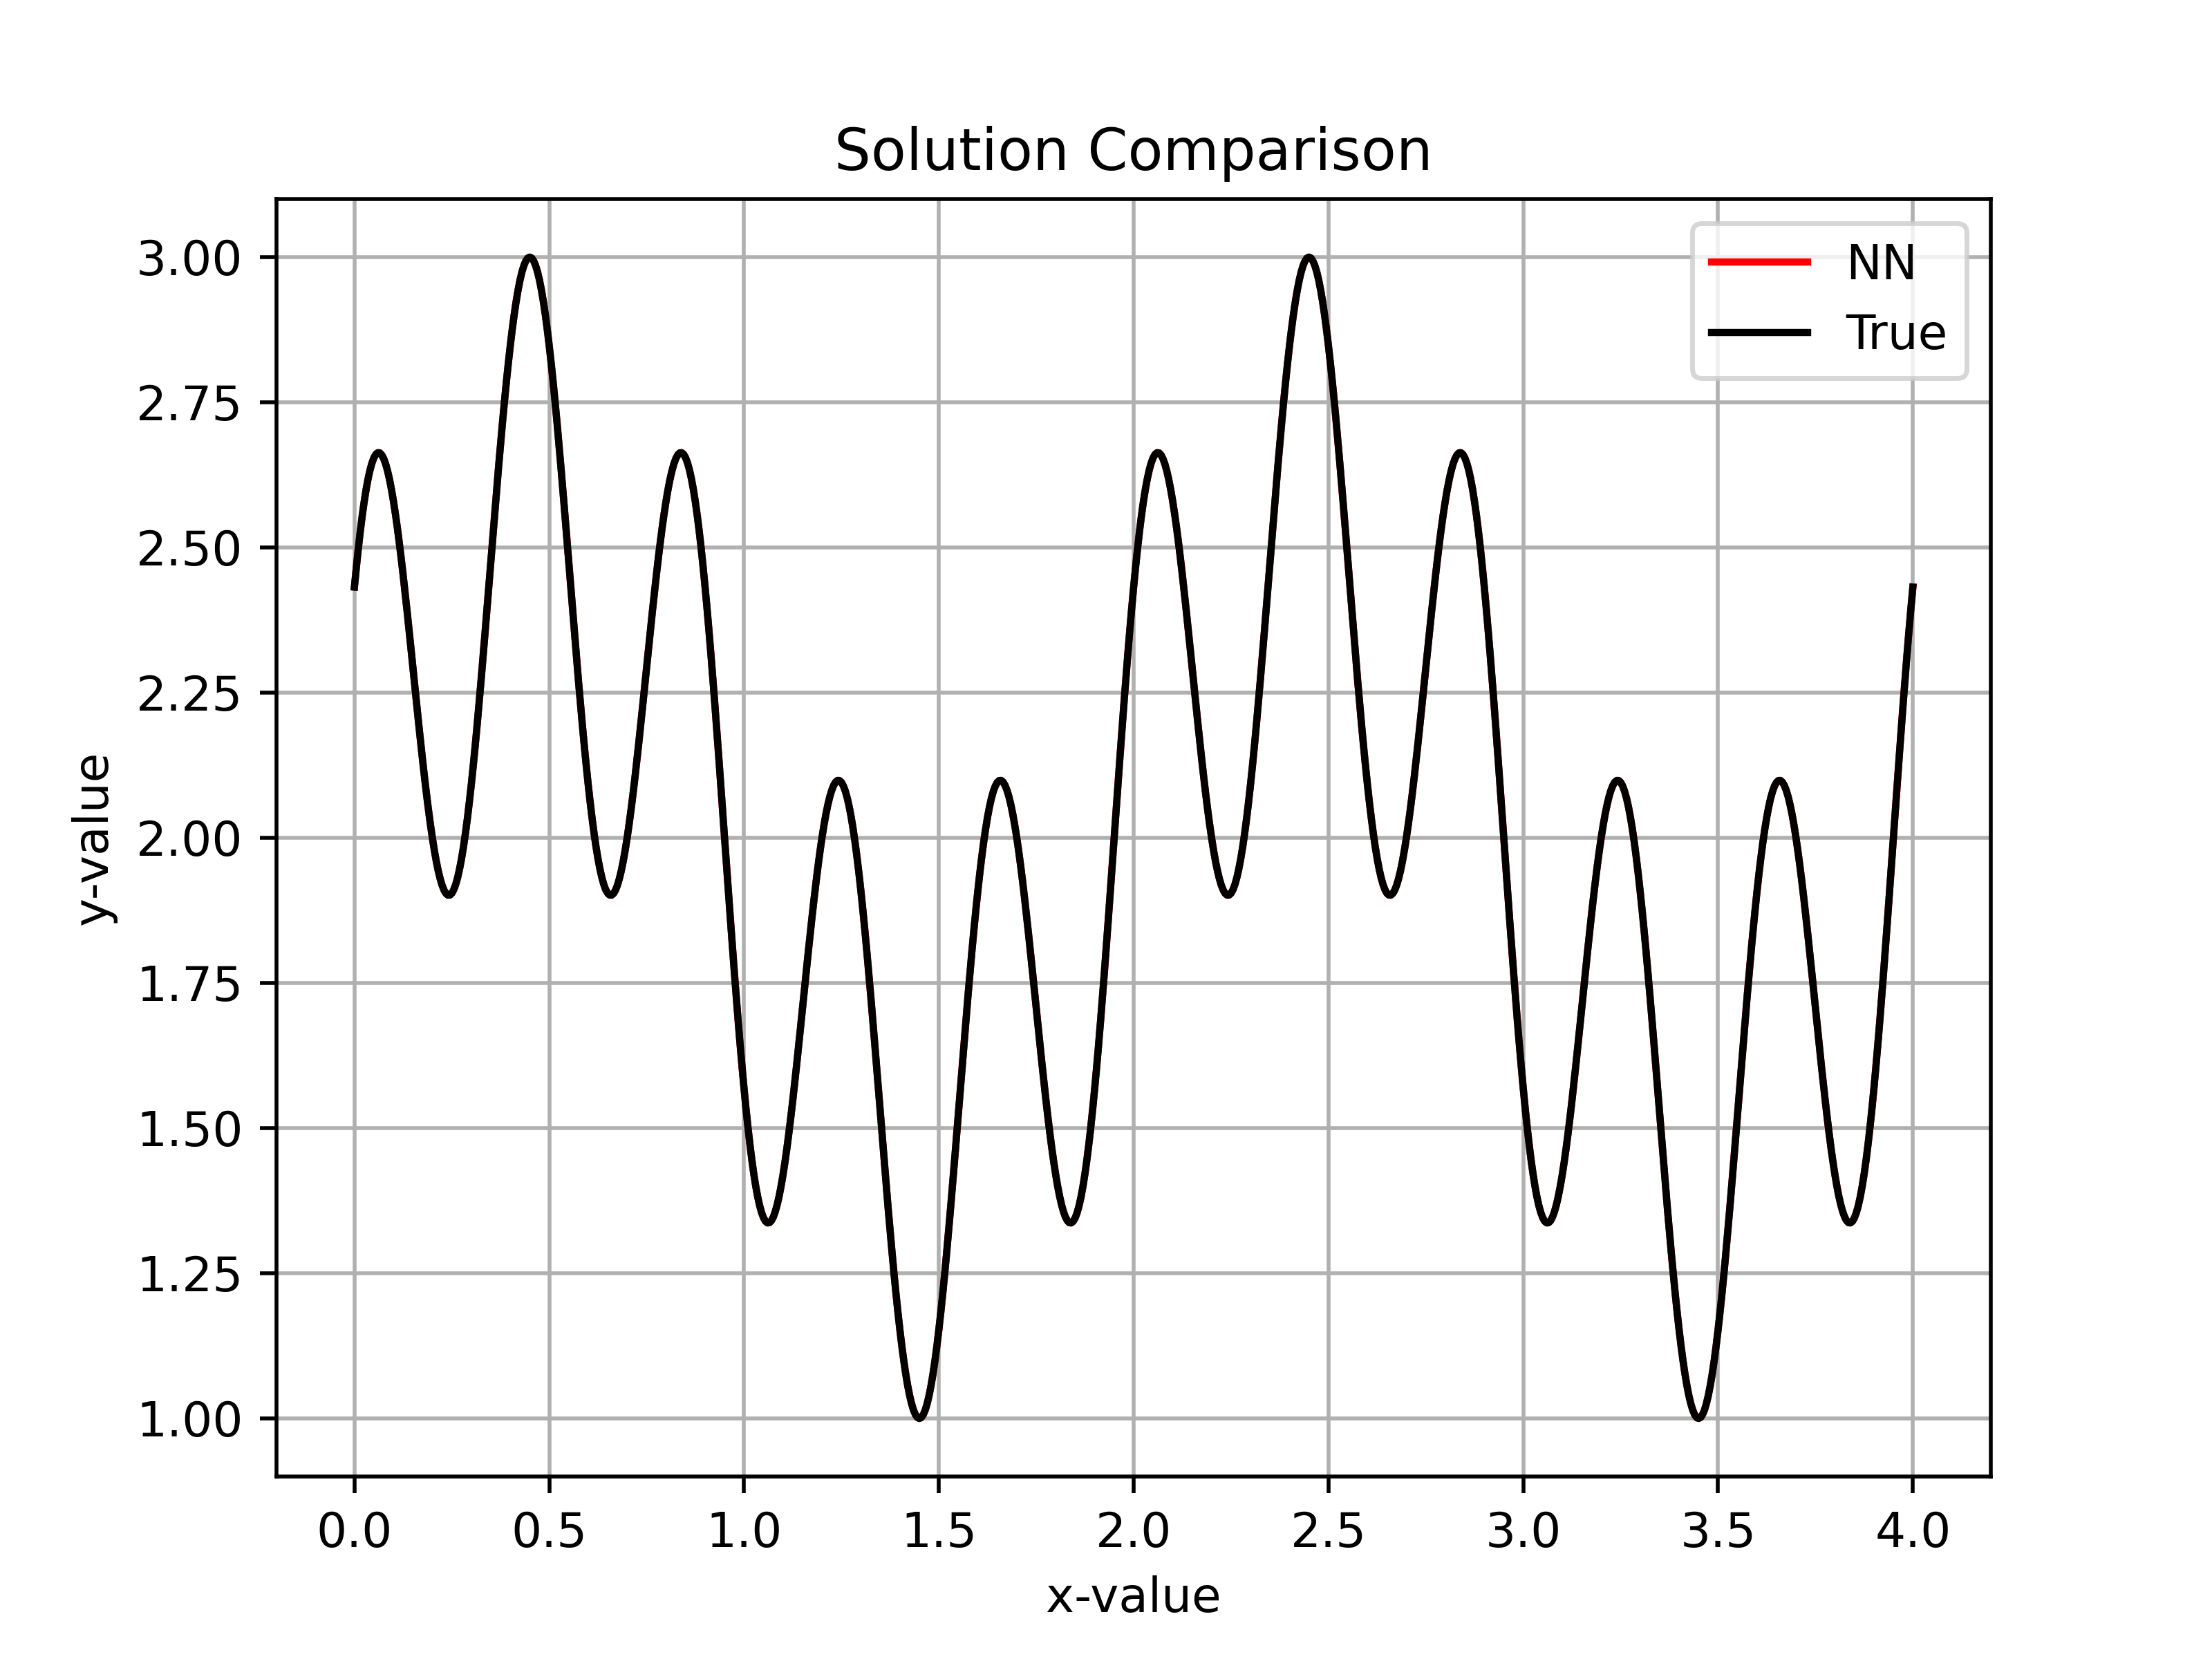
\includegraphics[scale=\size]{depthsol4.png}
\\~\\The corresponding error along the length of the domain,
\\~\\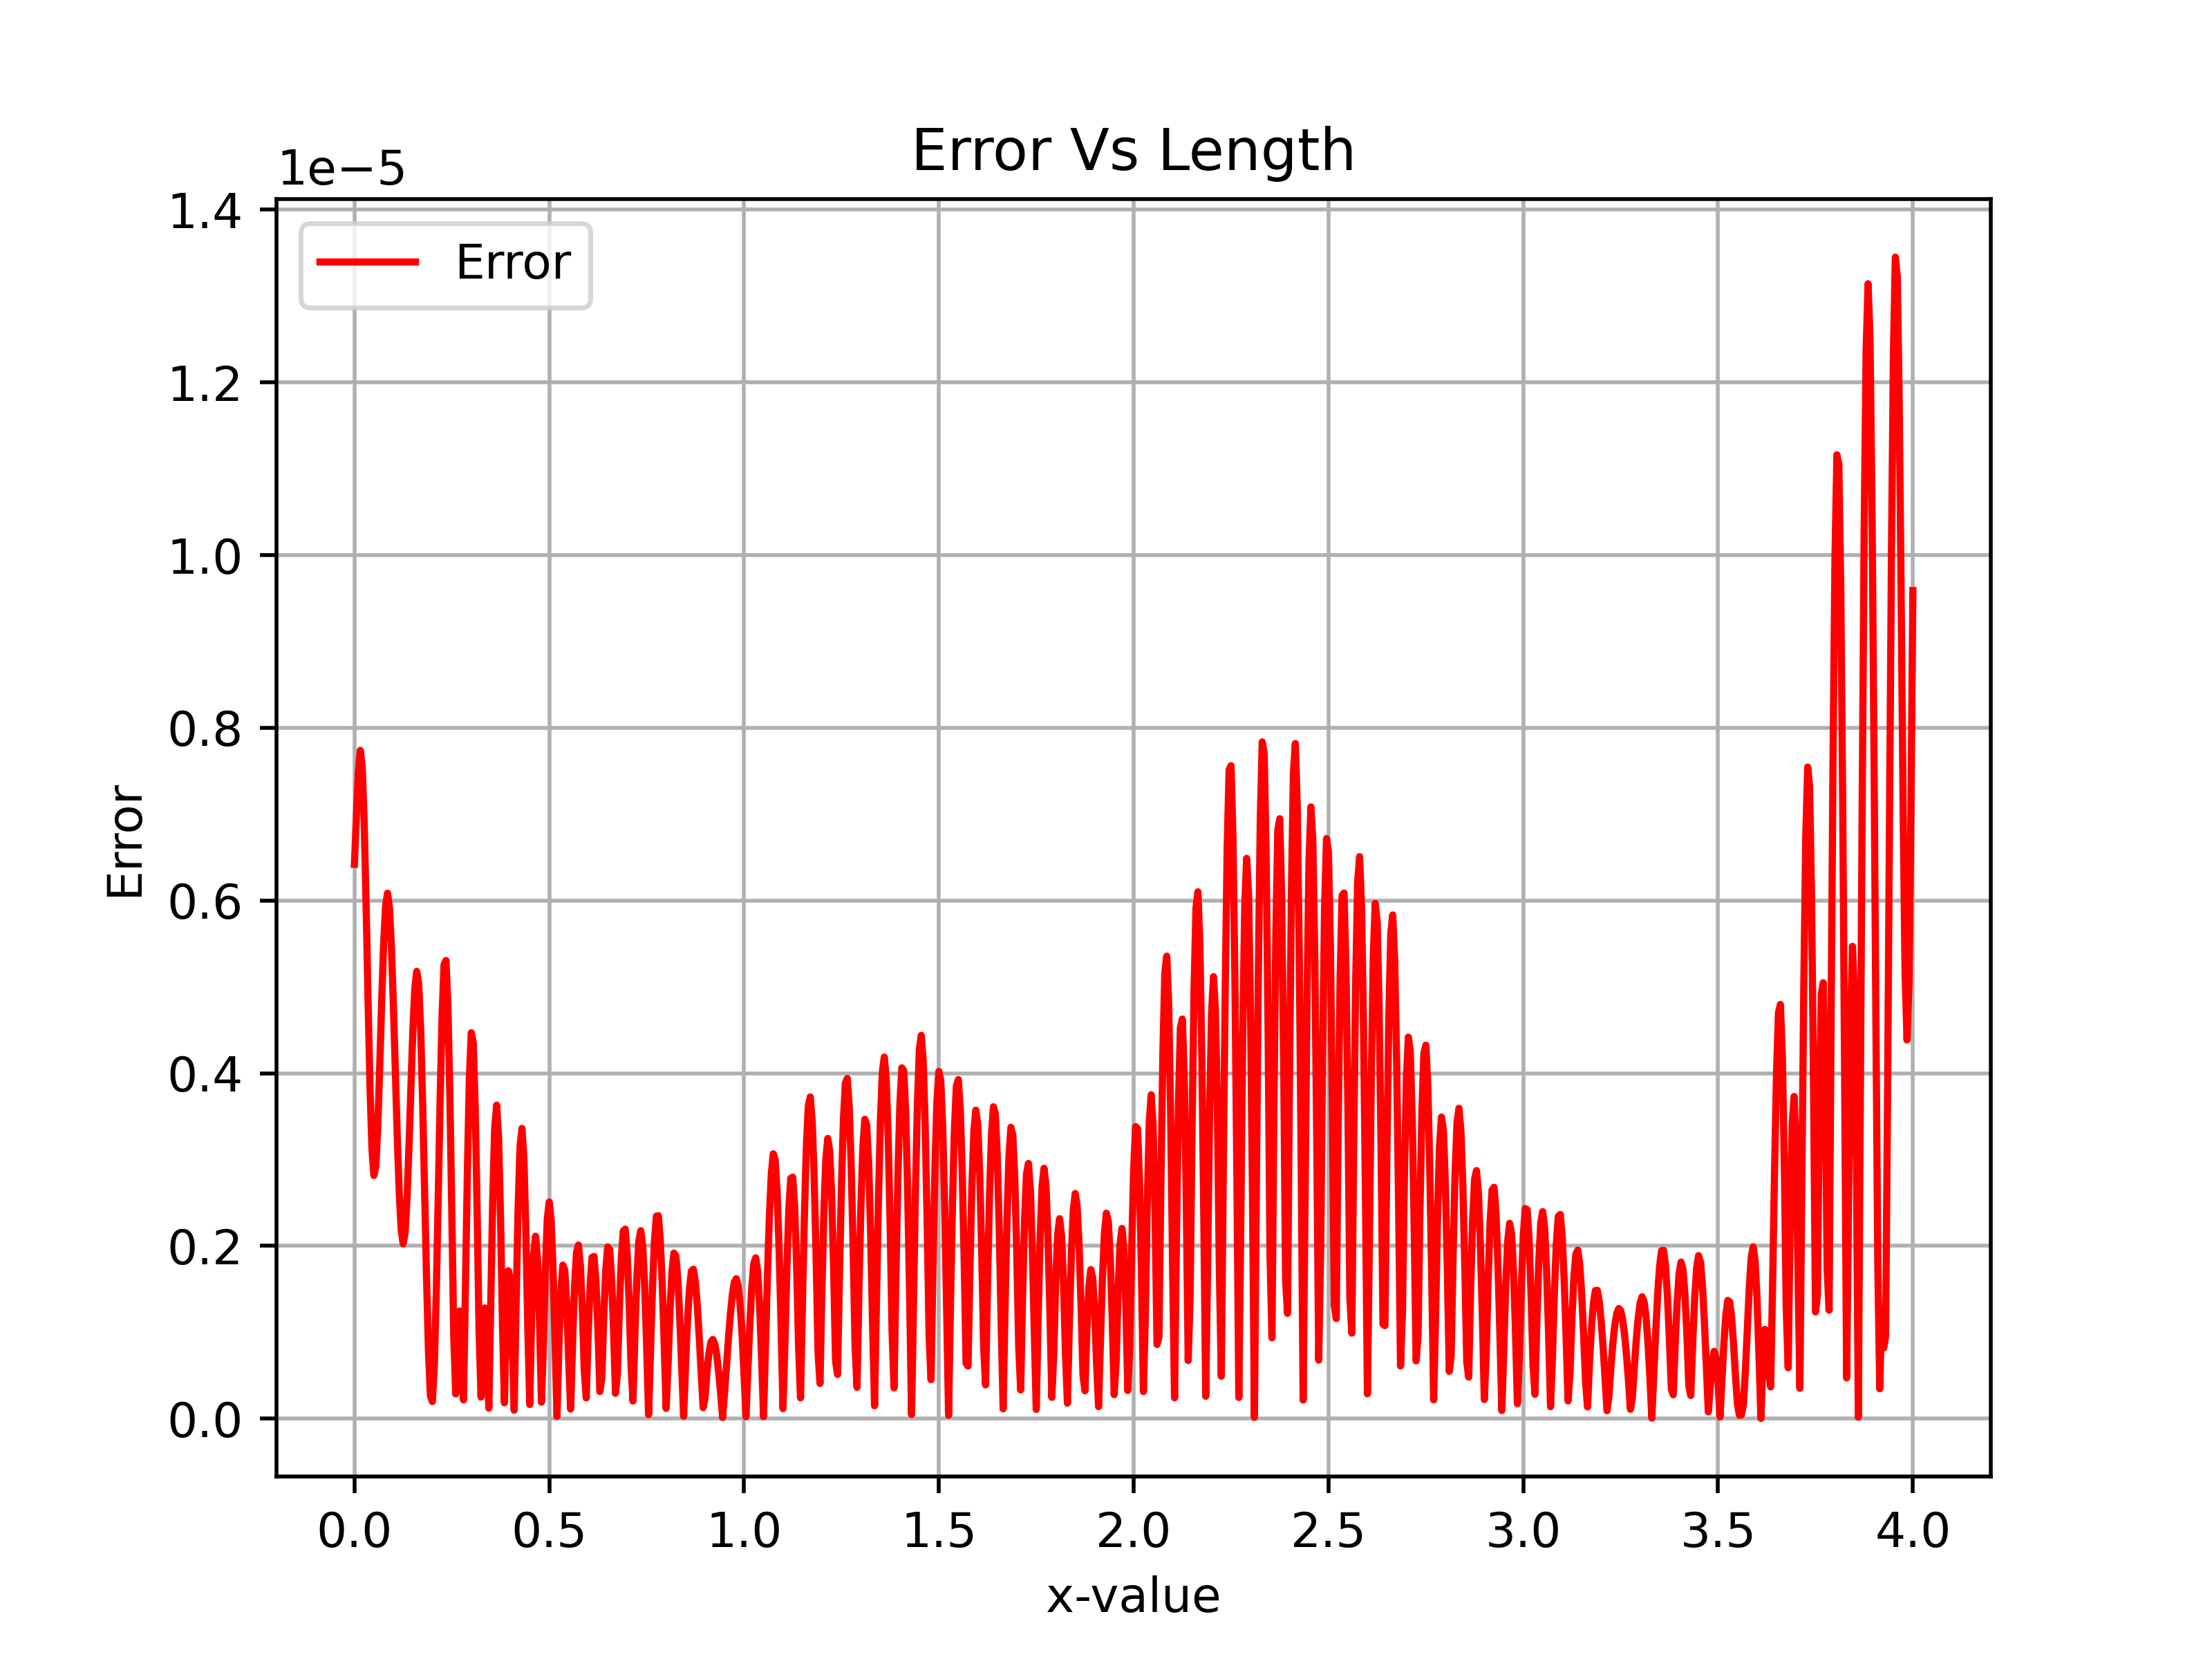
\includegraphics[scale=\size]{deptherr4.png}
\\~\\for hidden layers of depth $3$, the neural network output and analytical solution,
\\~\\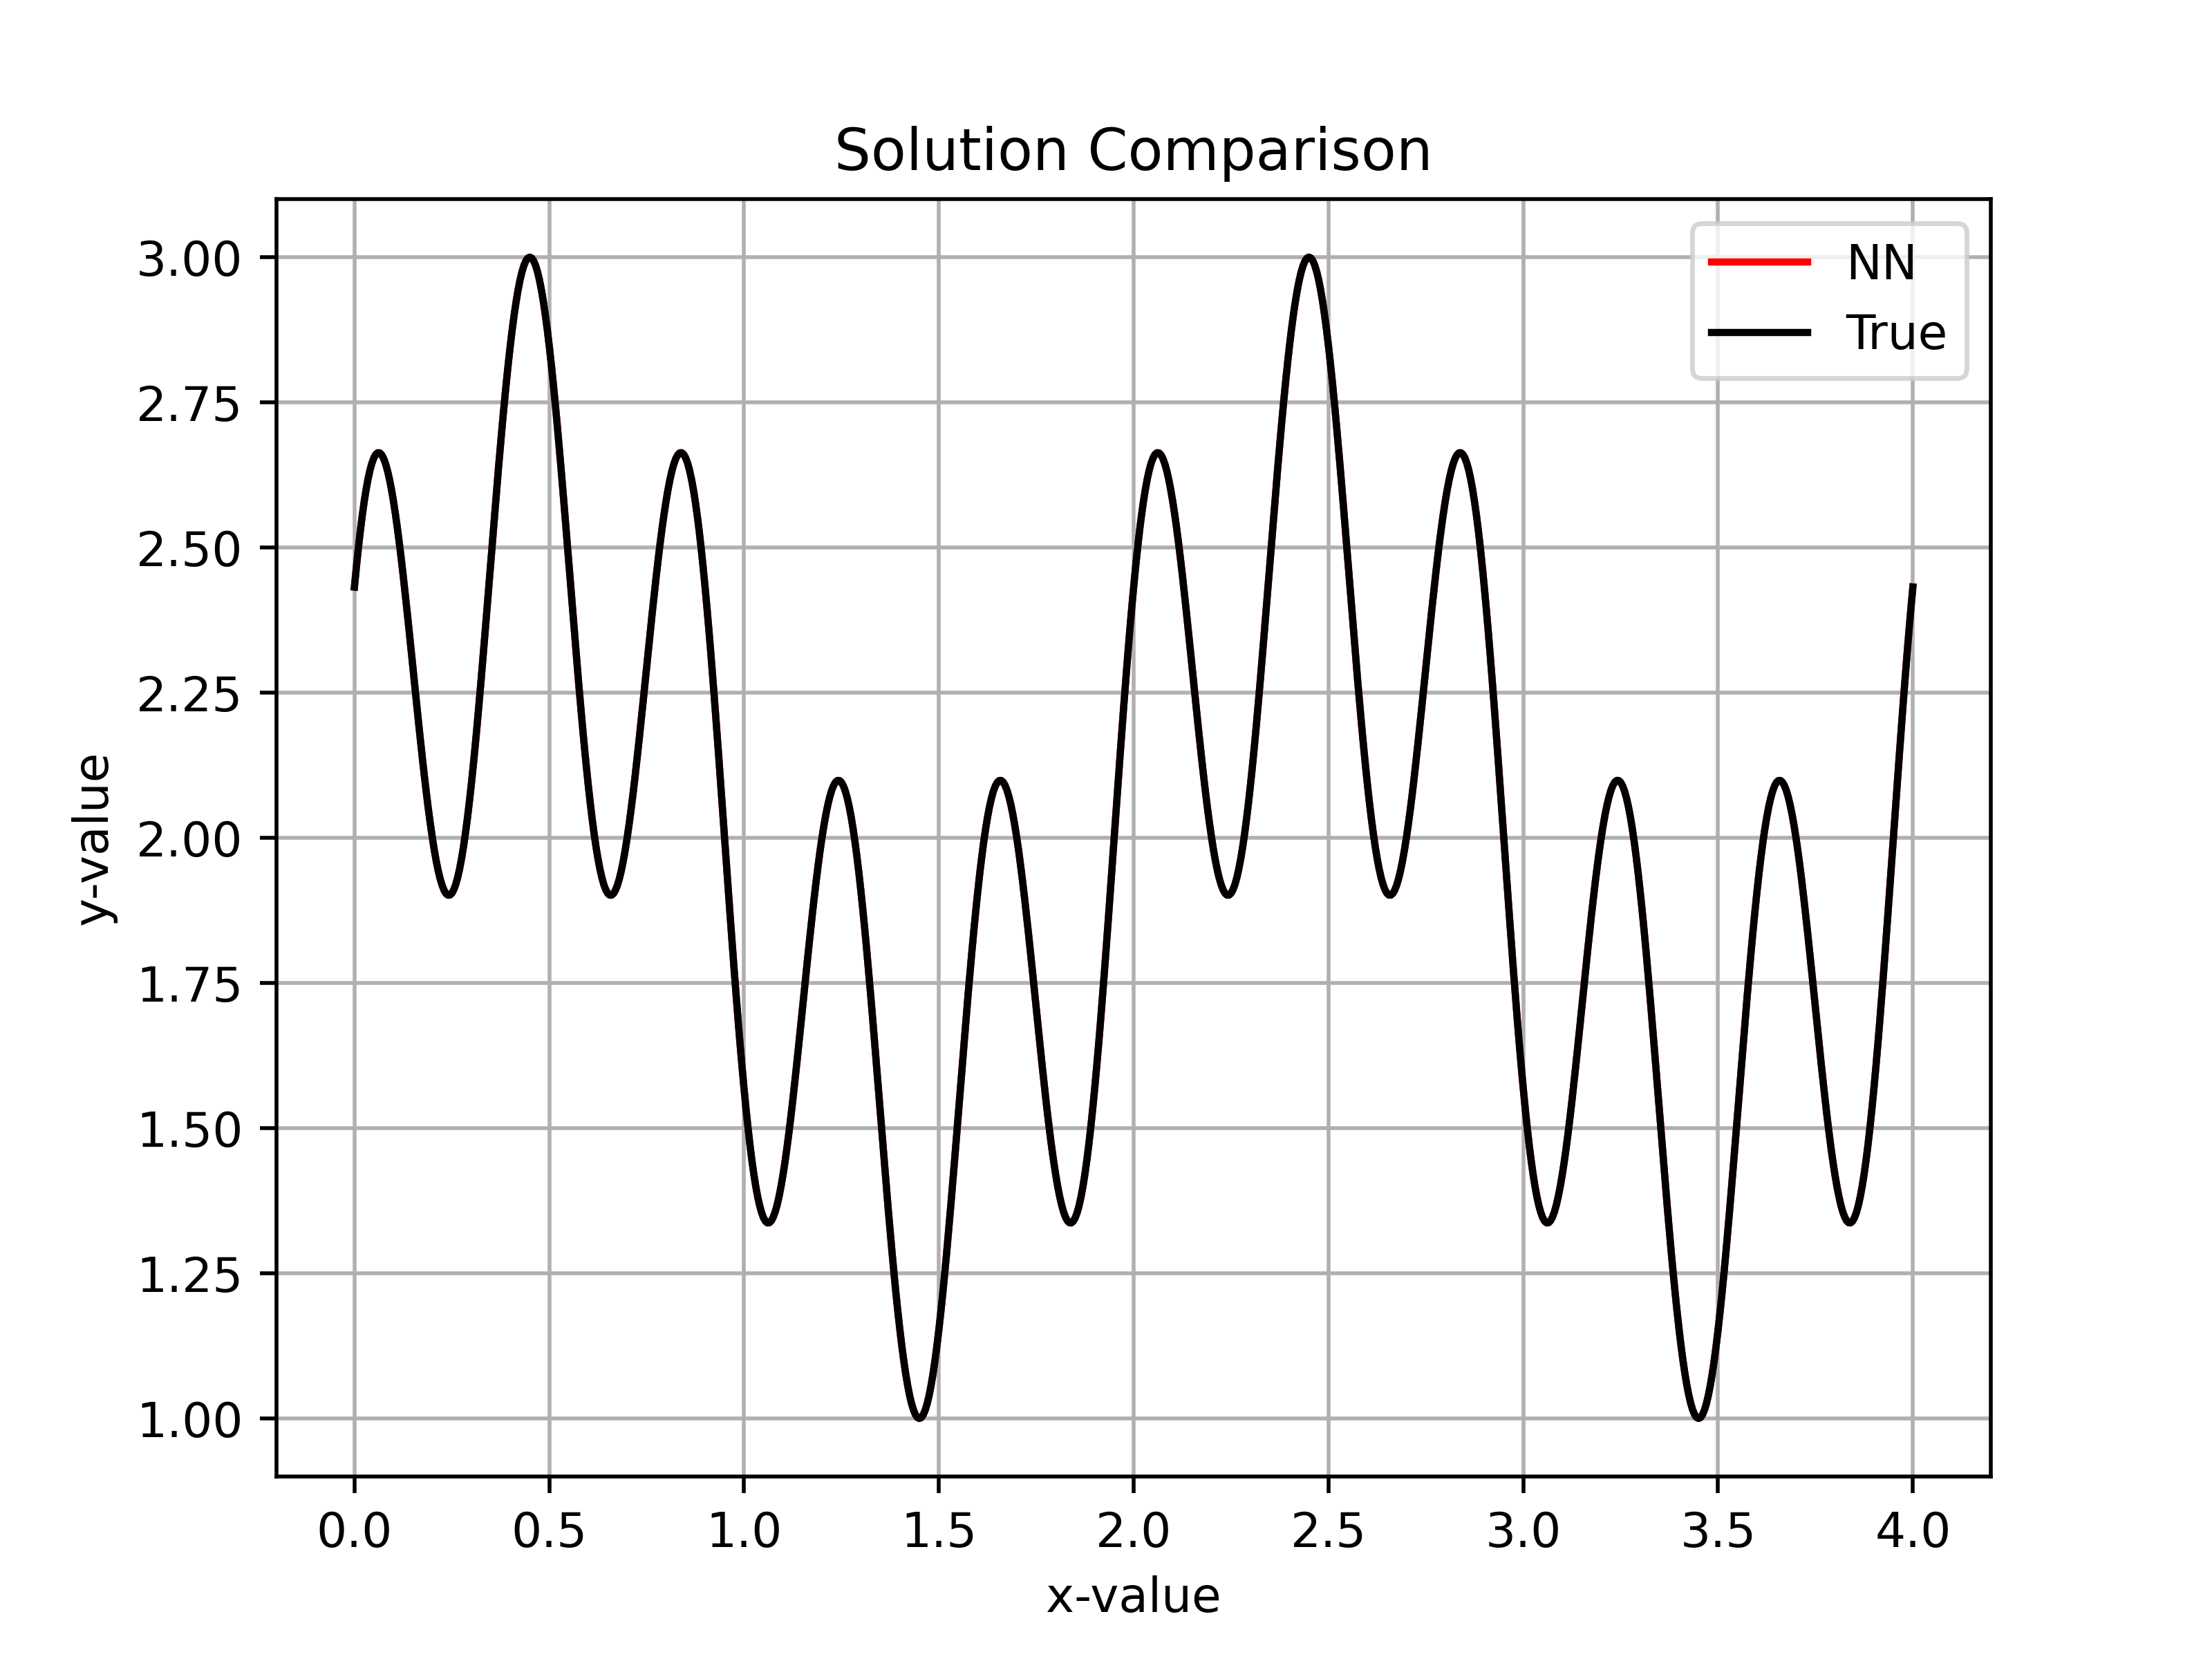
\includegraphics[scale=\size]{depthsol3.png}
\\~\\The corresponding error along the length of the domain,
\\~\\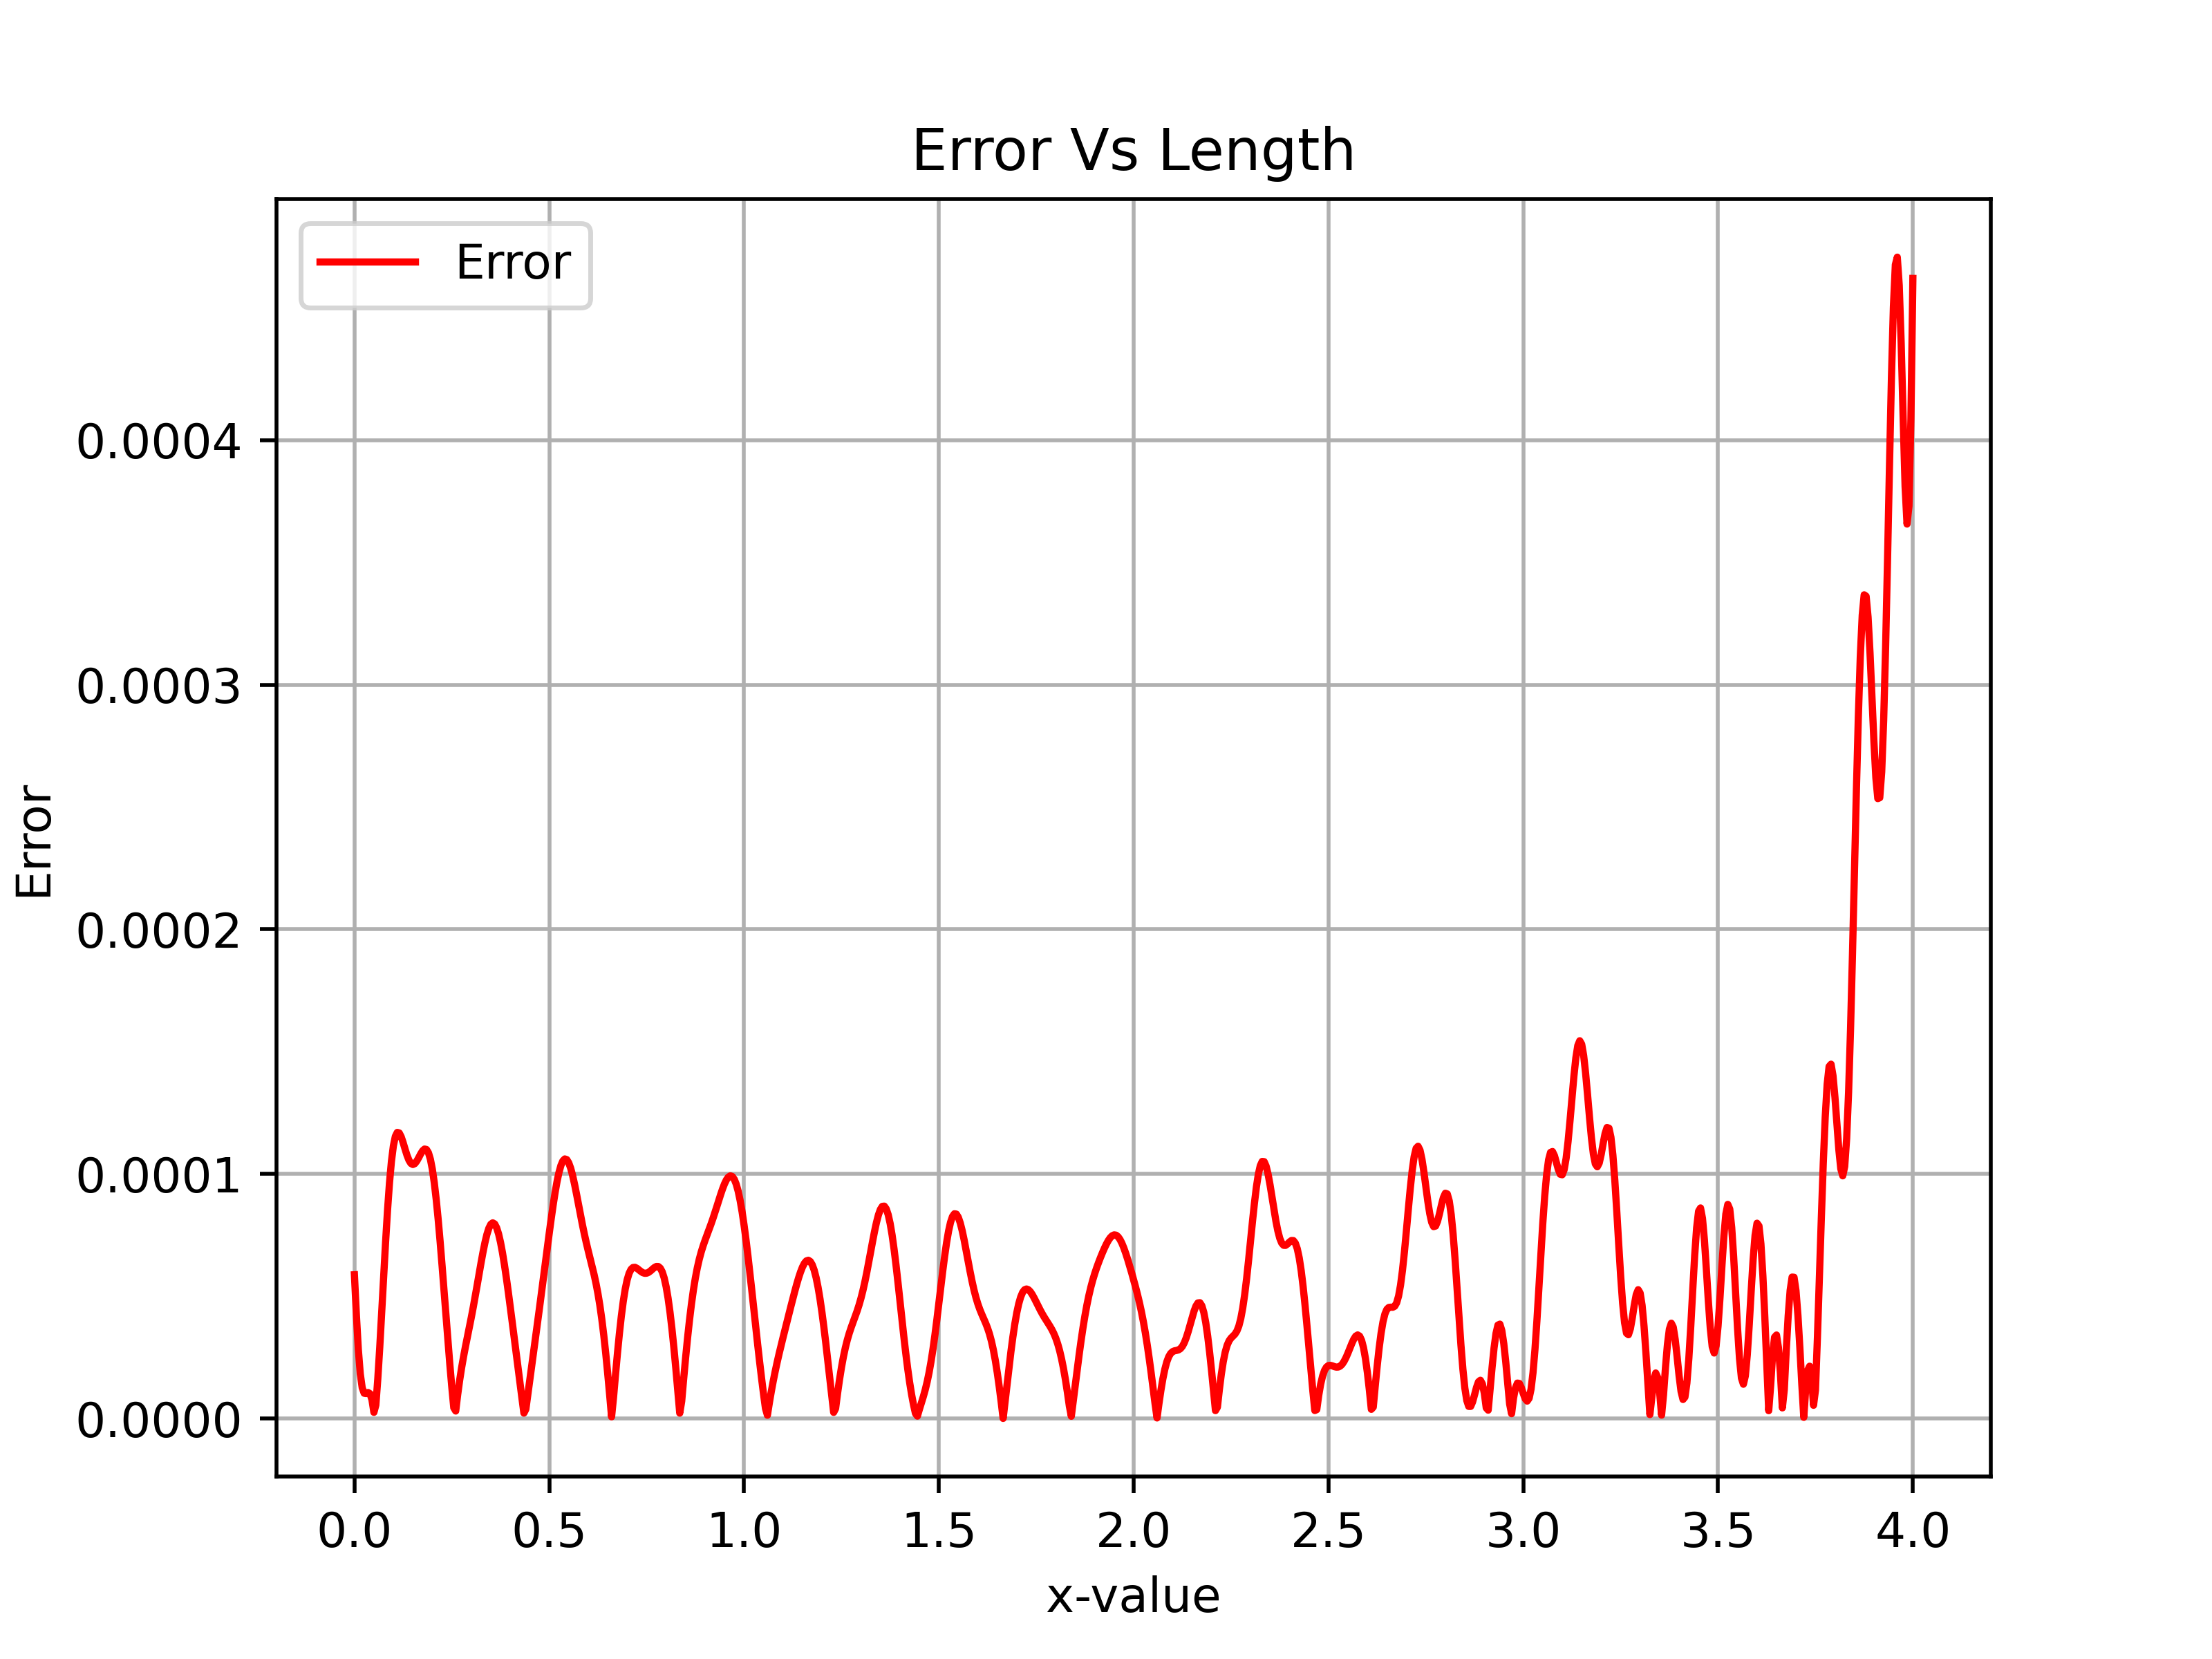
\includegraphics[scale=\size]{deptherr3.png}
\\~\\for hidden layers of depth $2$, the neural network output and analytical solution,
\\~\\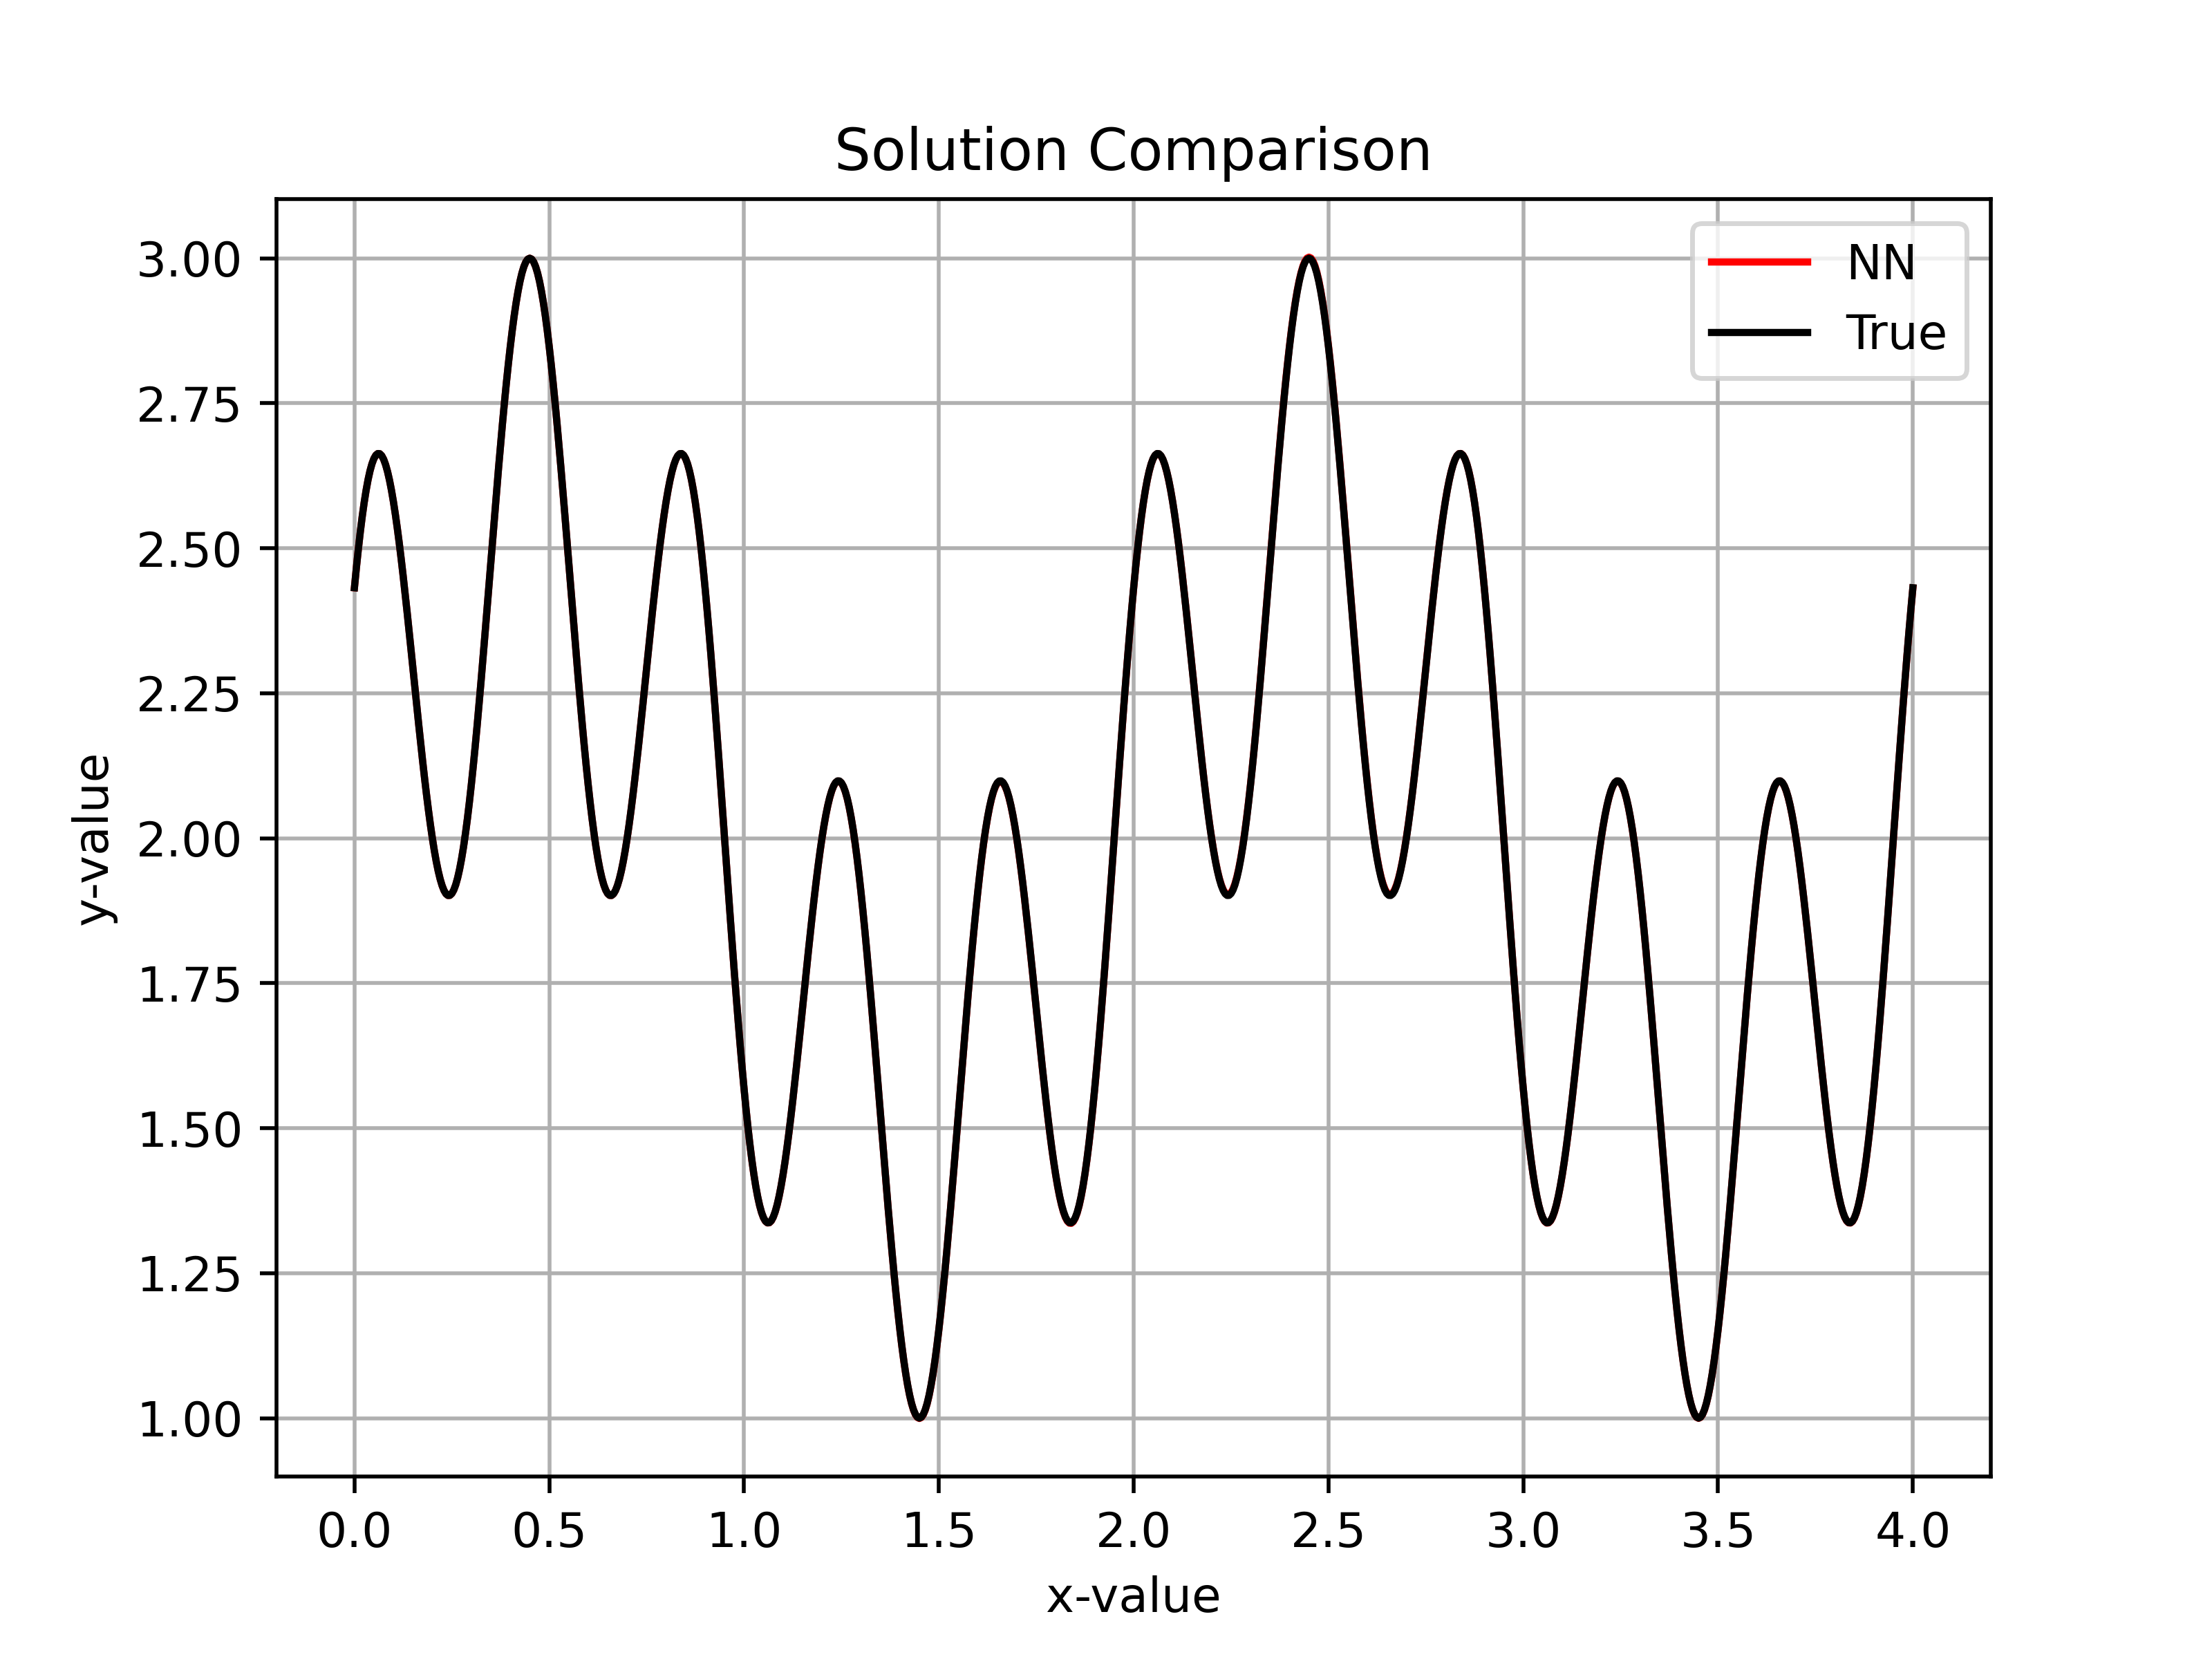
\includegraphics[scale=\size]{depthsol2.png}
\\~\\The corresponding error along the length of the domain,
\\~\\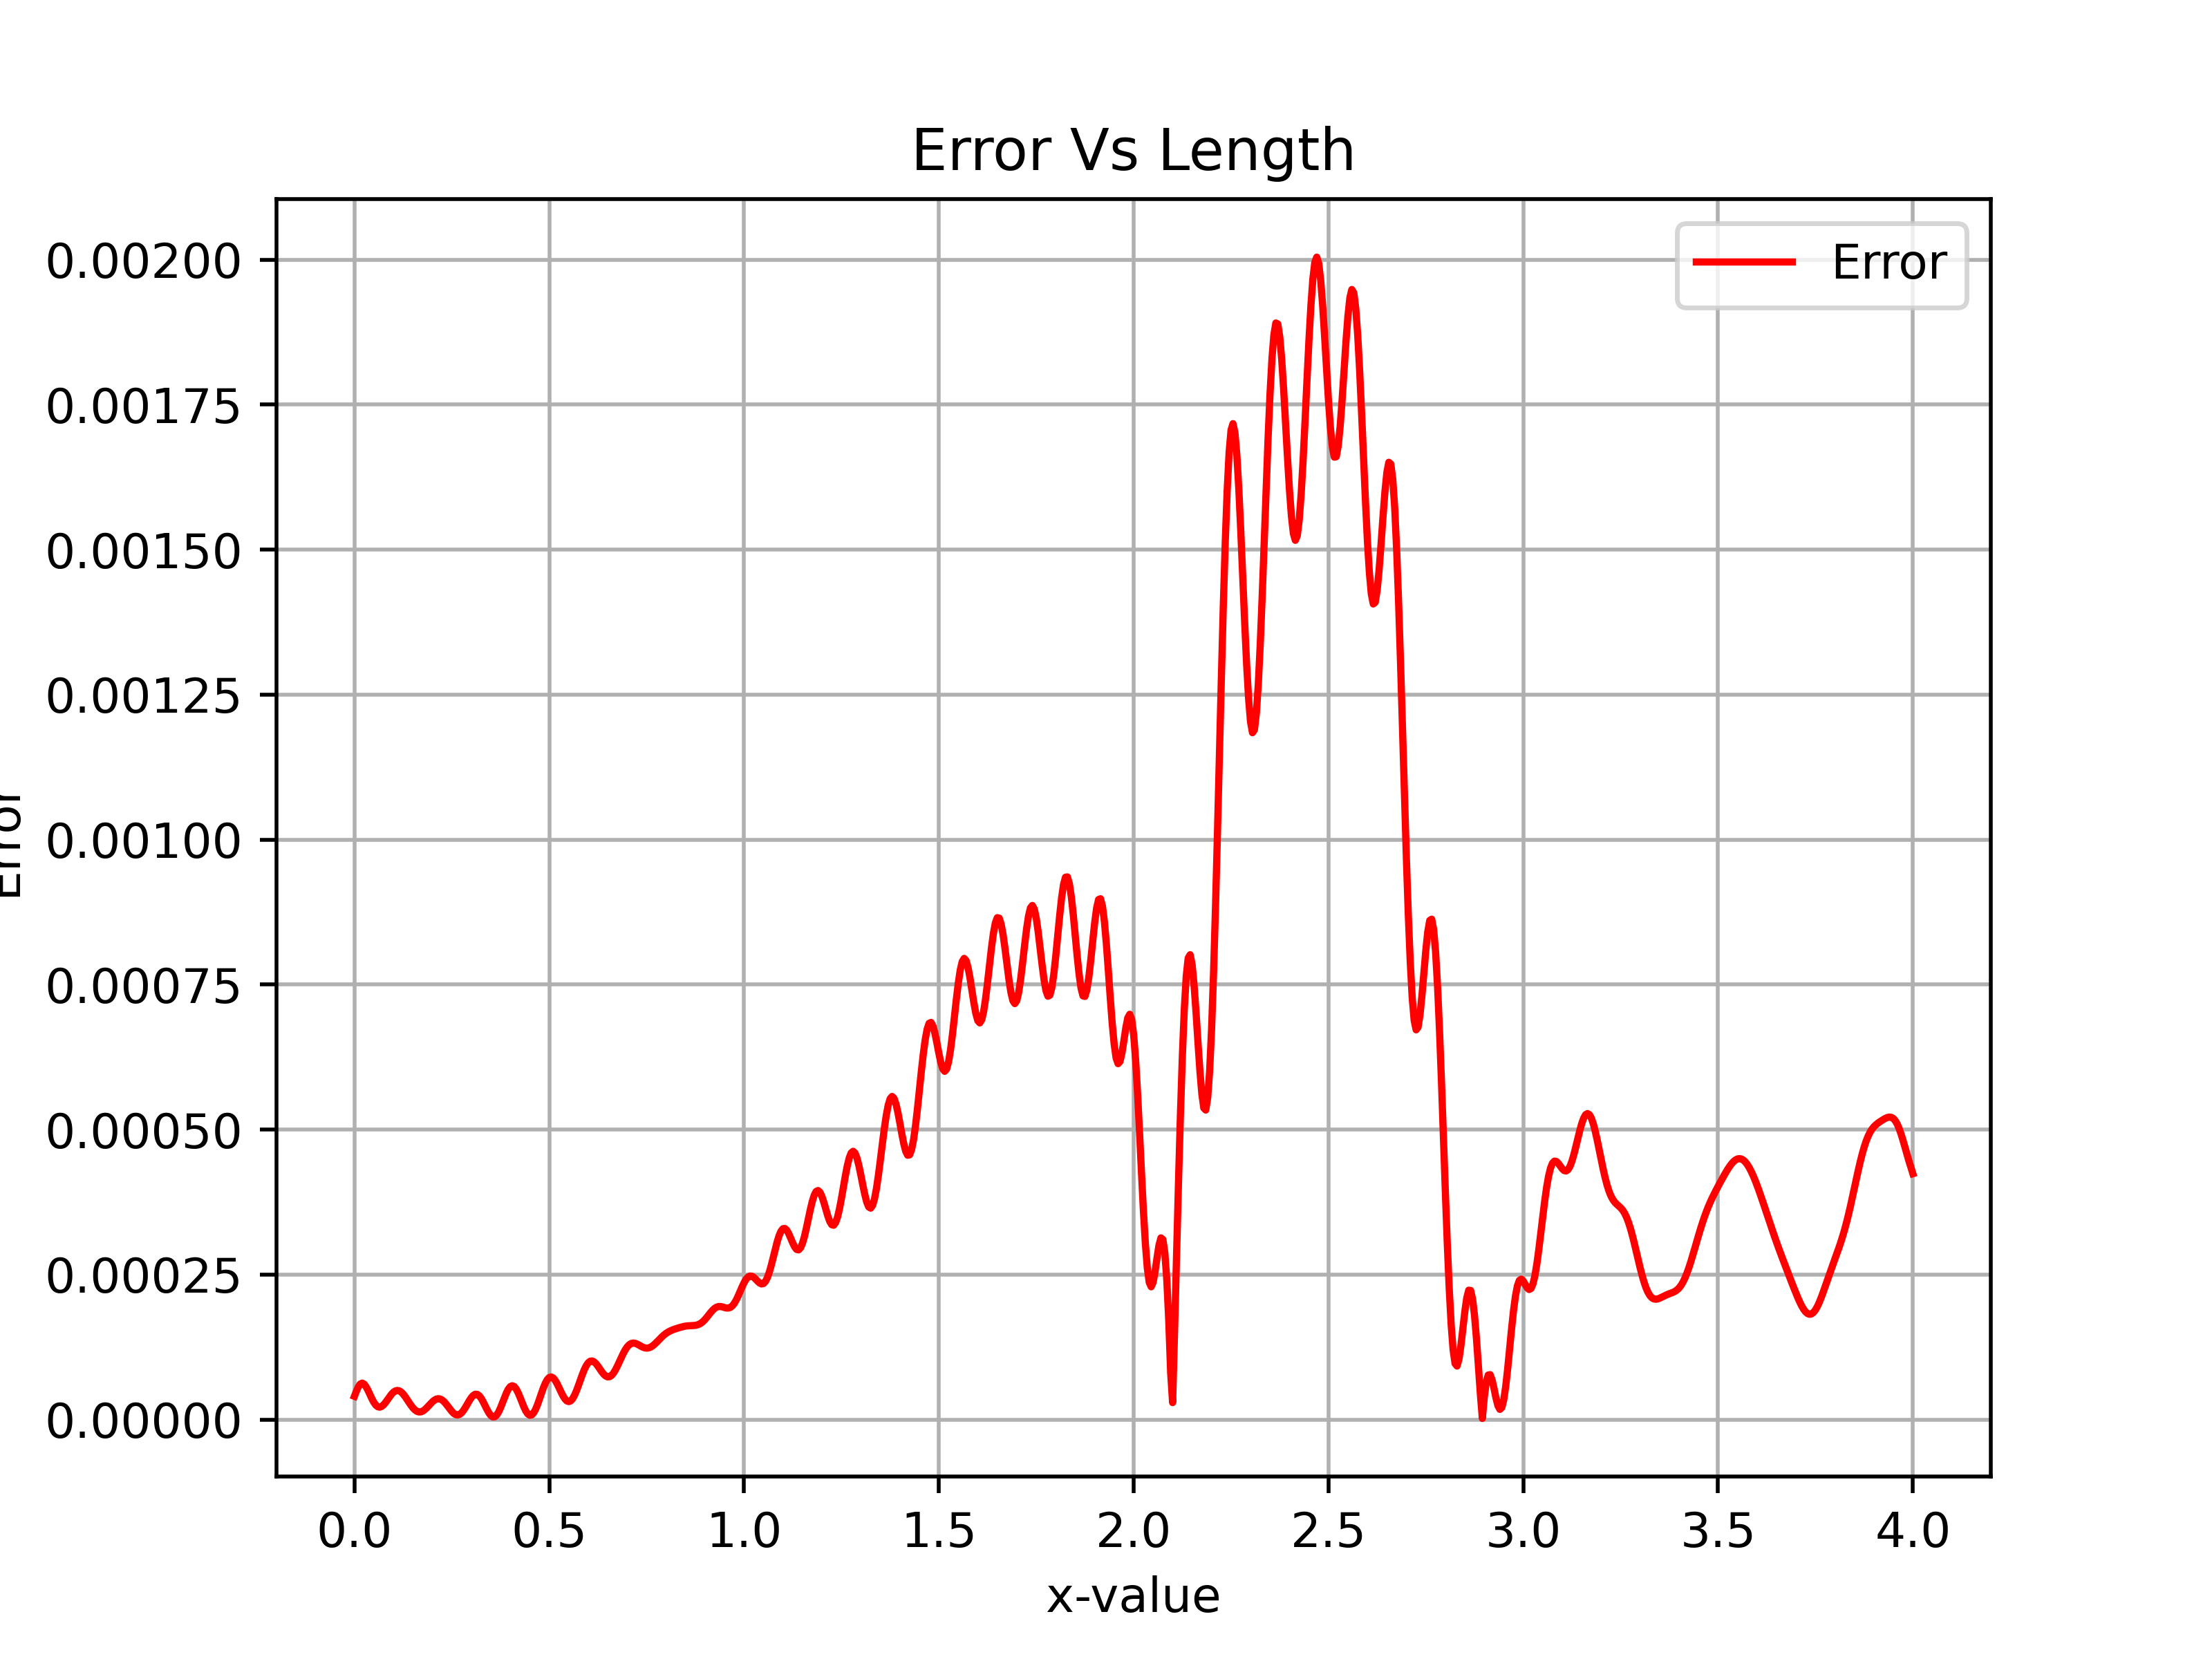
\includegraphics[scale=\size]{deptherr2.png}
\\~\\for hidden layers of depth $1$, the neural network output and analytical solution,
\\~\\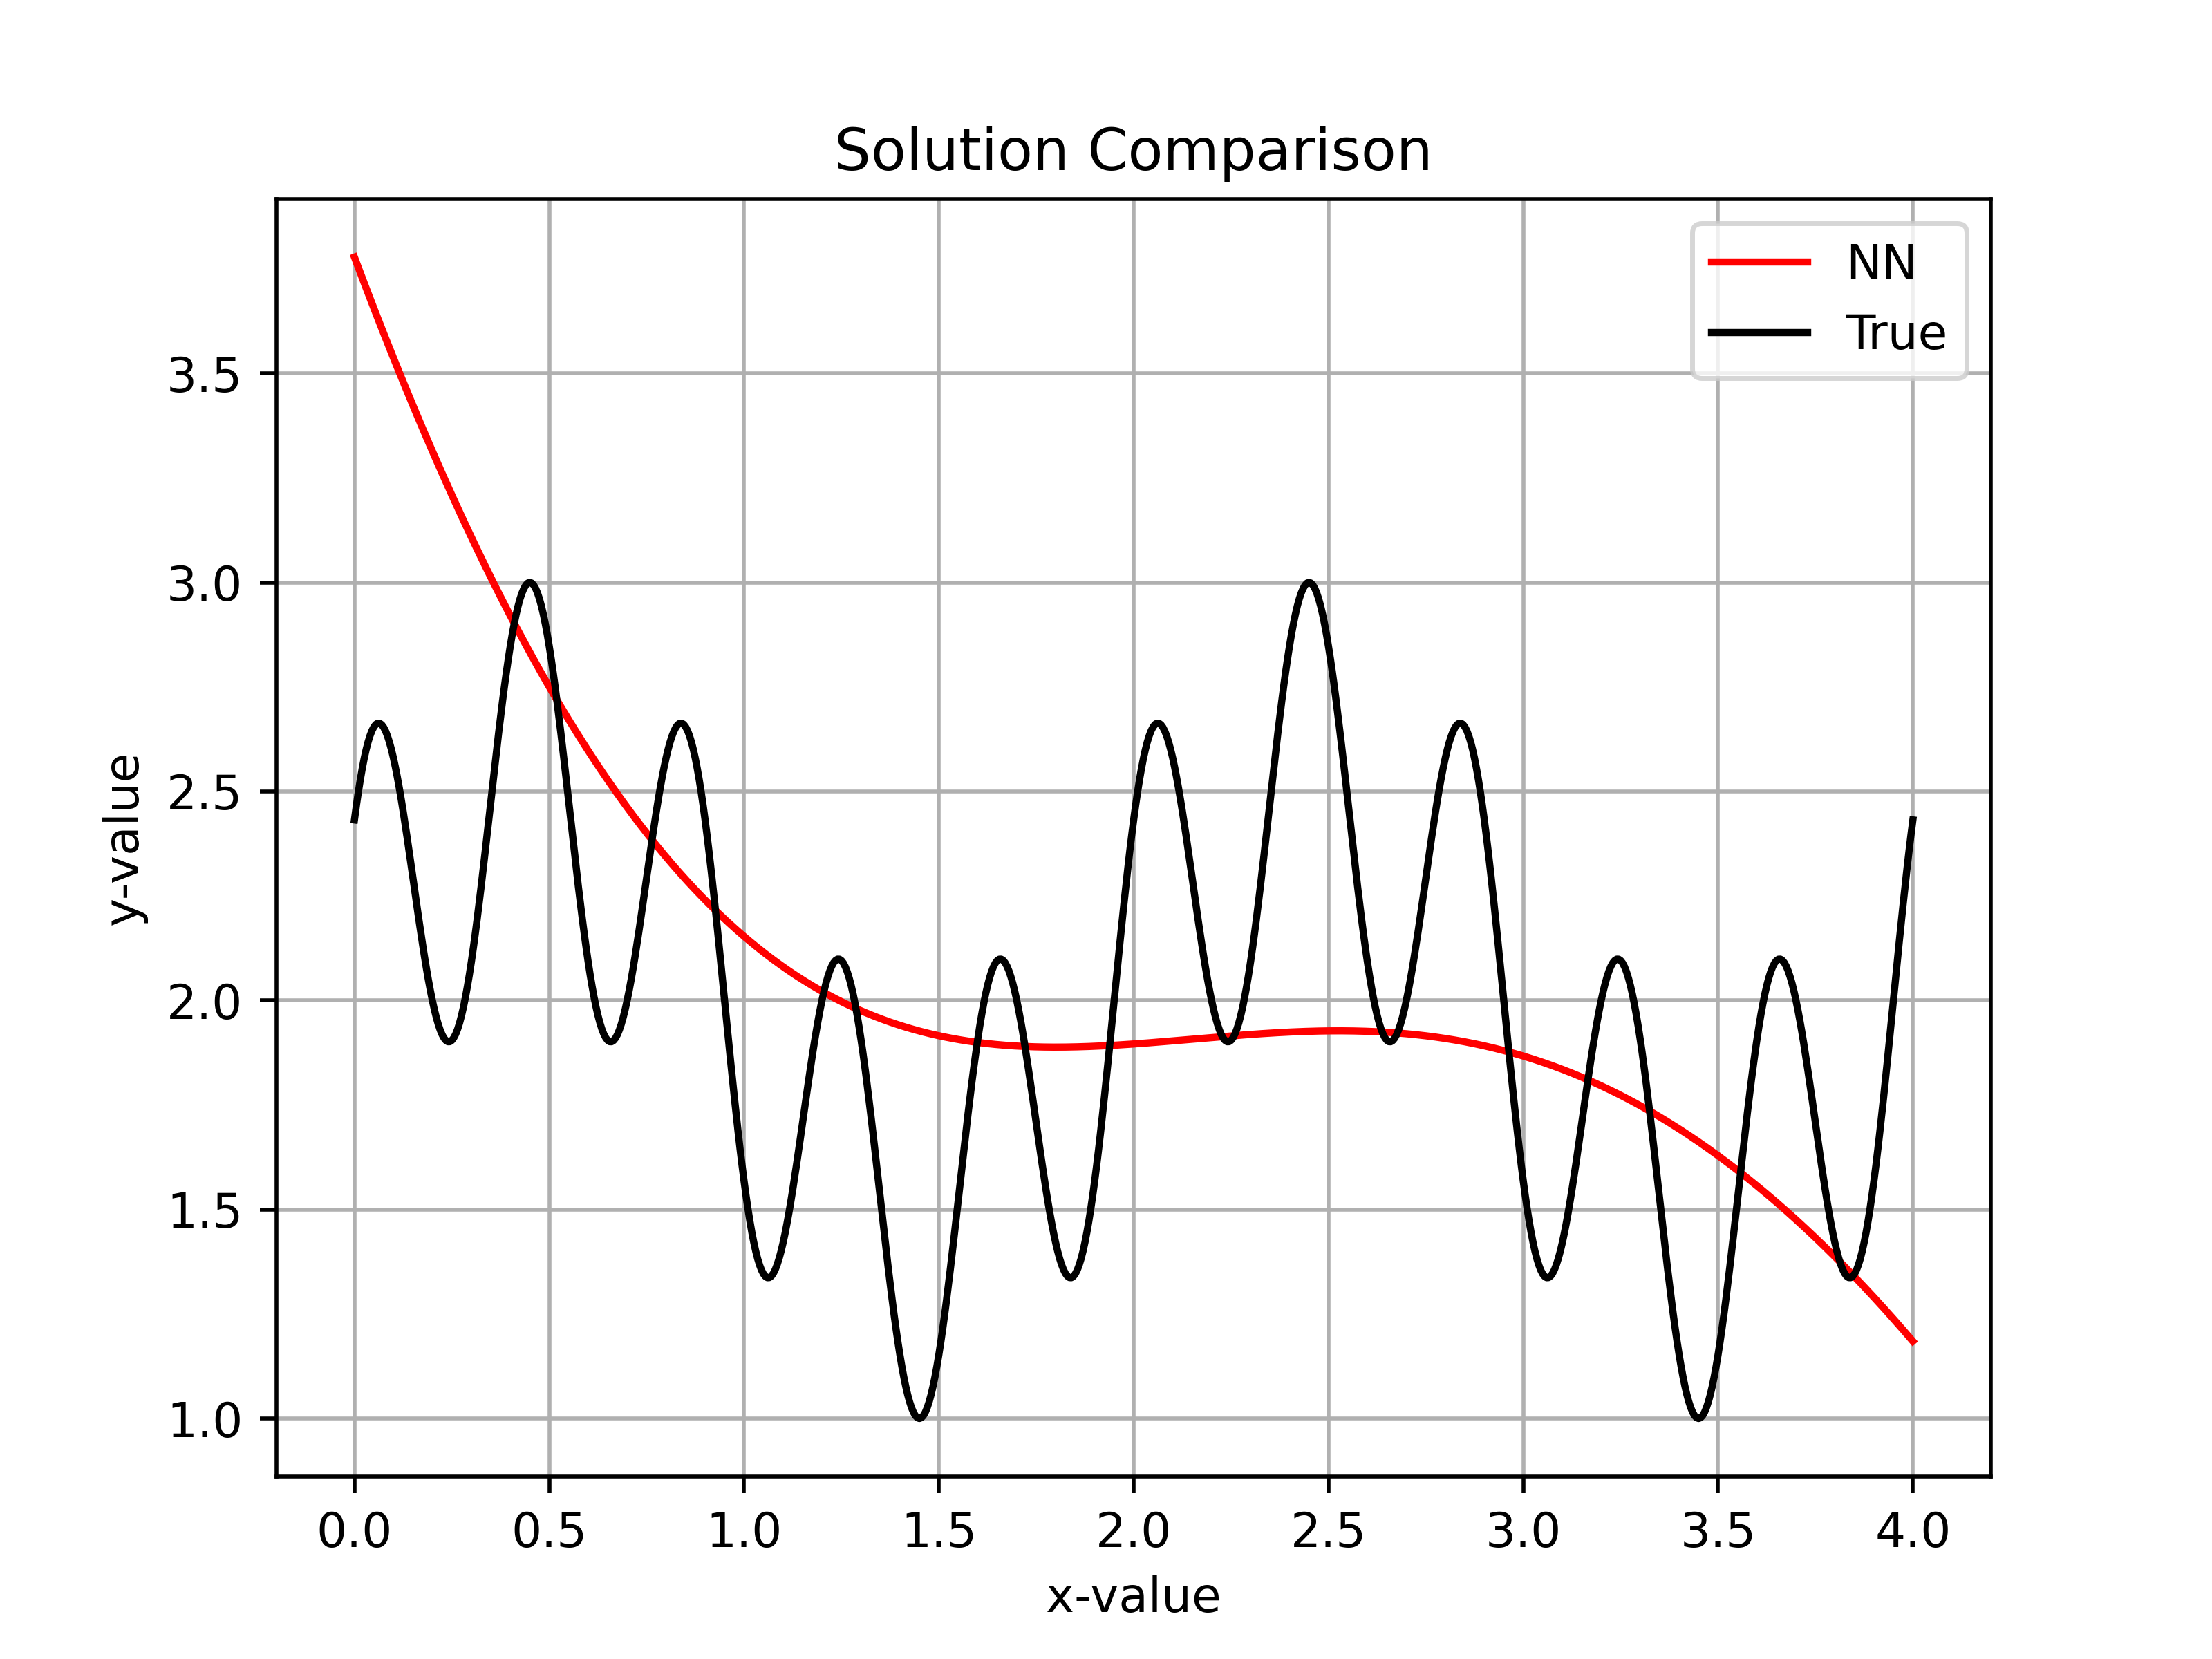
\includegraphics[scale=\size]{depthsol1.png}
\\~\\The corresponding error along the length of the domain,
\\~\\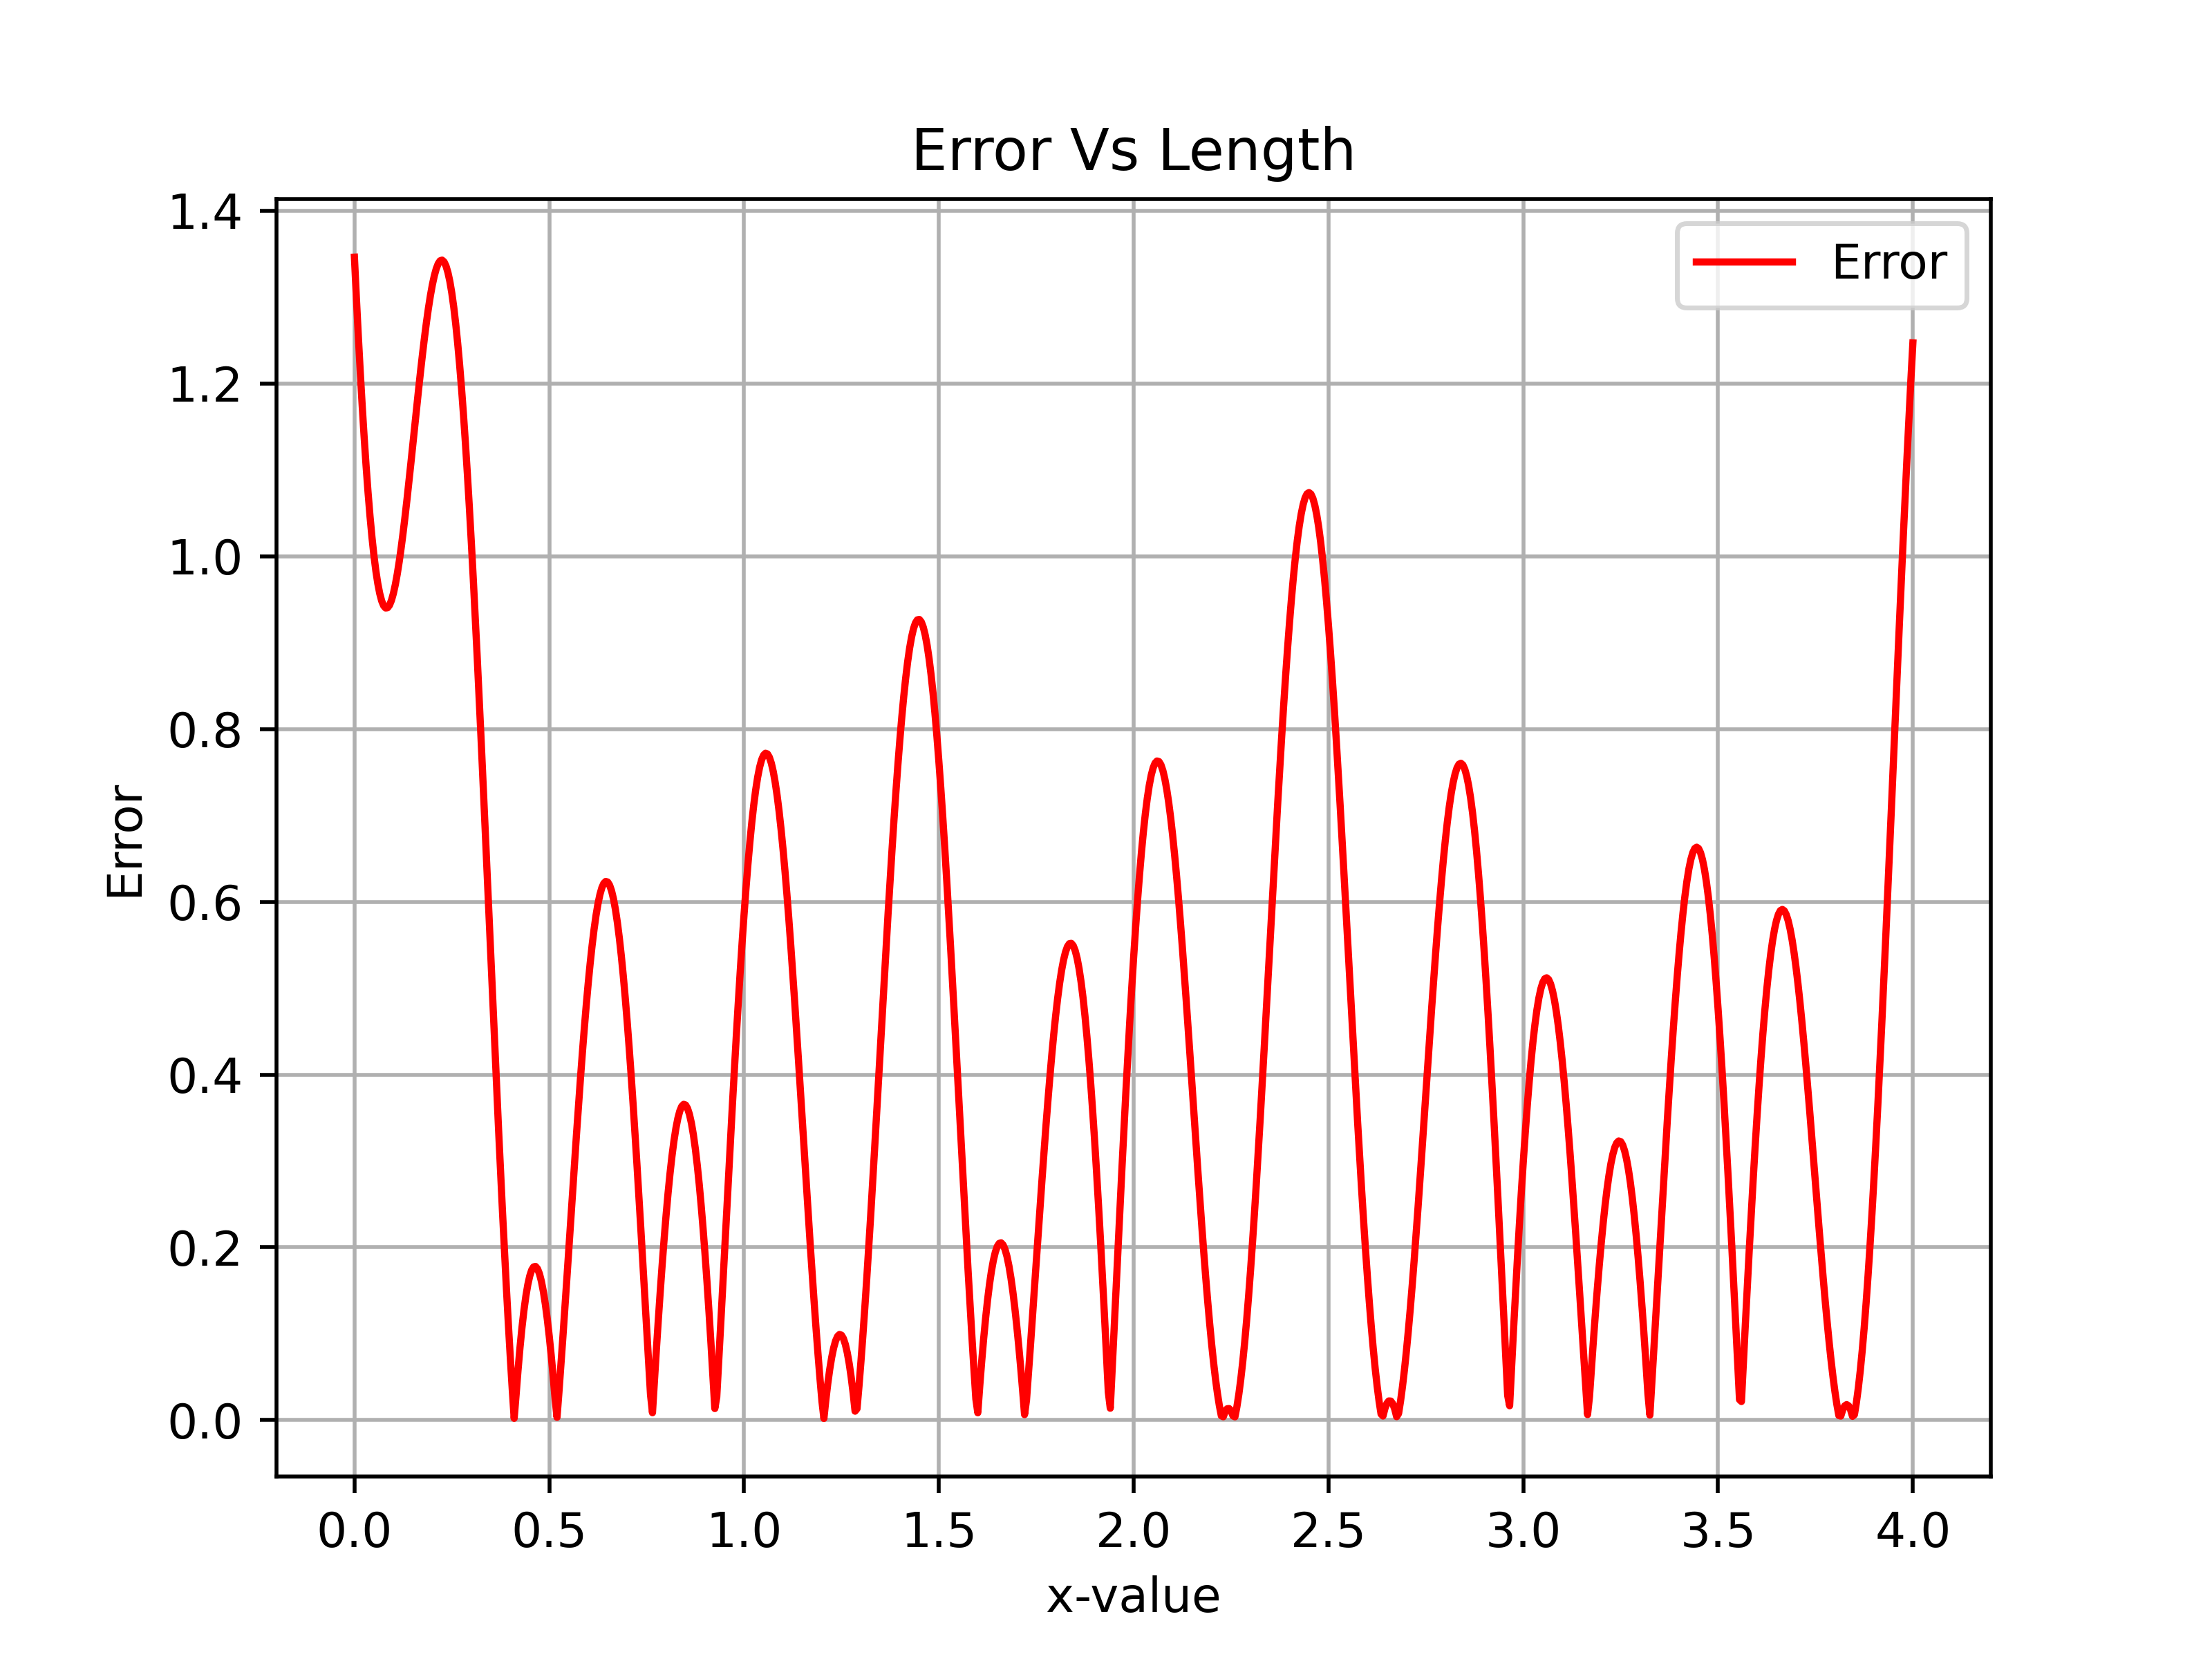
\includegraphics[scale=\size]{deptherr1.png}
\\~\\~\\The maximum error along the entire domain is collected and plotted against the corresponding Neural Network depth and is shown below,
\\~\\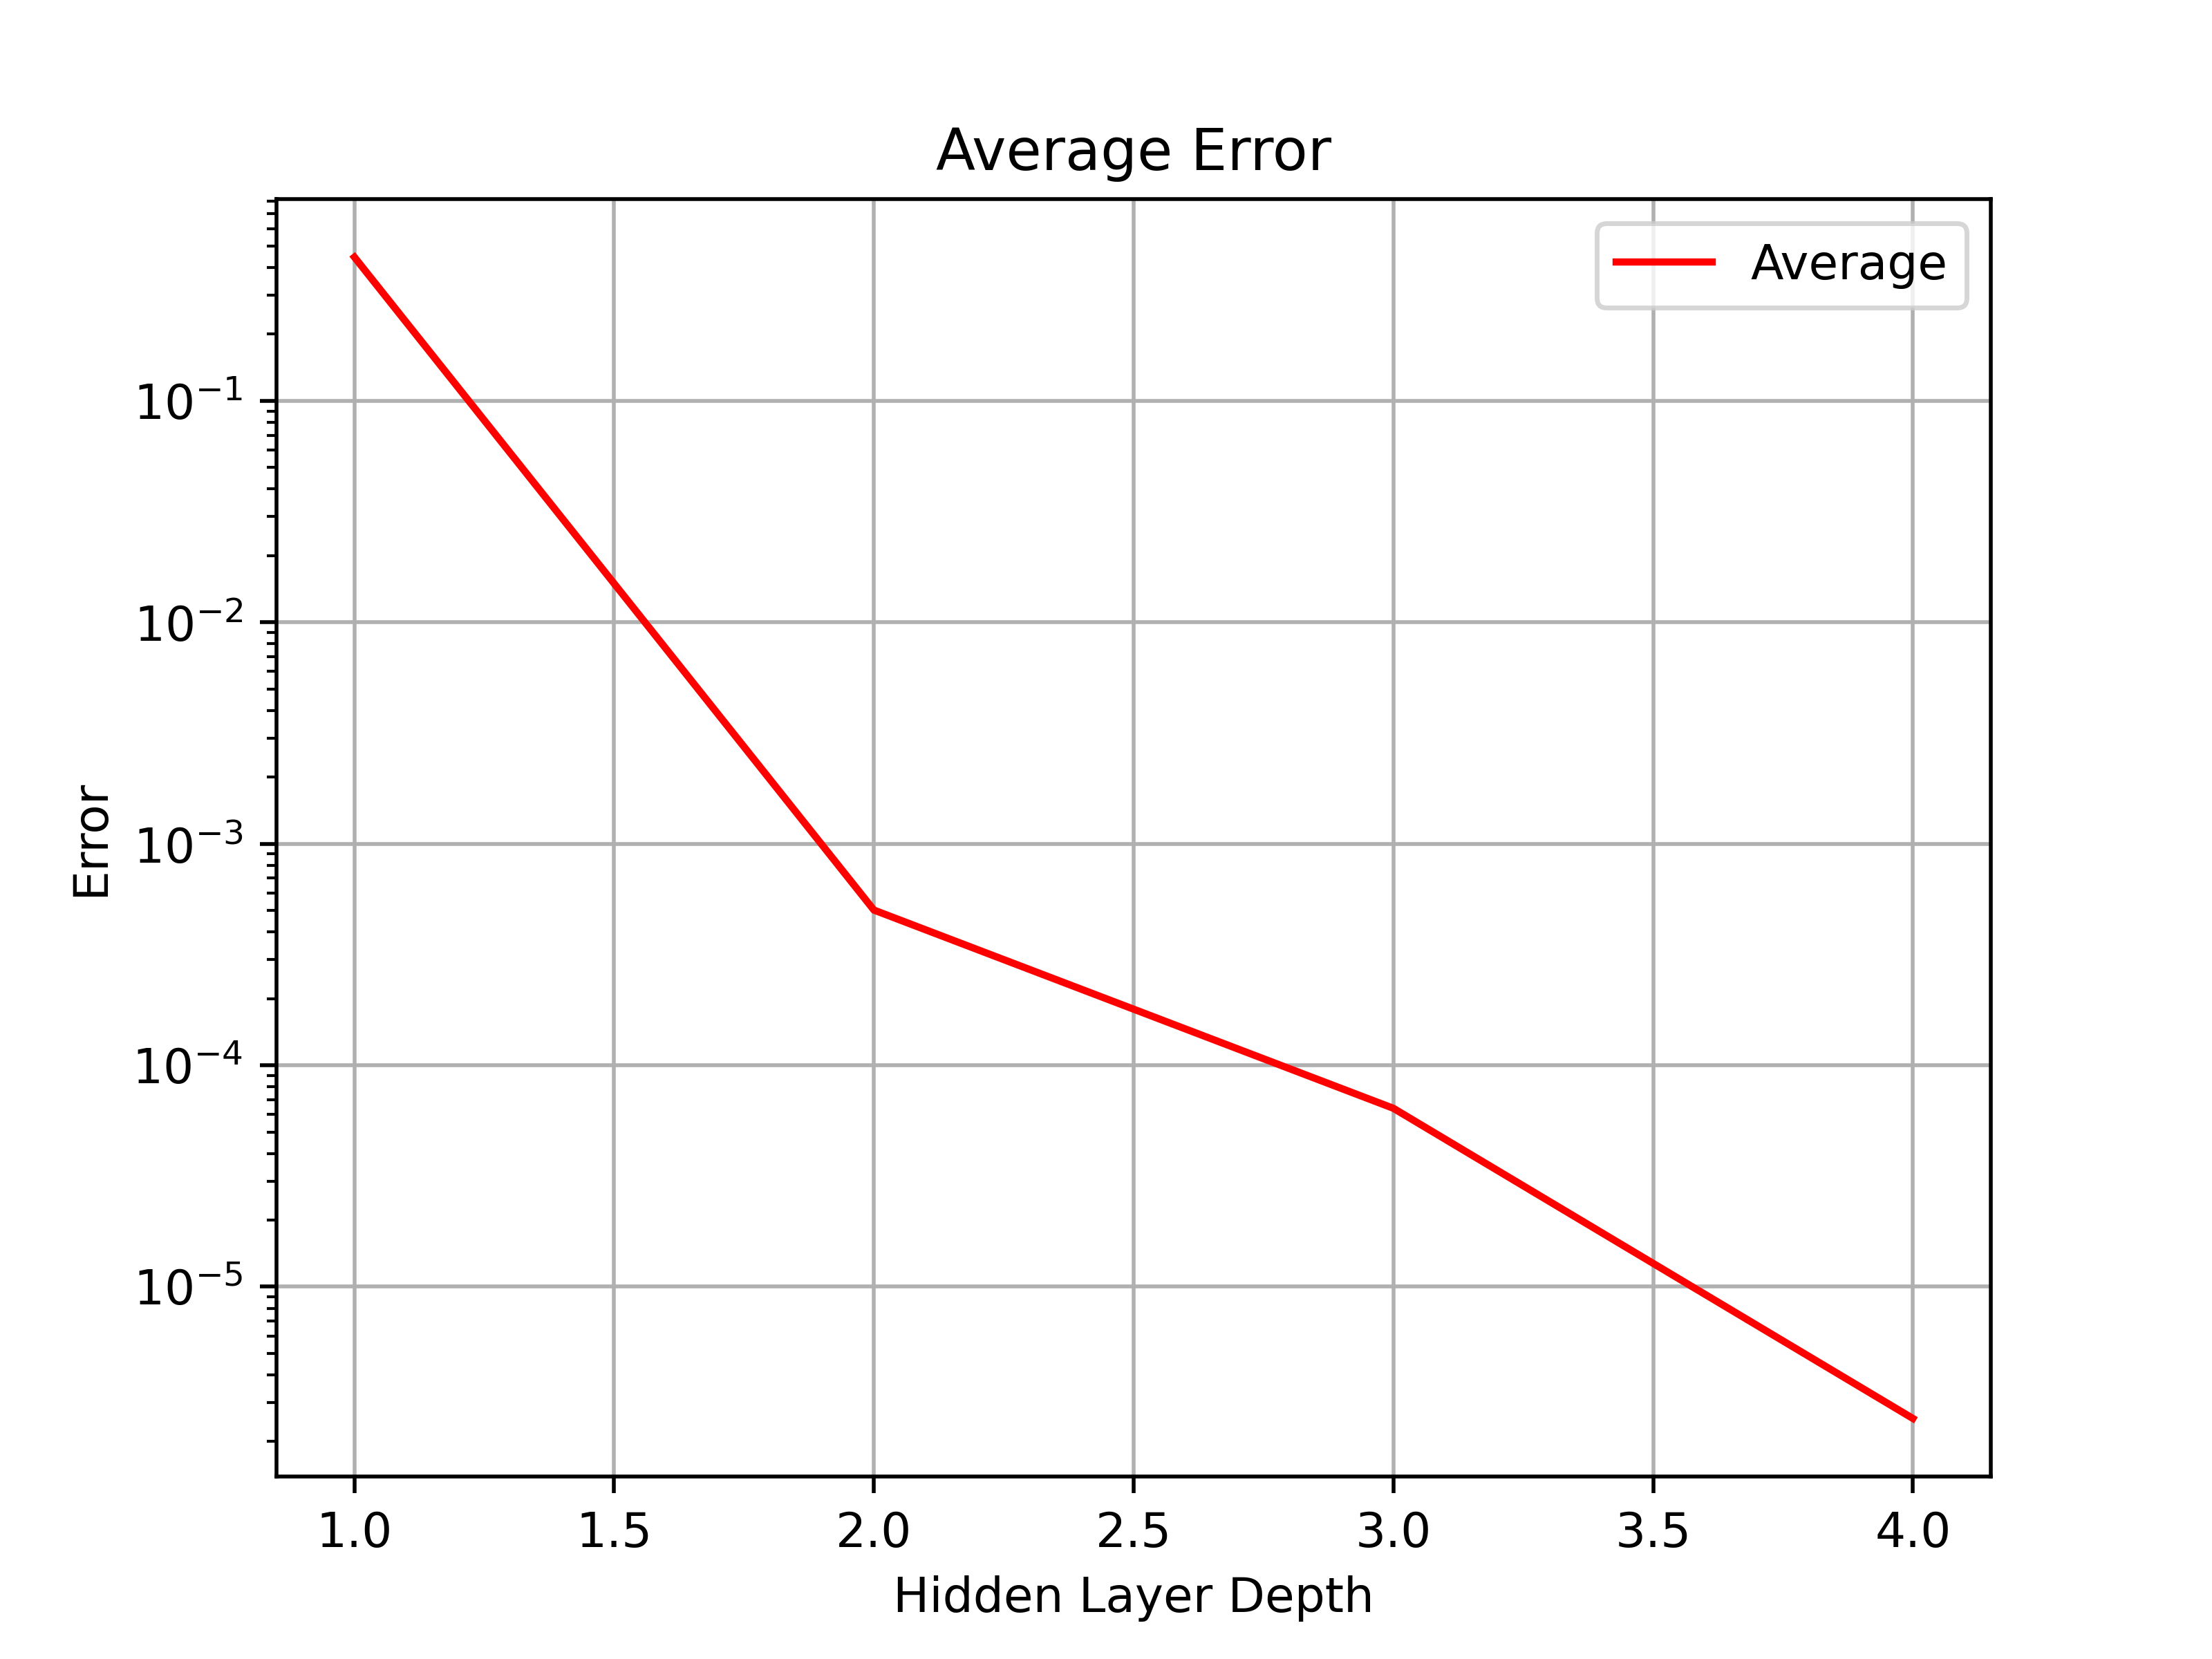
\includegraphics[scale=\size]{depthMean.png}
\\~\\The average error along the entire domain is shown below,
\\~\\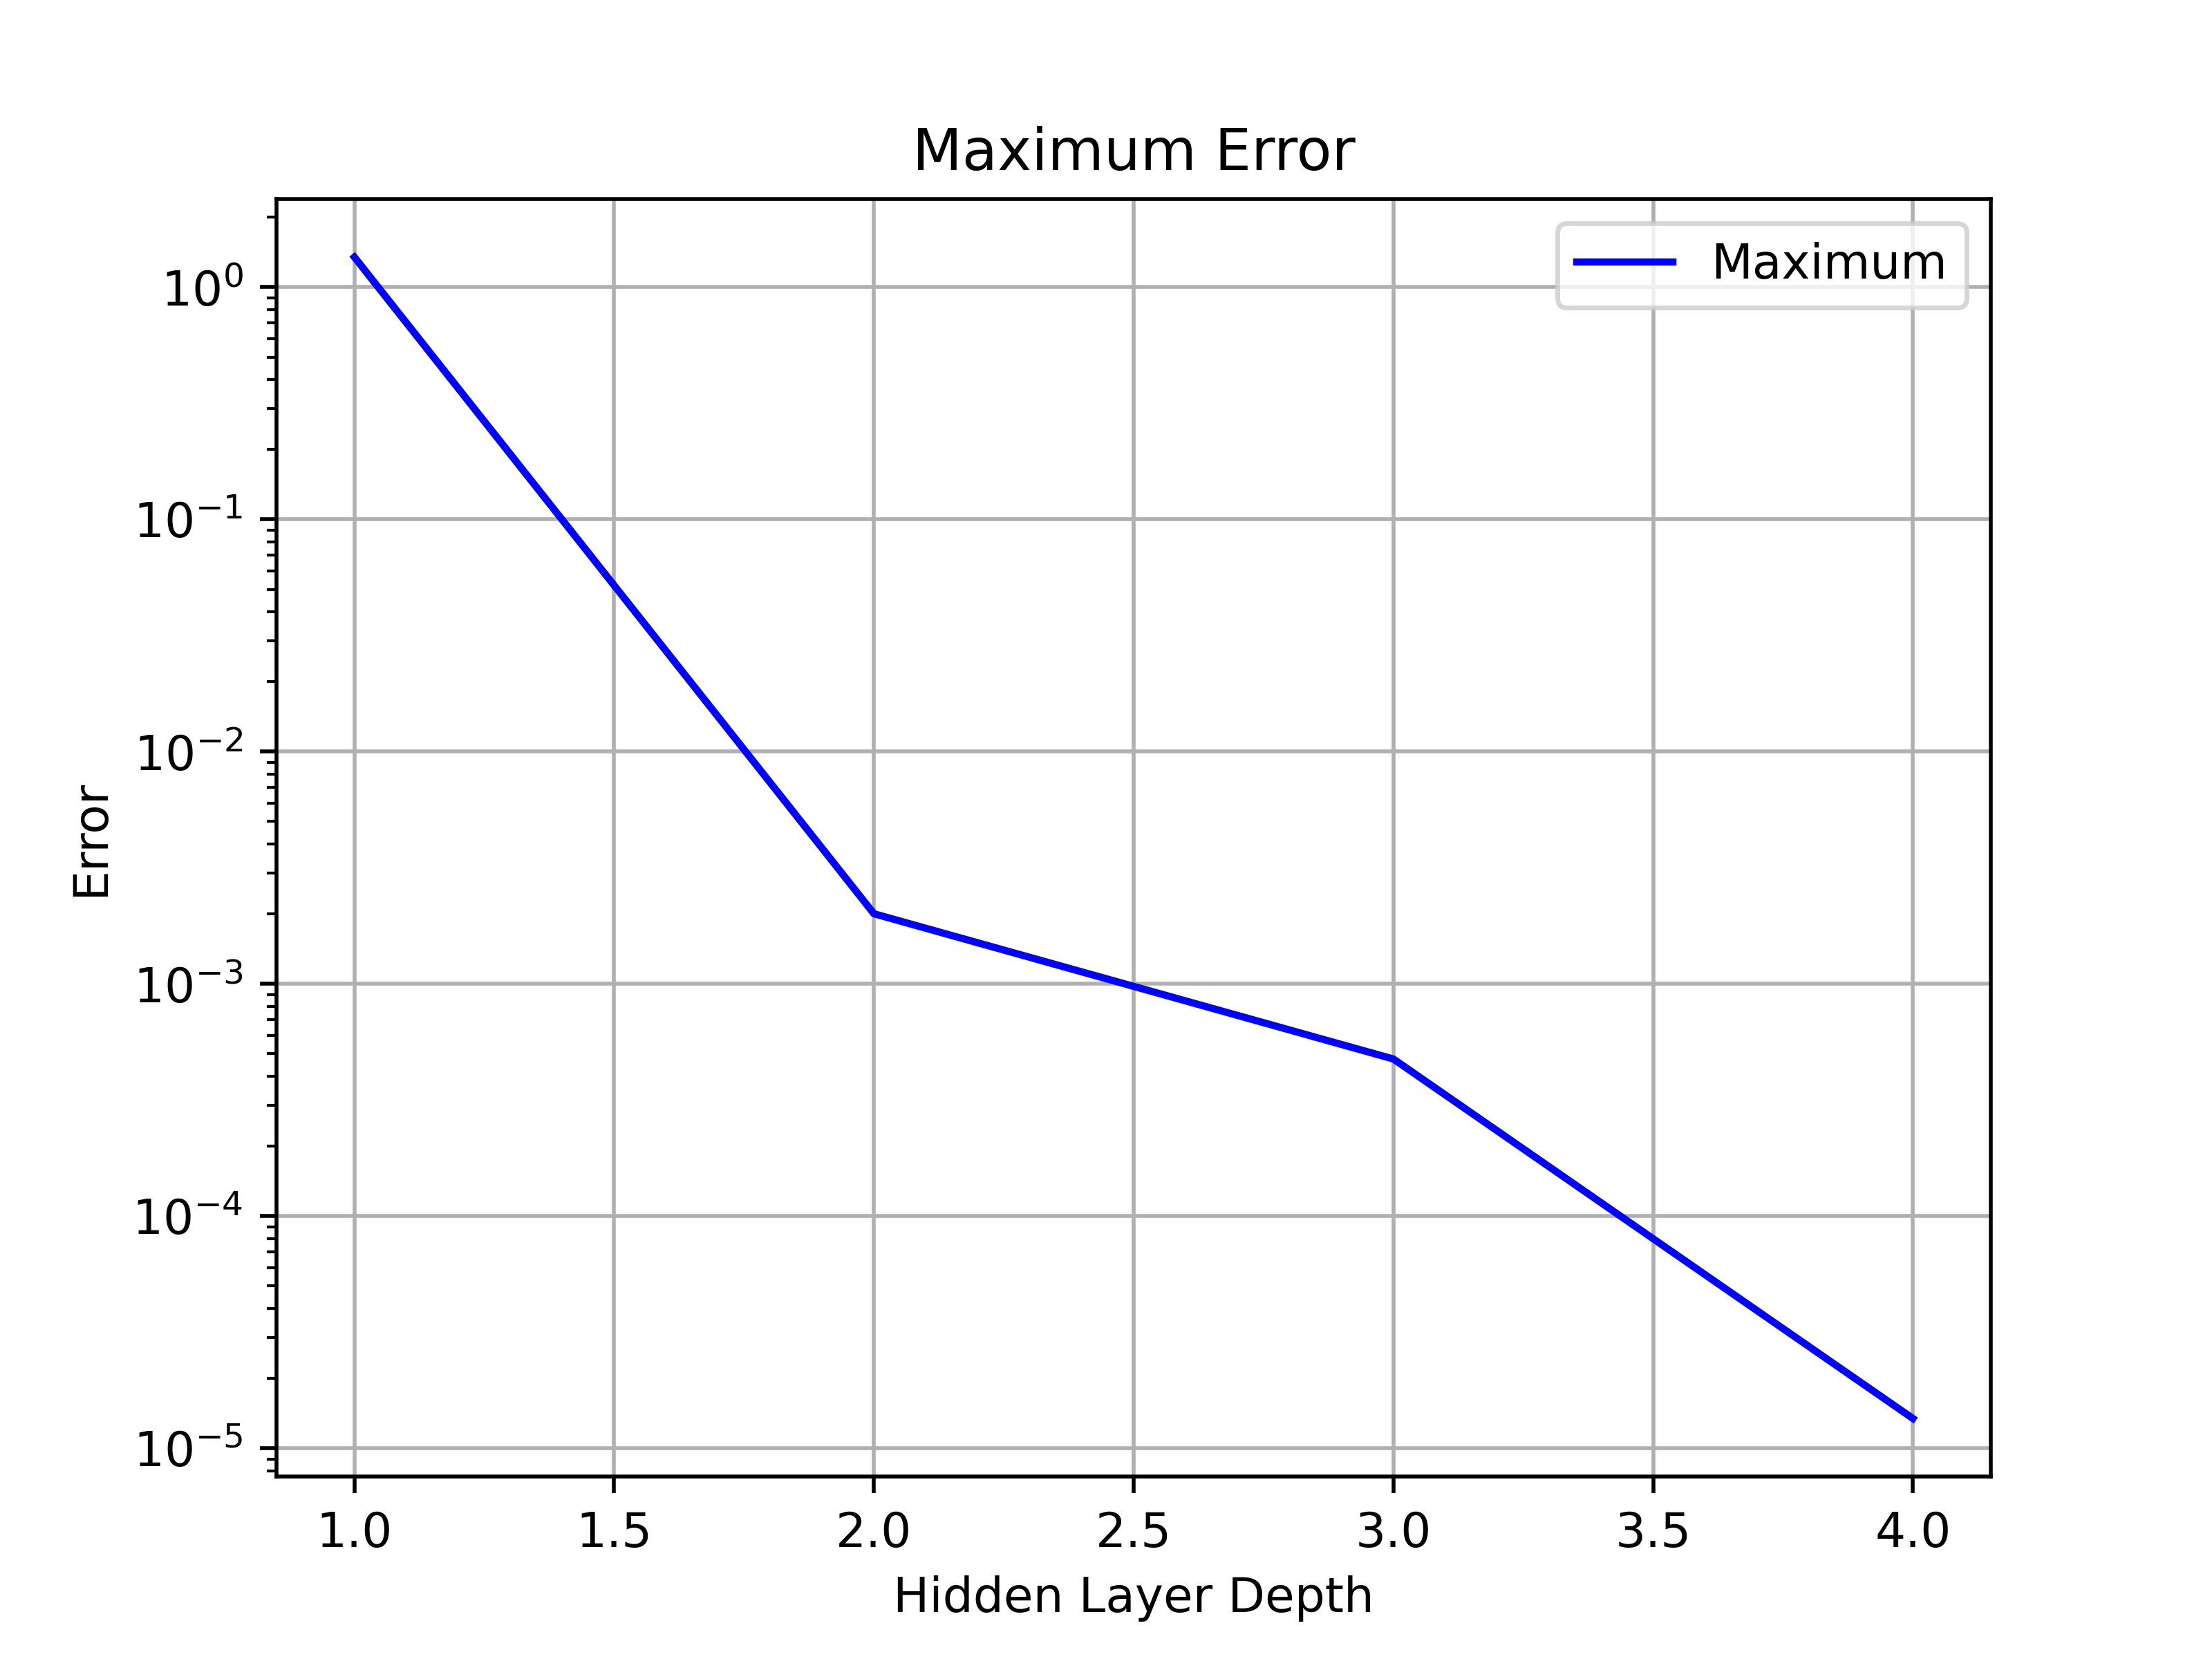
\includegraphics[scale=\size]{depthMax.png}


%Seperator
%Seperator
%Seperator
\section{Neural Network Breadth Study}
\begin{comment}
\end{comment}
The same procedure is performed as the previous section but this time the nodes on each hidden layers is varied. The depth of the hidden layers used is fixed at $4$ and the activation function for all of the hidden layers is set to hyperbolic tangent. For hidden layers of depth $4$ and $100$ nodes at each hidden layer,
\\~\\For hidden layers of depth $4$ and $80$ nodes at each hidden layer,
\\~\\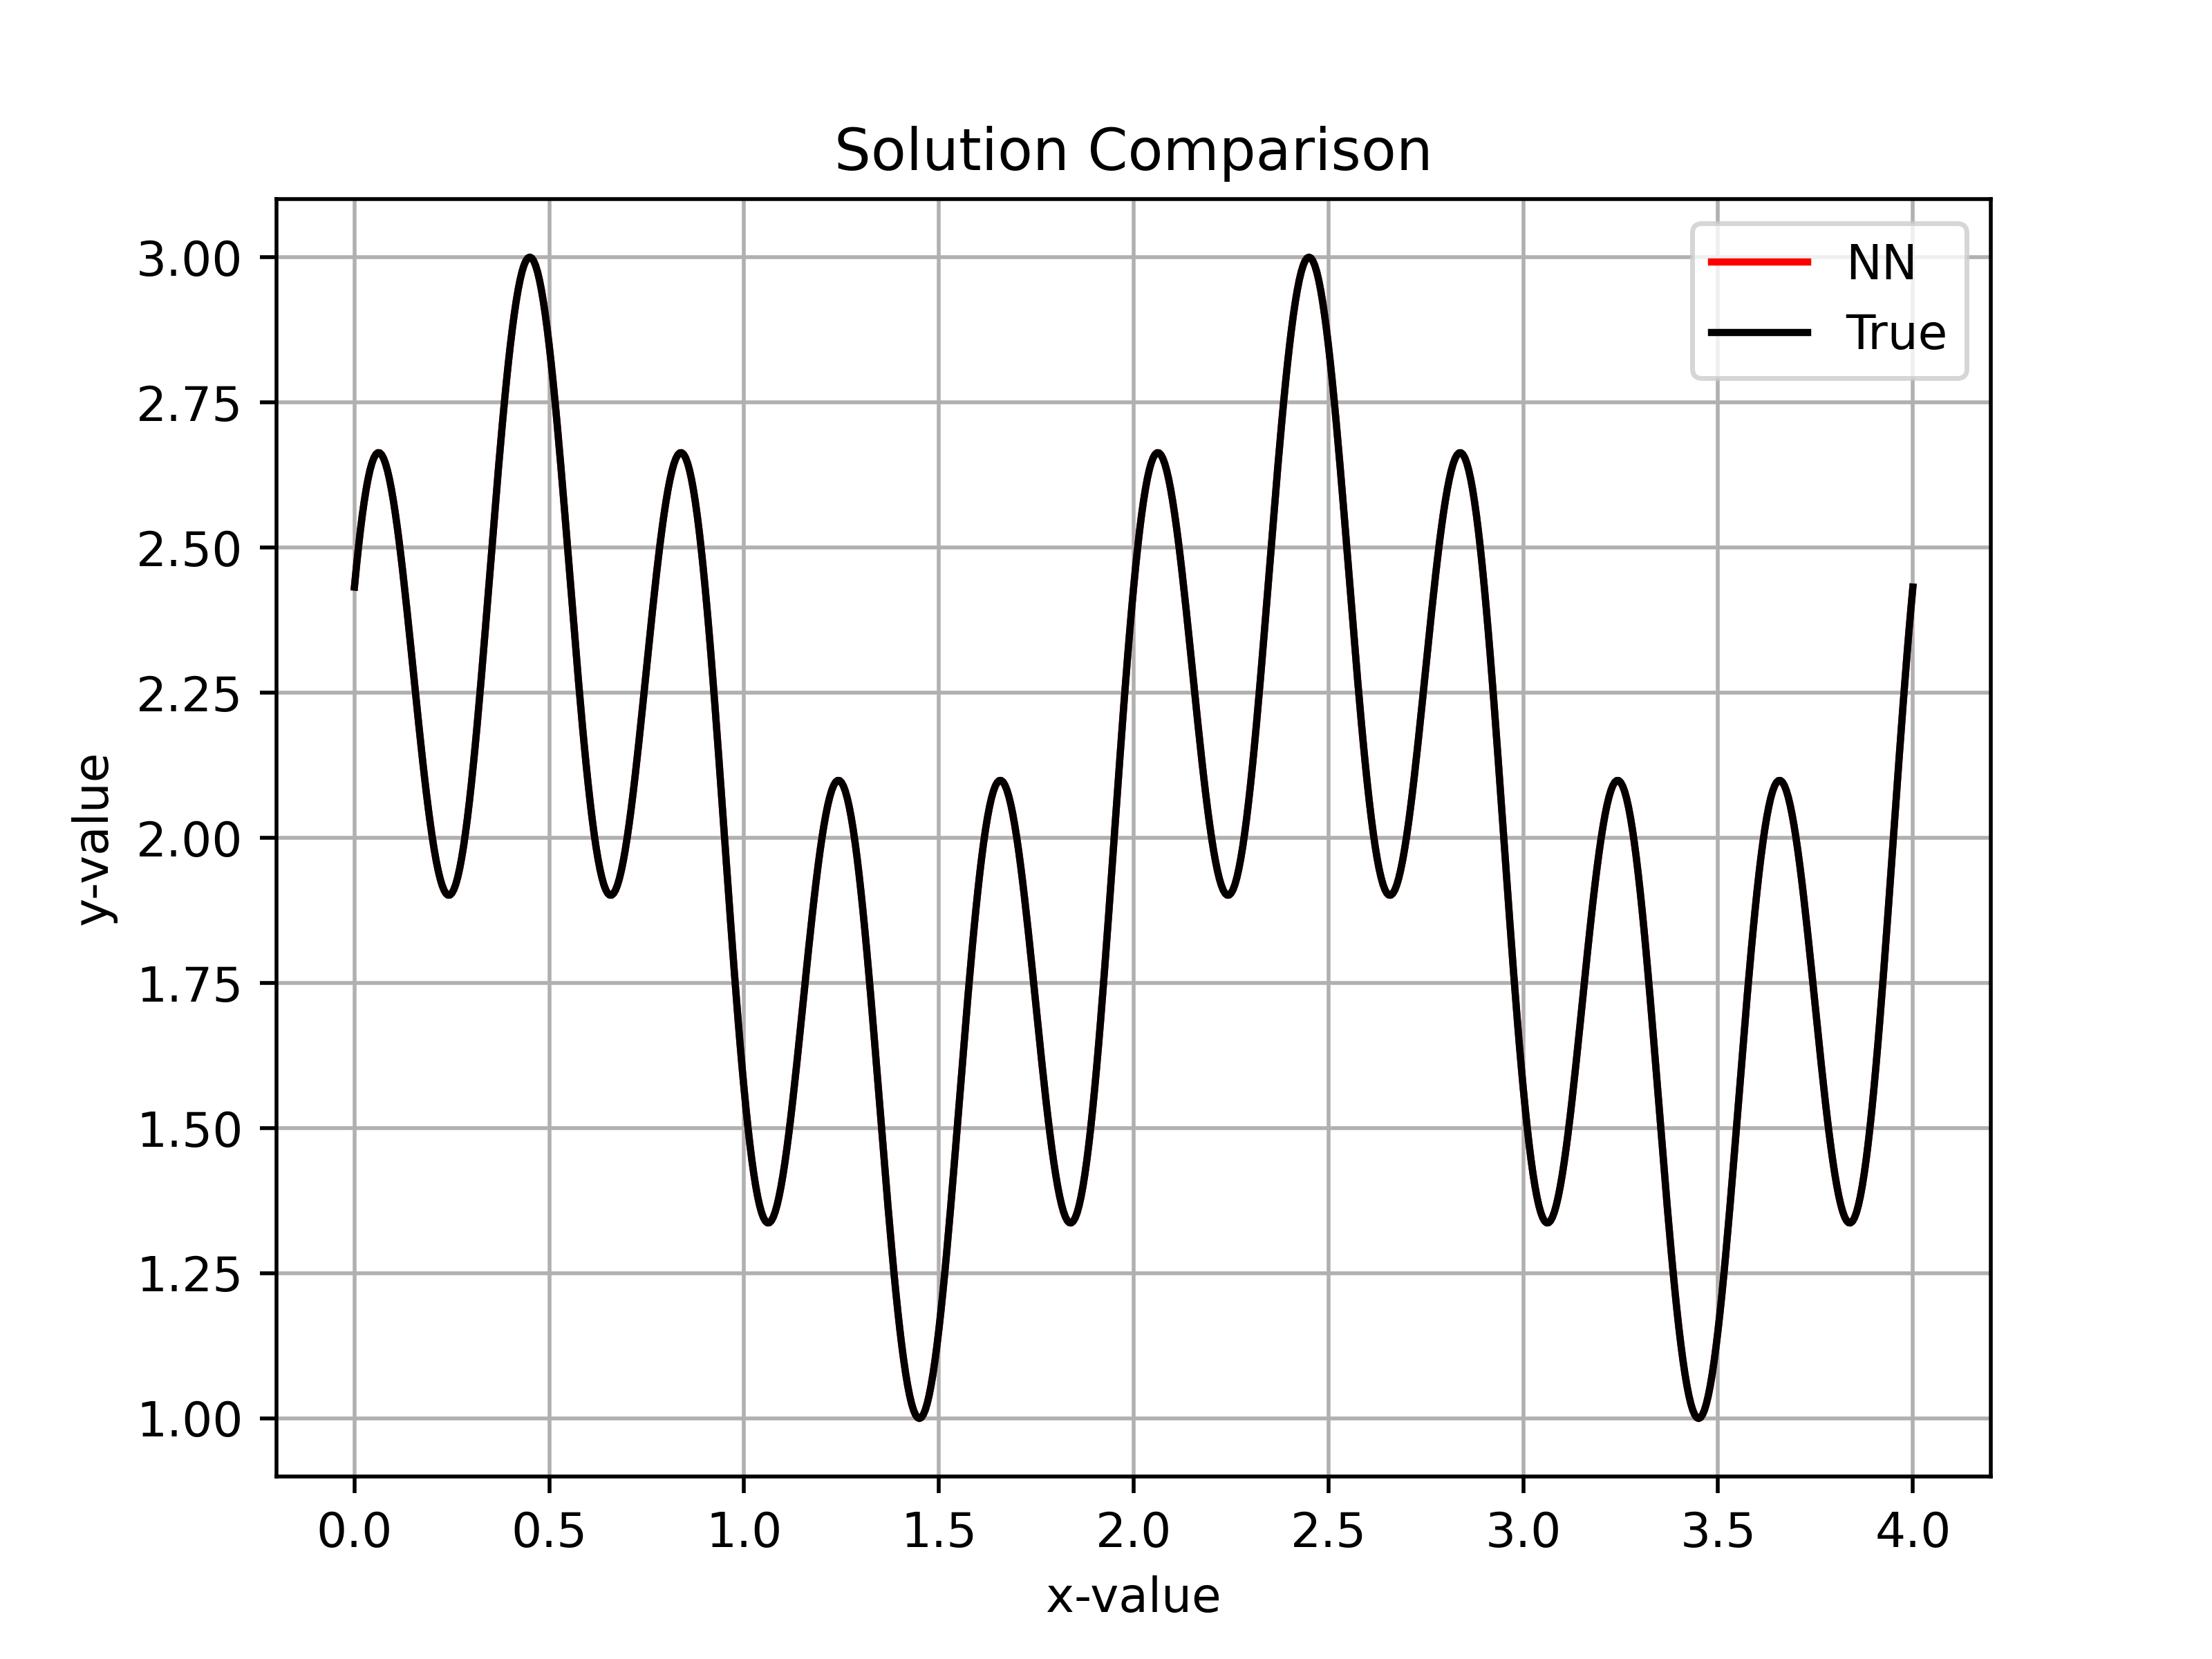
\includegraphics[scale=\size]{breadthsol80.png}
\\~\\The corresponding error along the length of the domain,
\\~\\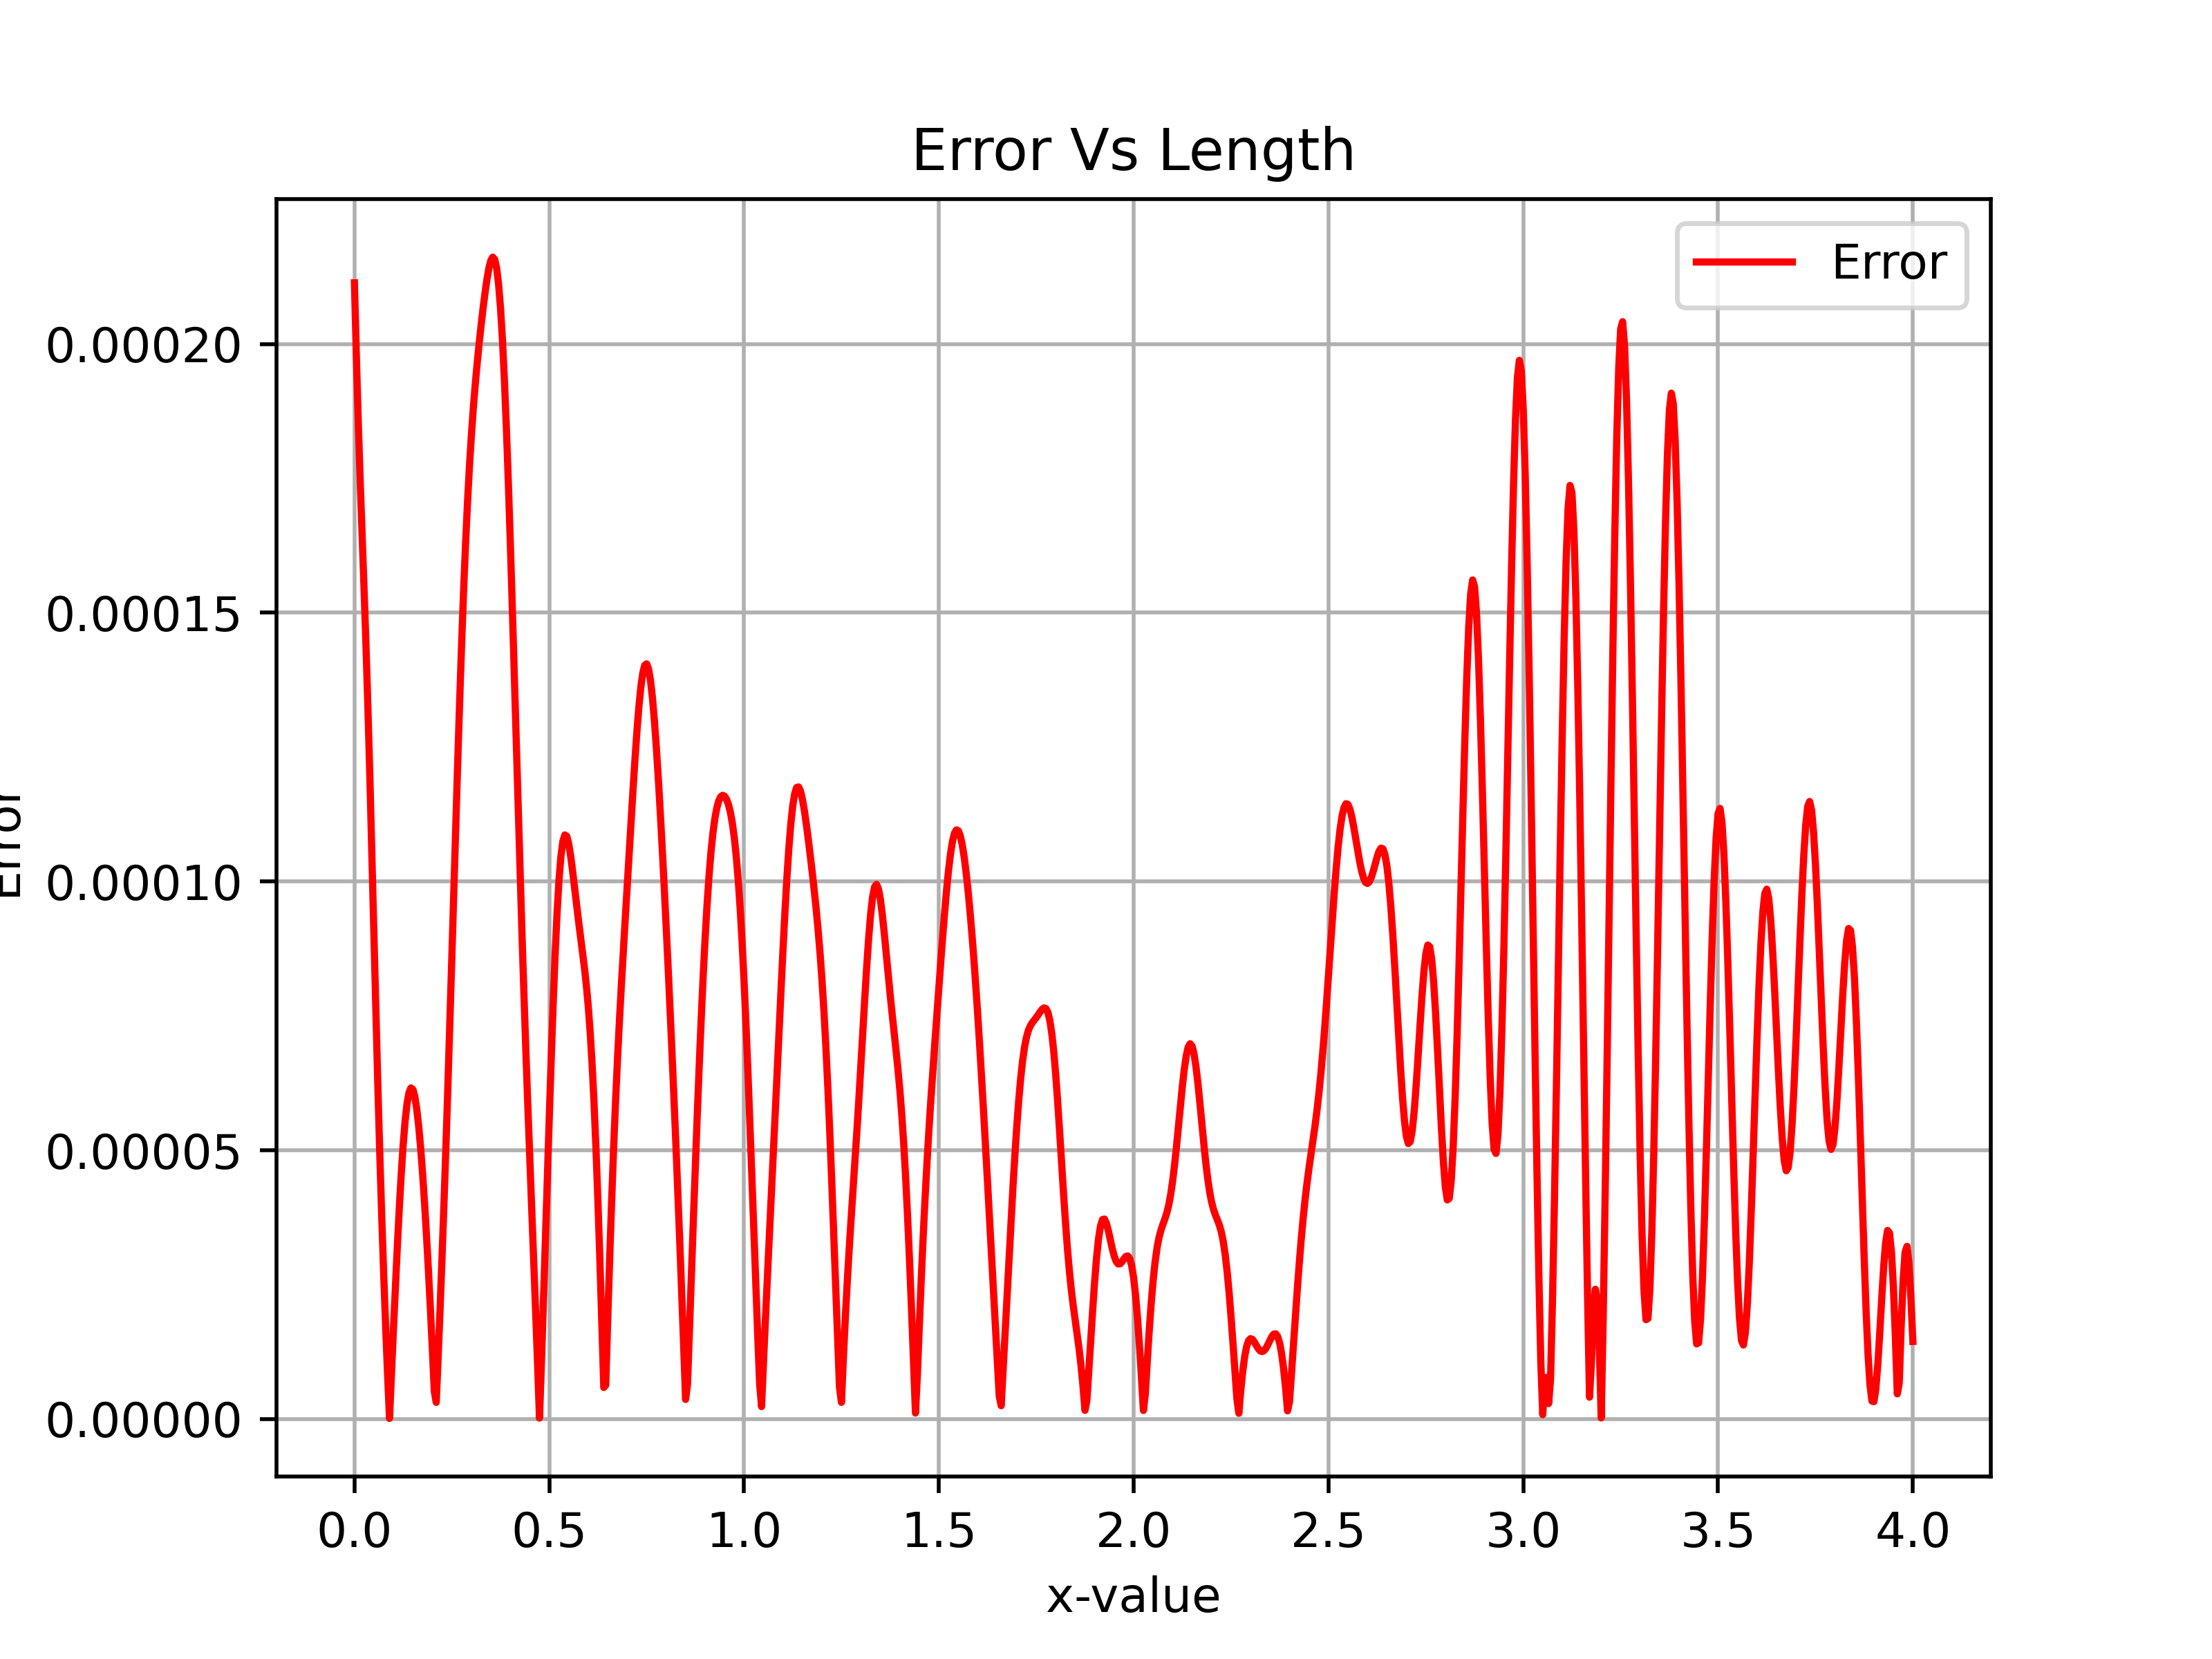
\includegraphics[scale=\size]{breadtherr80.png}
\\~\\For hidden layers of depth $4$ and $60$ nodes at each hidden layer,
\\~\\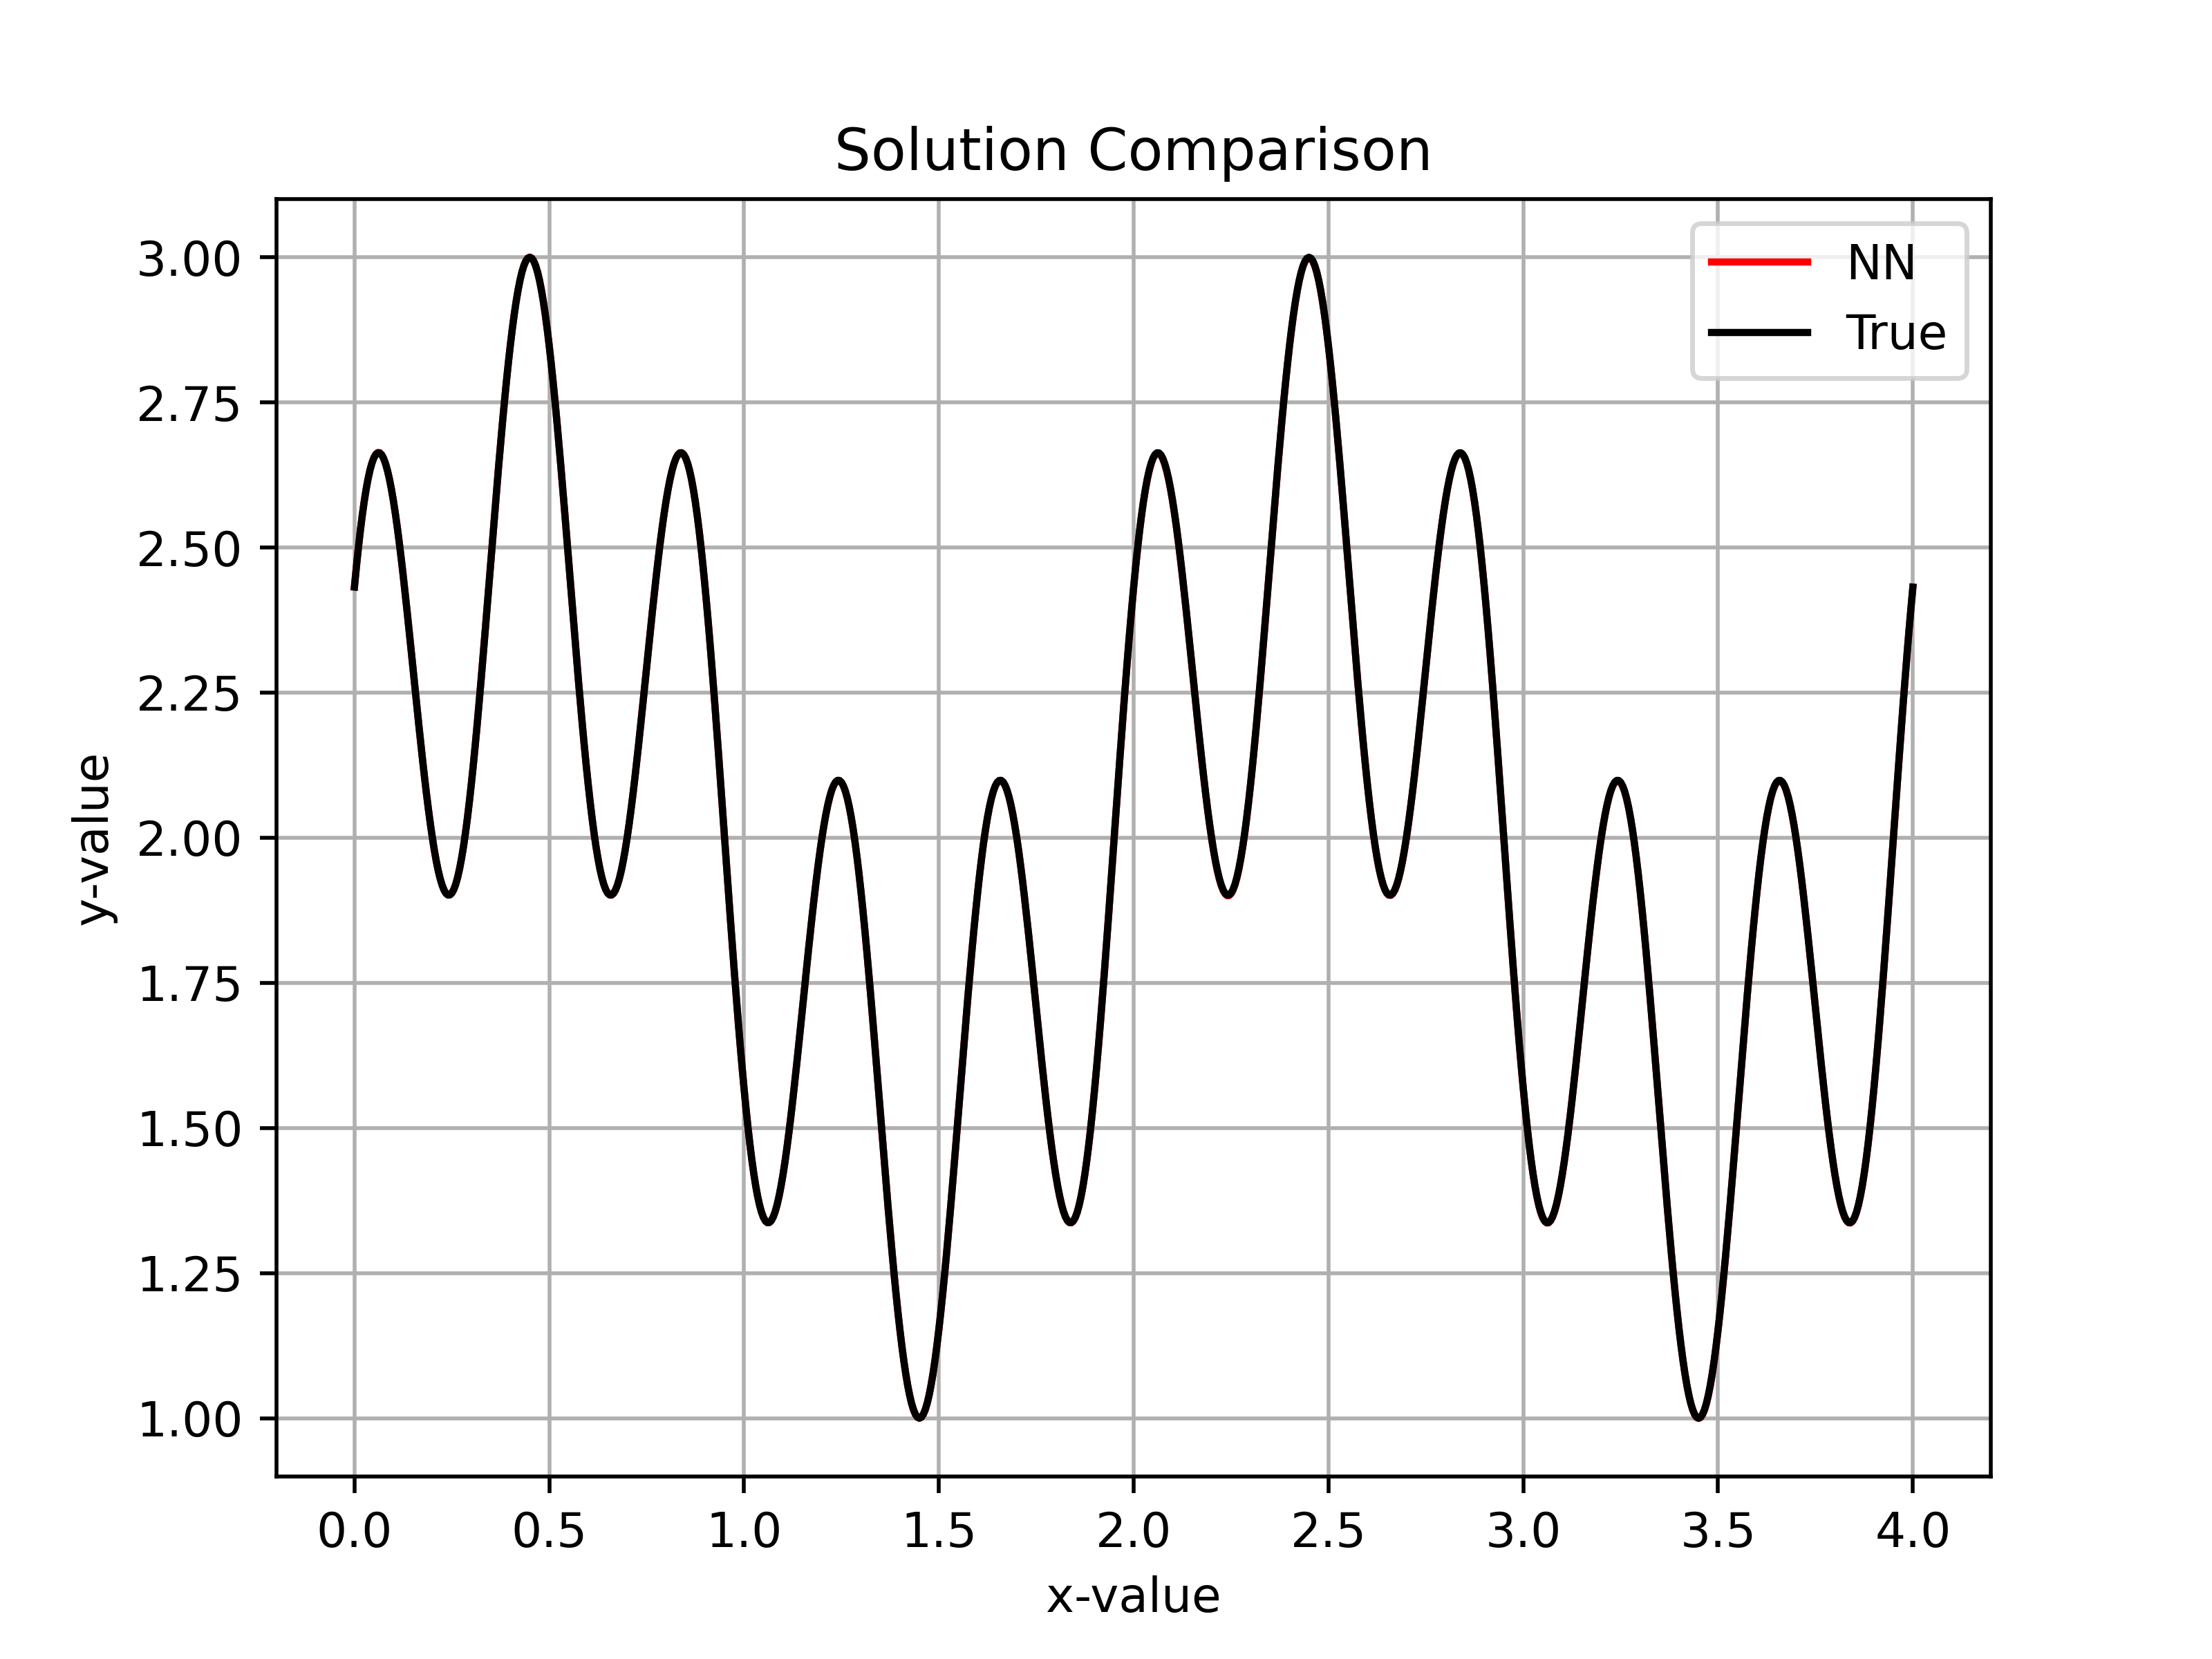
\includegraphics[scale=\size]{breadthsol60.png}
\\~\\The corresponding error along the length of the domain,
\\~\\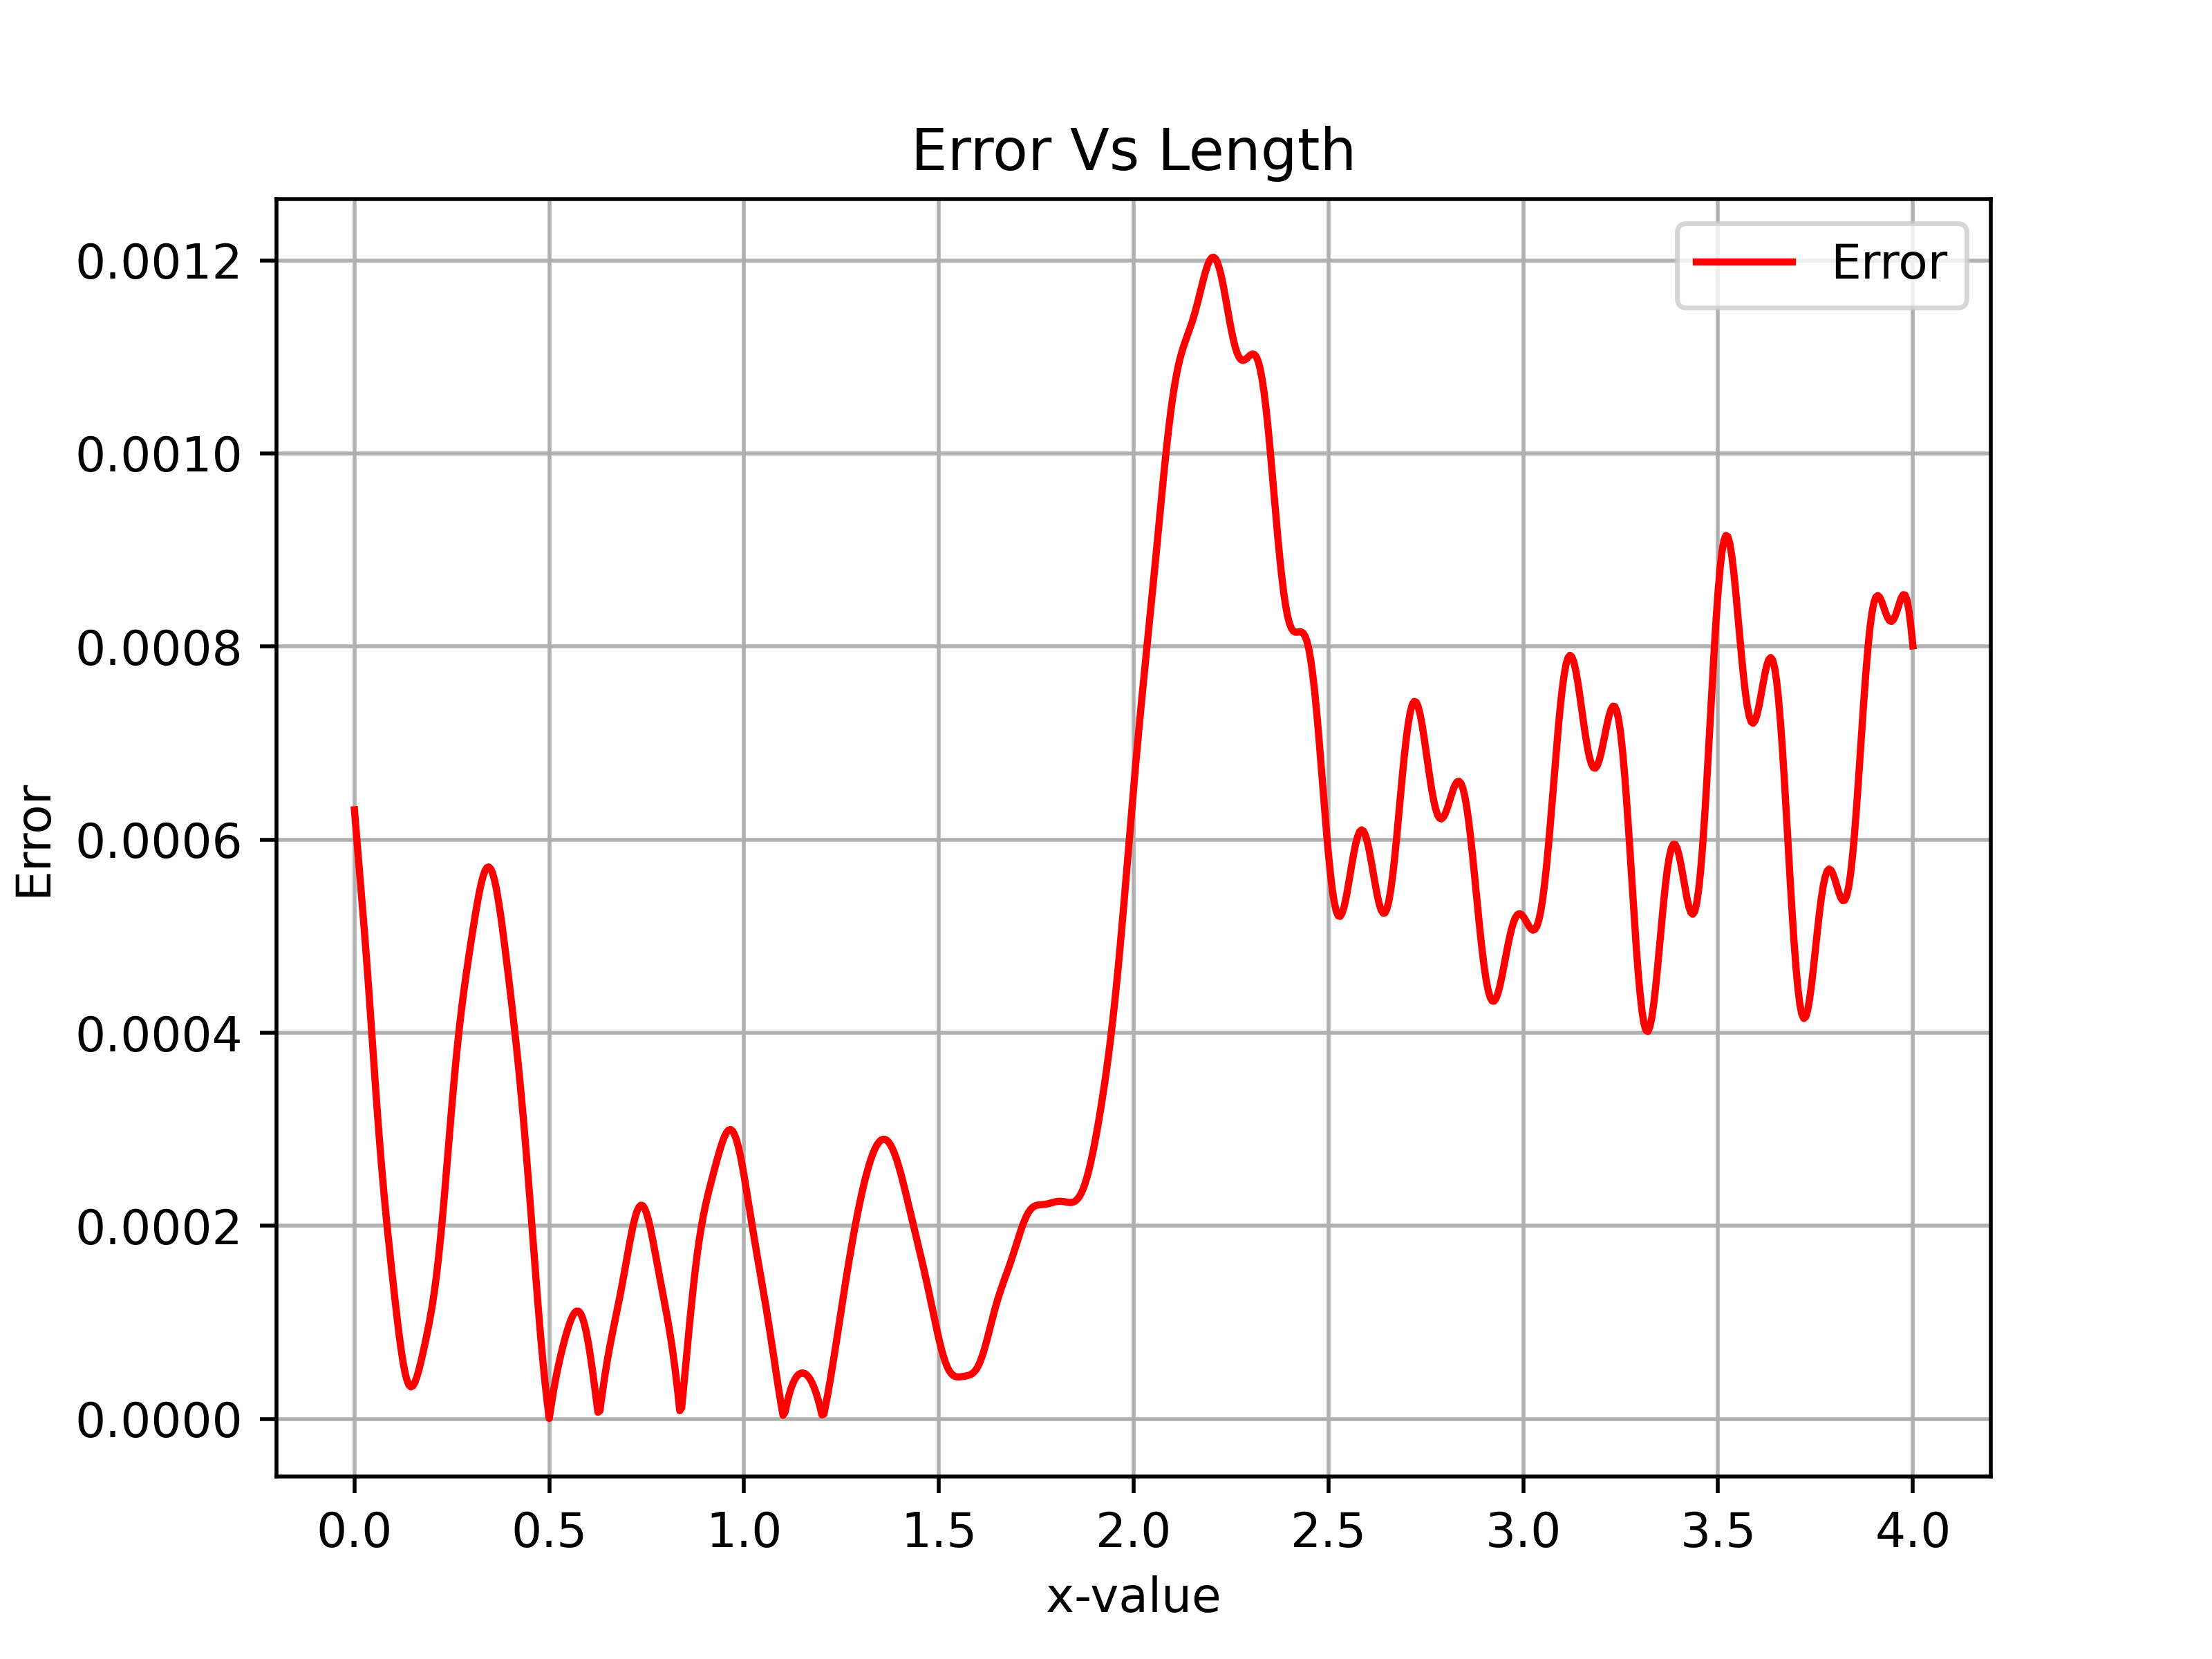
\includegraphics[scale=\size]{breadtherr60.png}
\\~\\For hidden layers of depth $4$ and $40$ nodes at each hidden layer,
\\~\\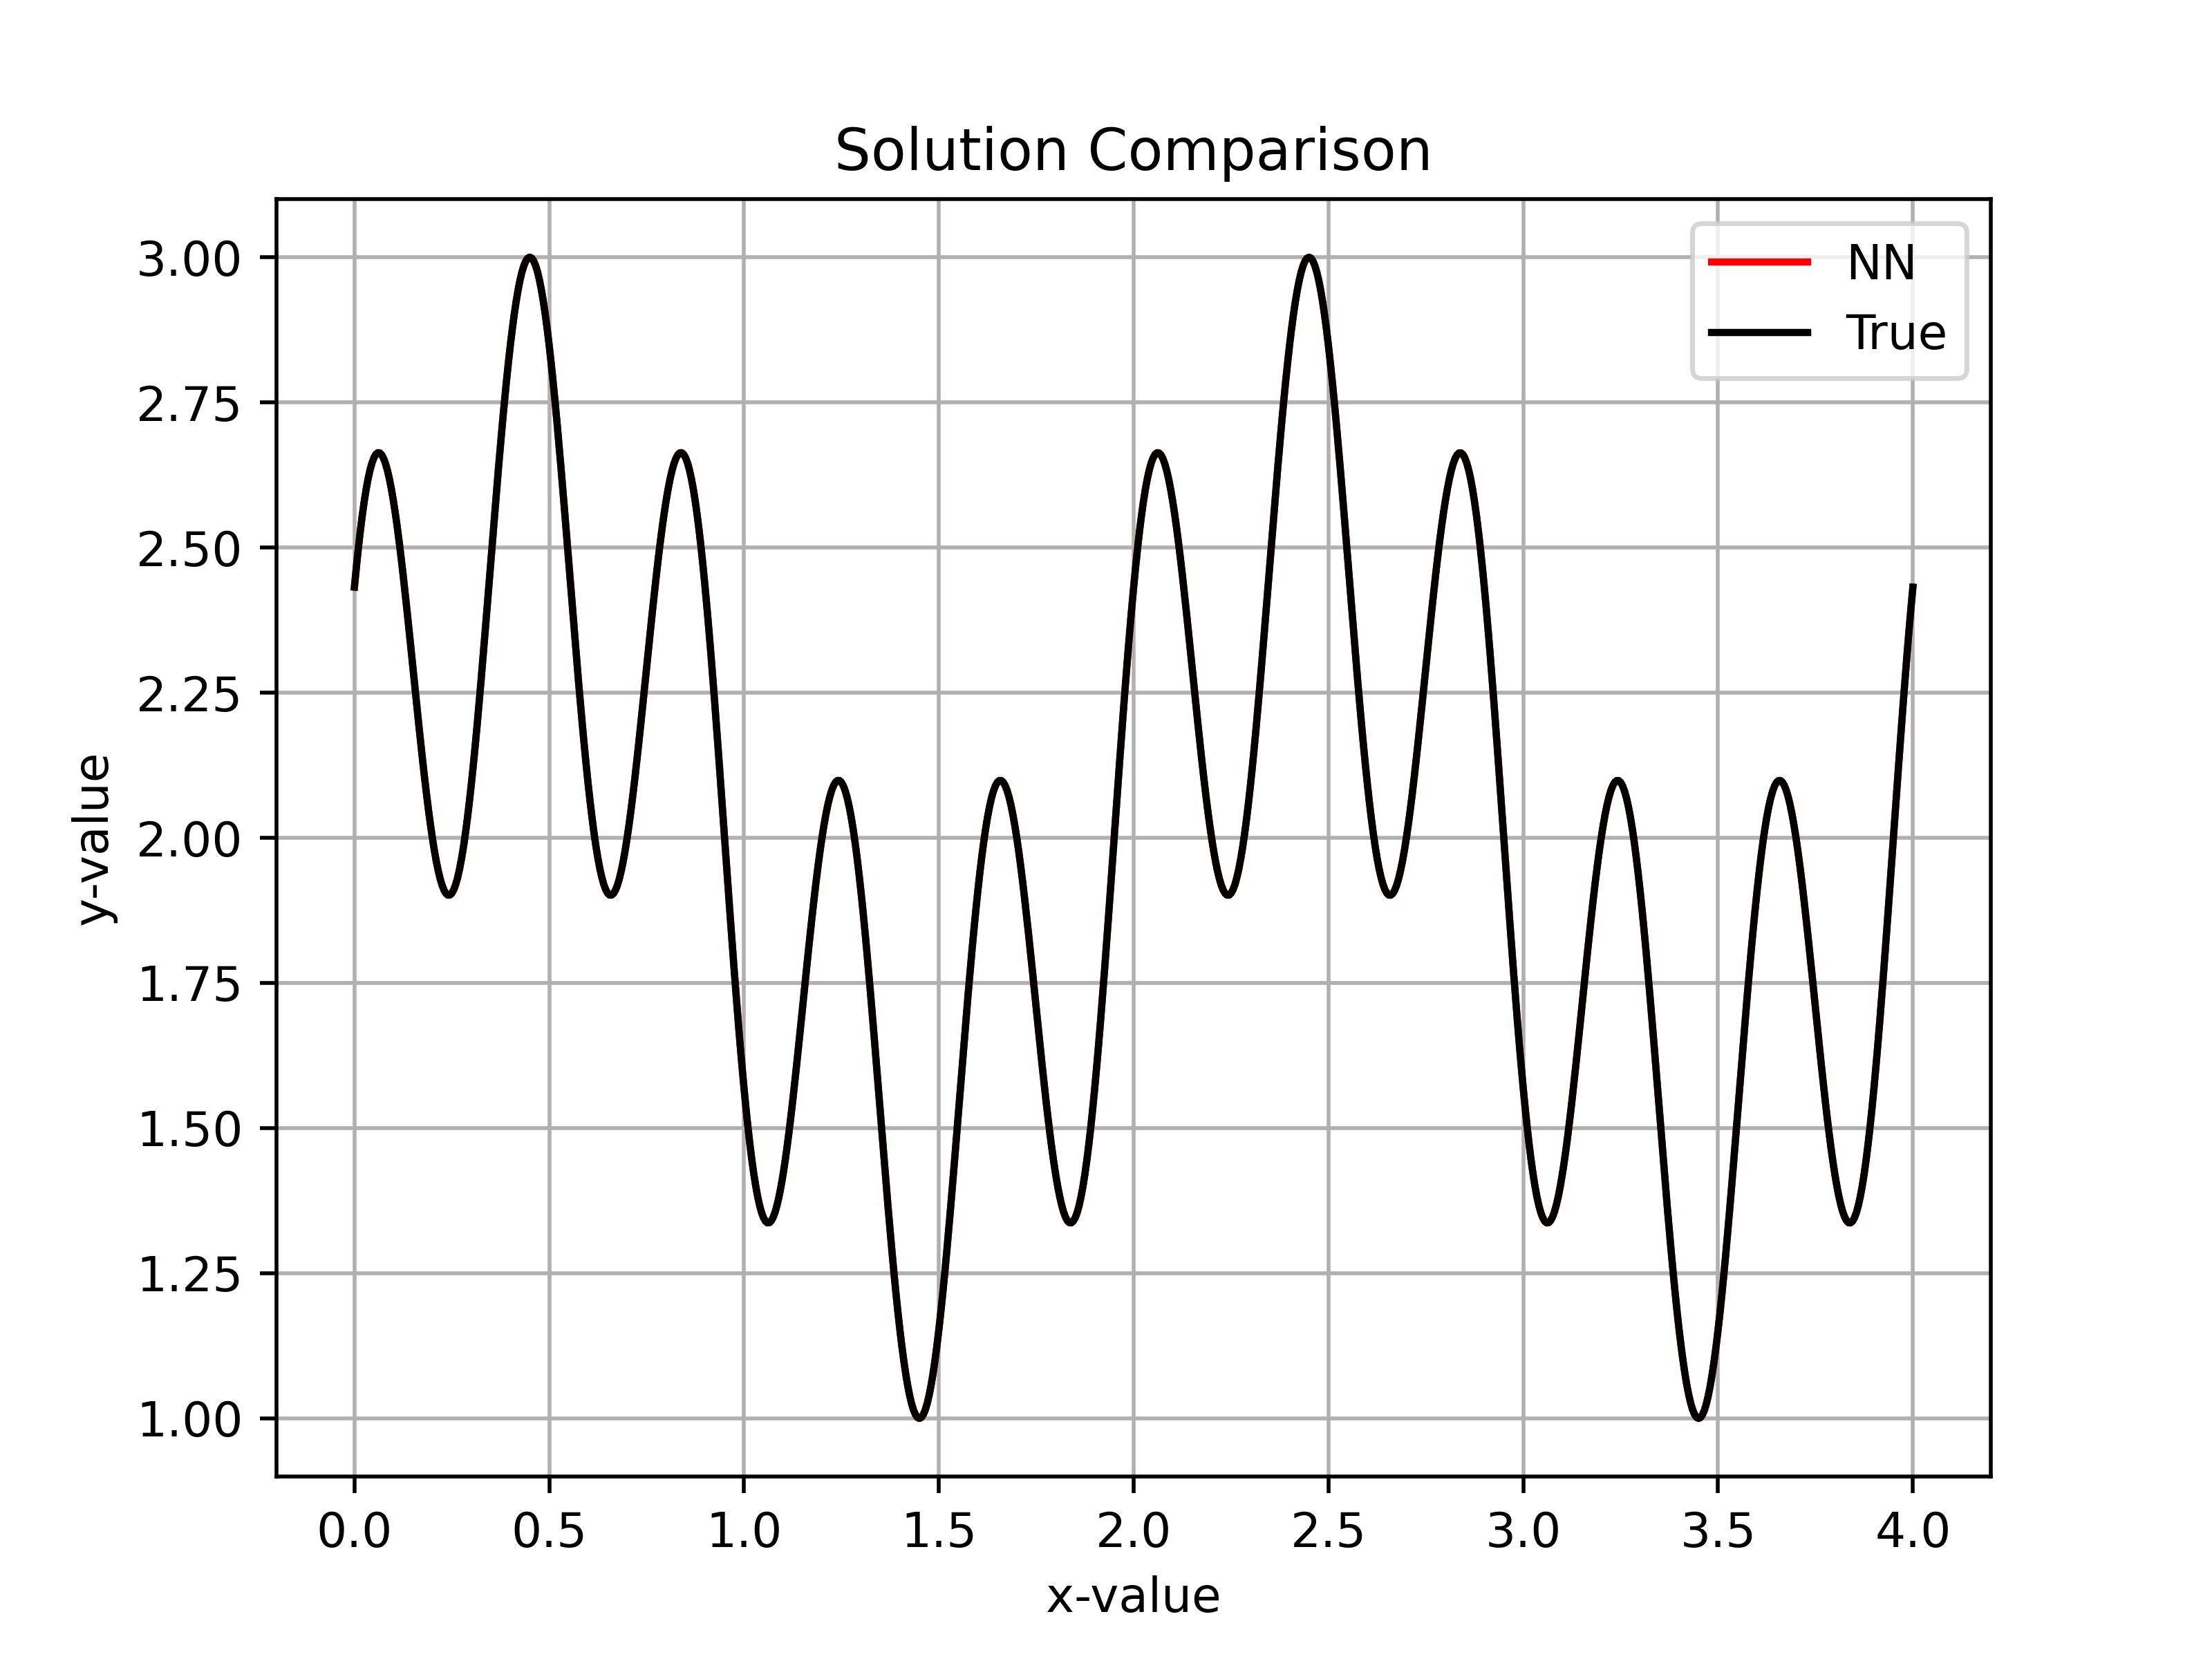
\includegraphics[scale=\size]{breadthsol40.png}
\\~\\The corresponding error along the length of the domain,
\\~\\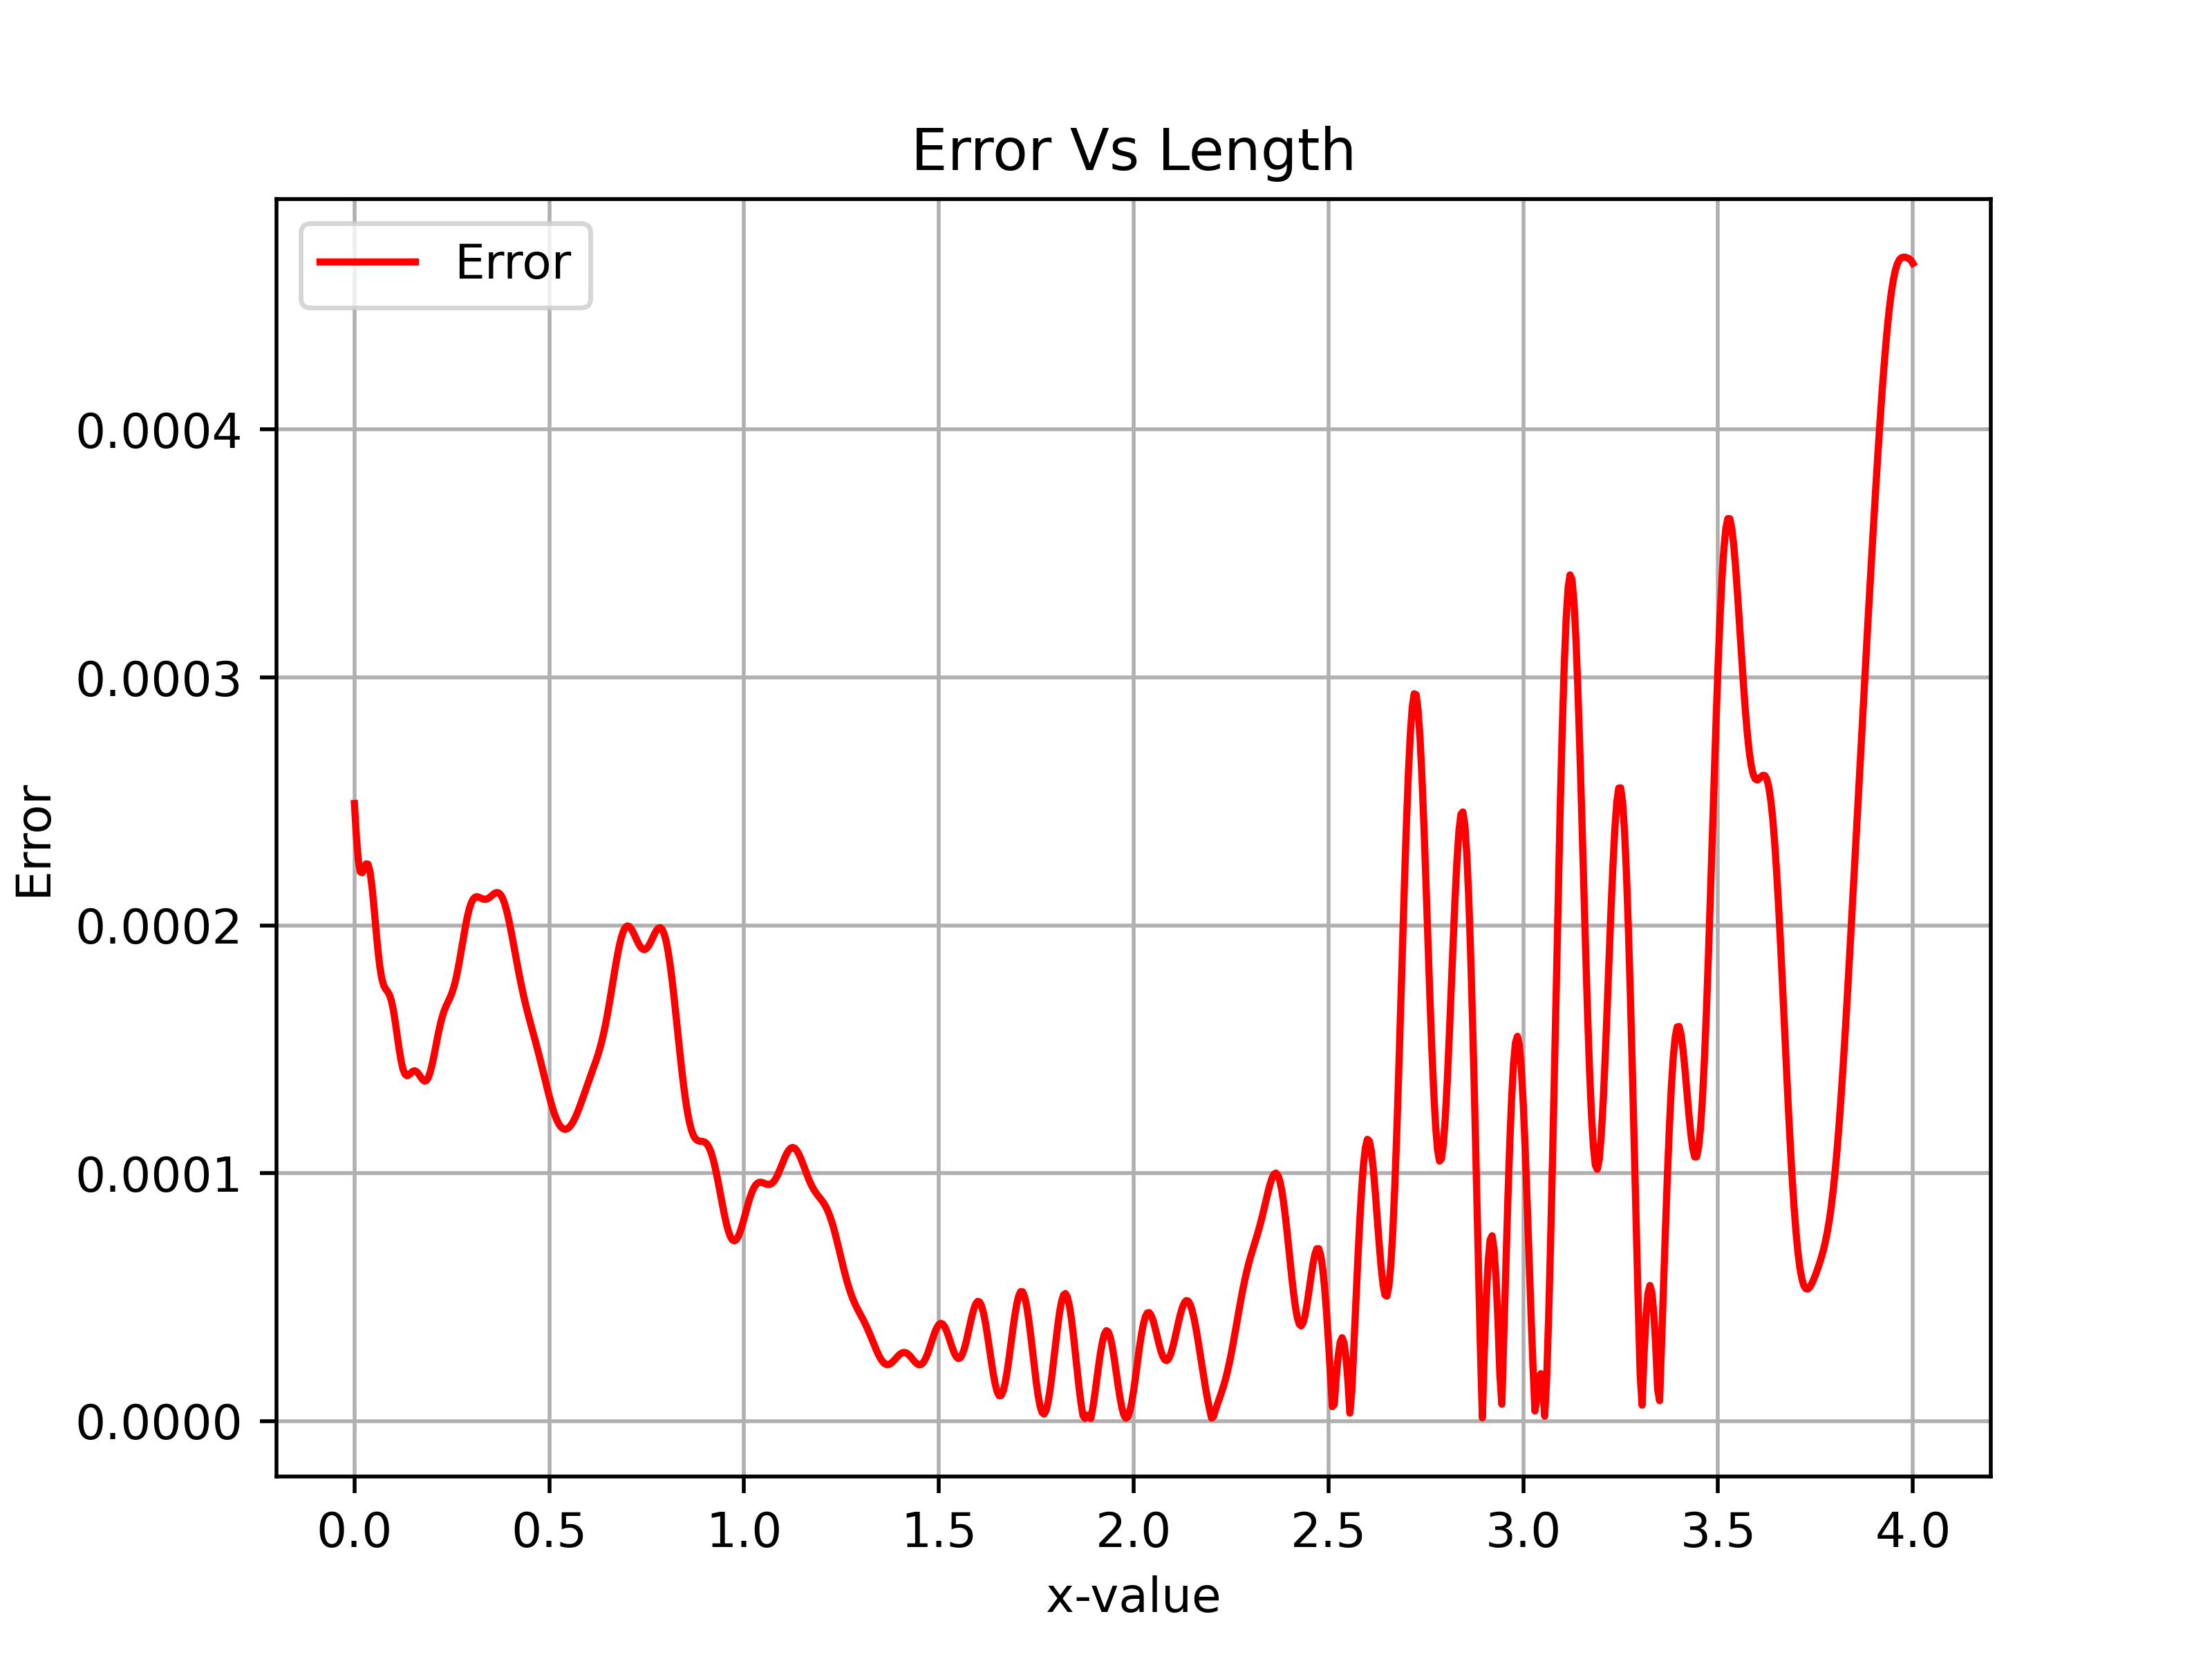
\includegraphics[scale=\size]{breadtherr40.png}
\\~\\For hidden layers of depth $4$ and $20$ nodes at each hidden layer,
\\~\\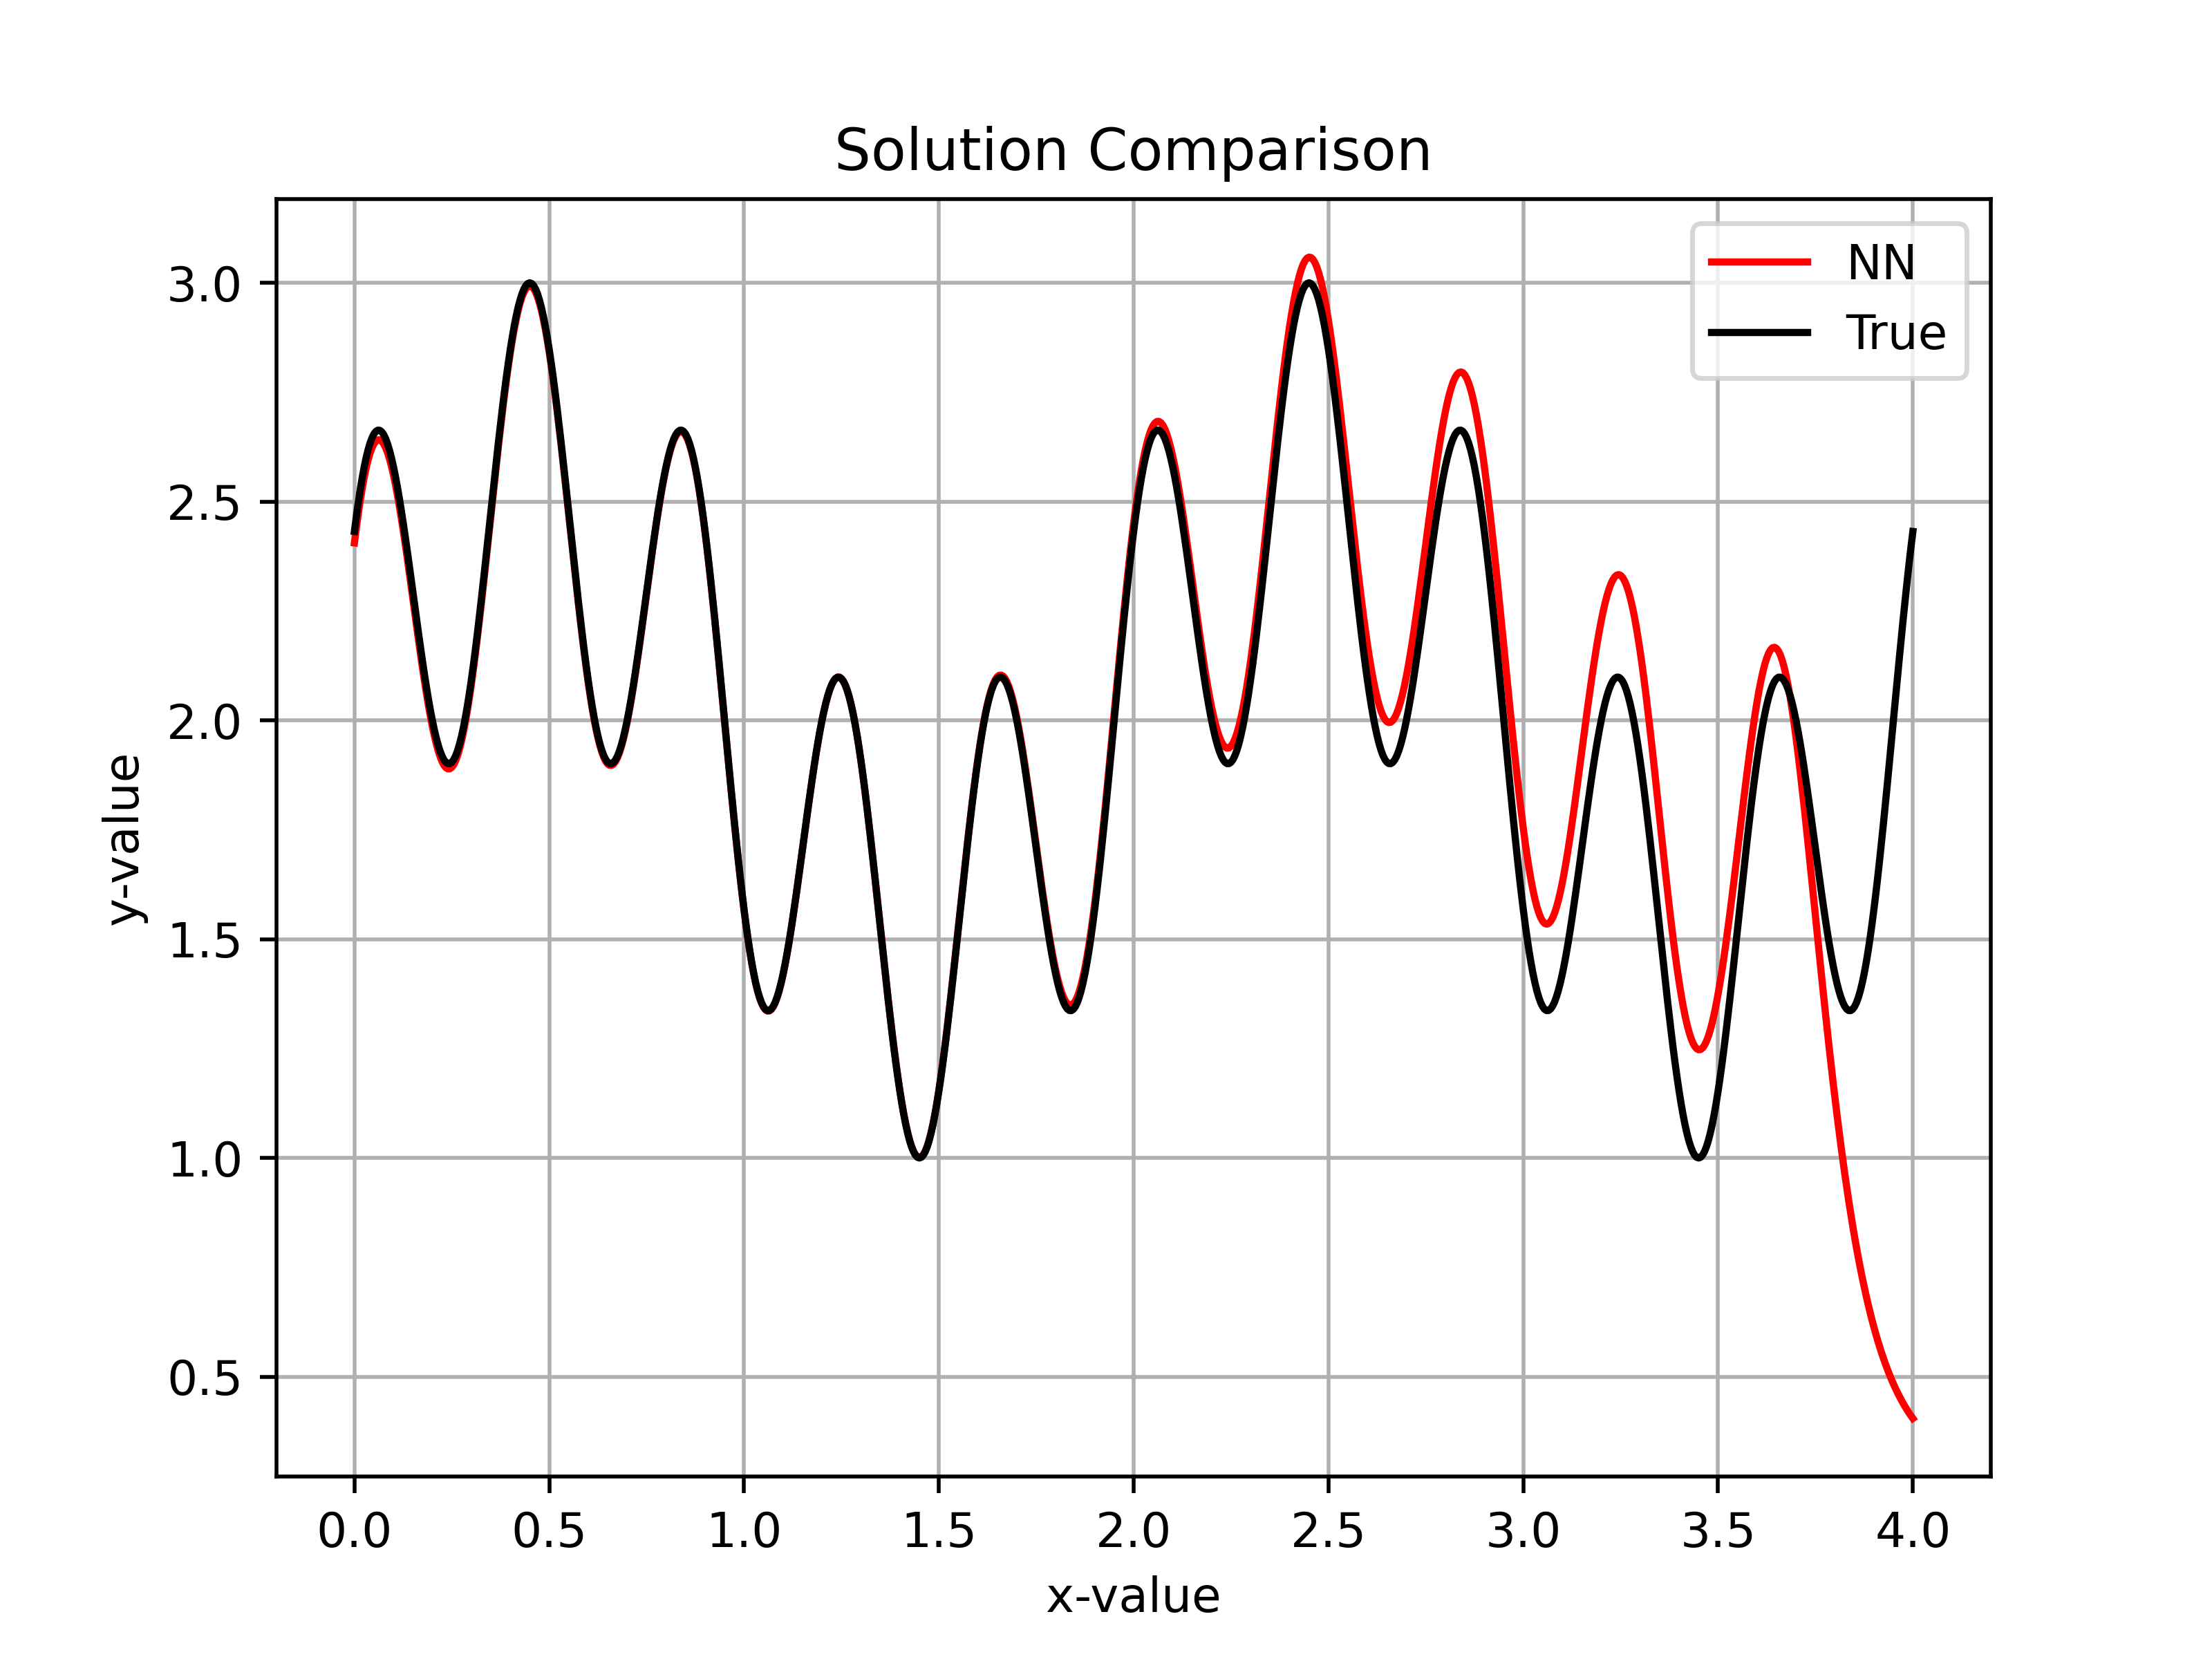
\includegraphics[scale=\size]{breadthsol20.png}
\\~\\The corresponding error along the length of the domain,
\\~\\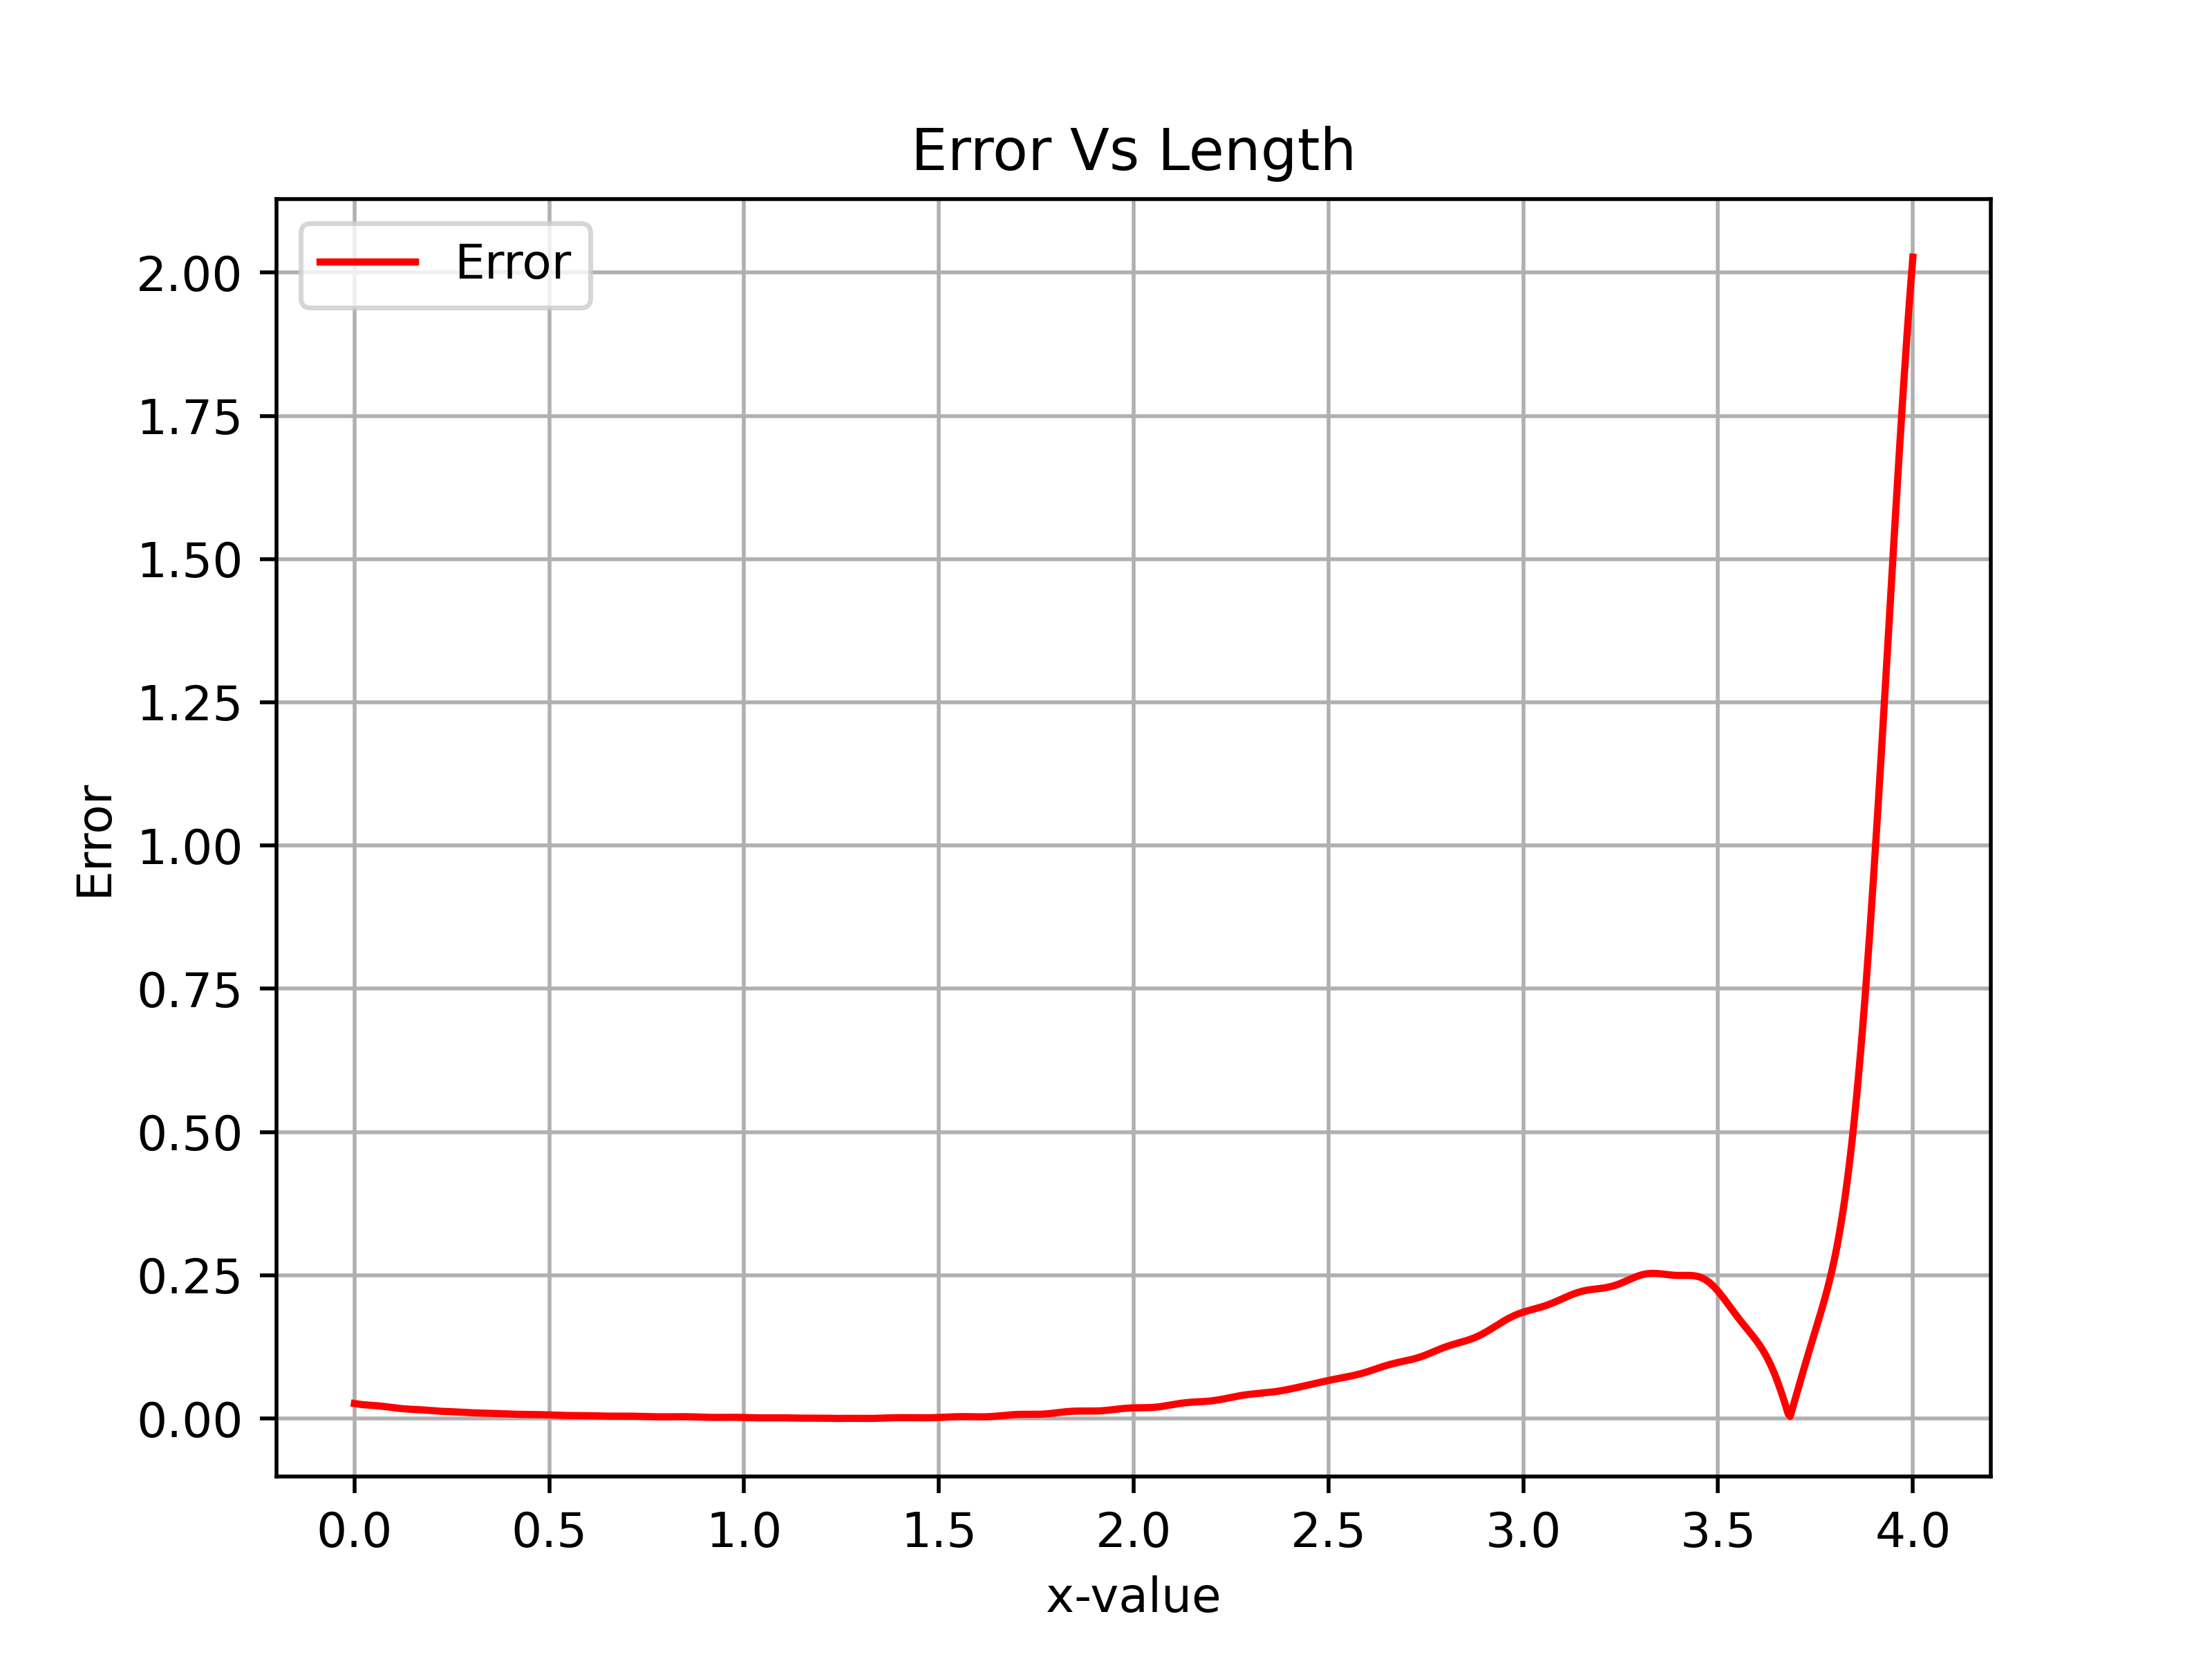
\includegraphics[scale=\size]{breadtherr20.png}
\\~\\~\\The maximum error along the entire domain is collected and plotted against the corresponding breadth of the hidden layers and is shown below,
\\~\\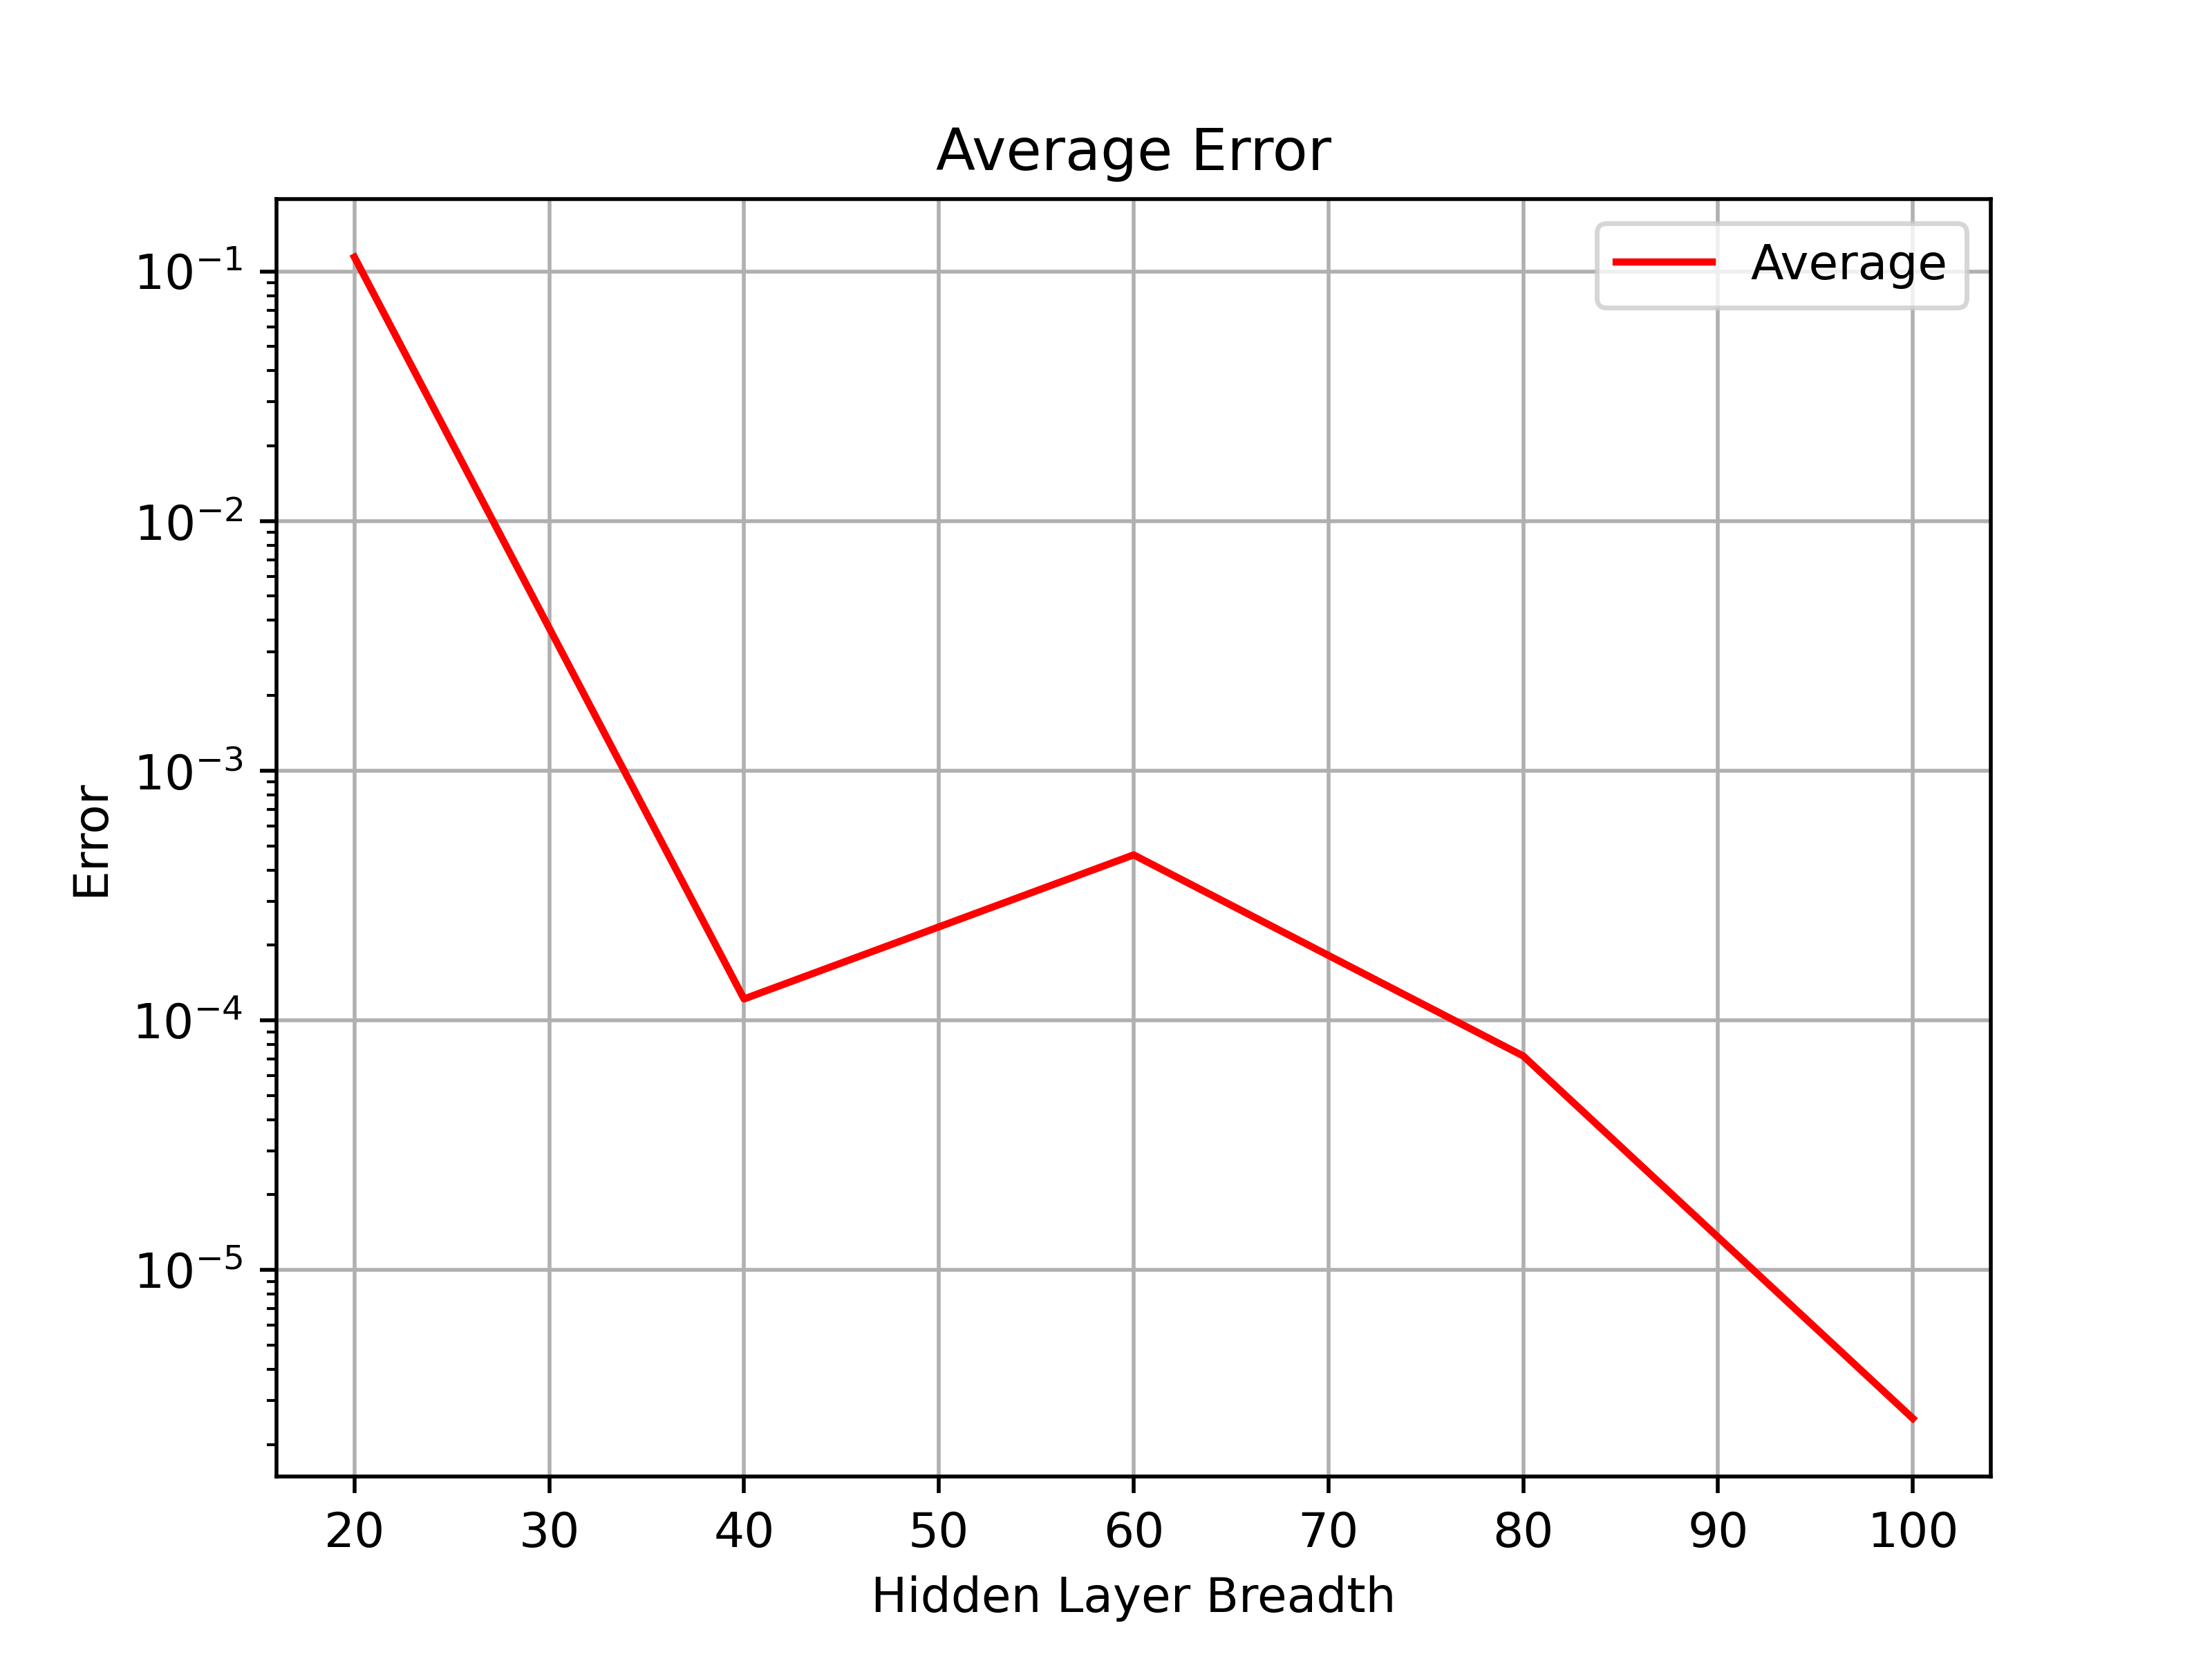
\includegraphics[scale=\size]{breadthMean.png}
\\~\\The average error along the entire domain is shown below,
\\~\\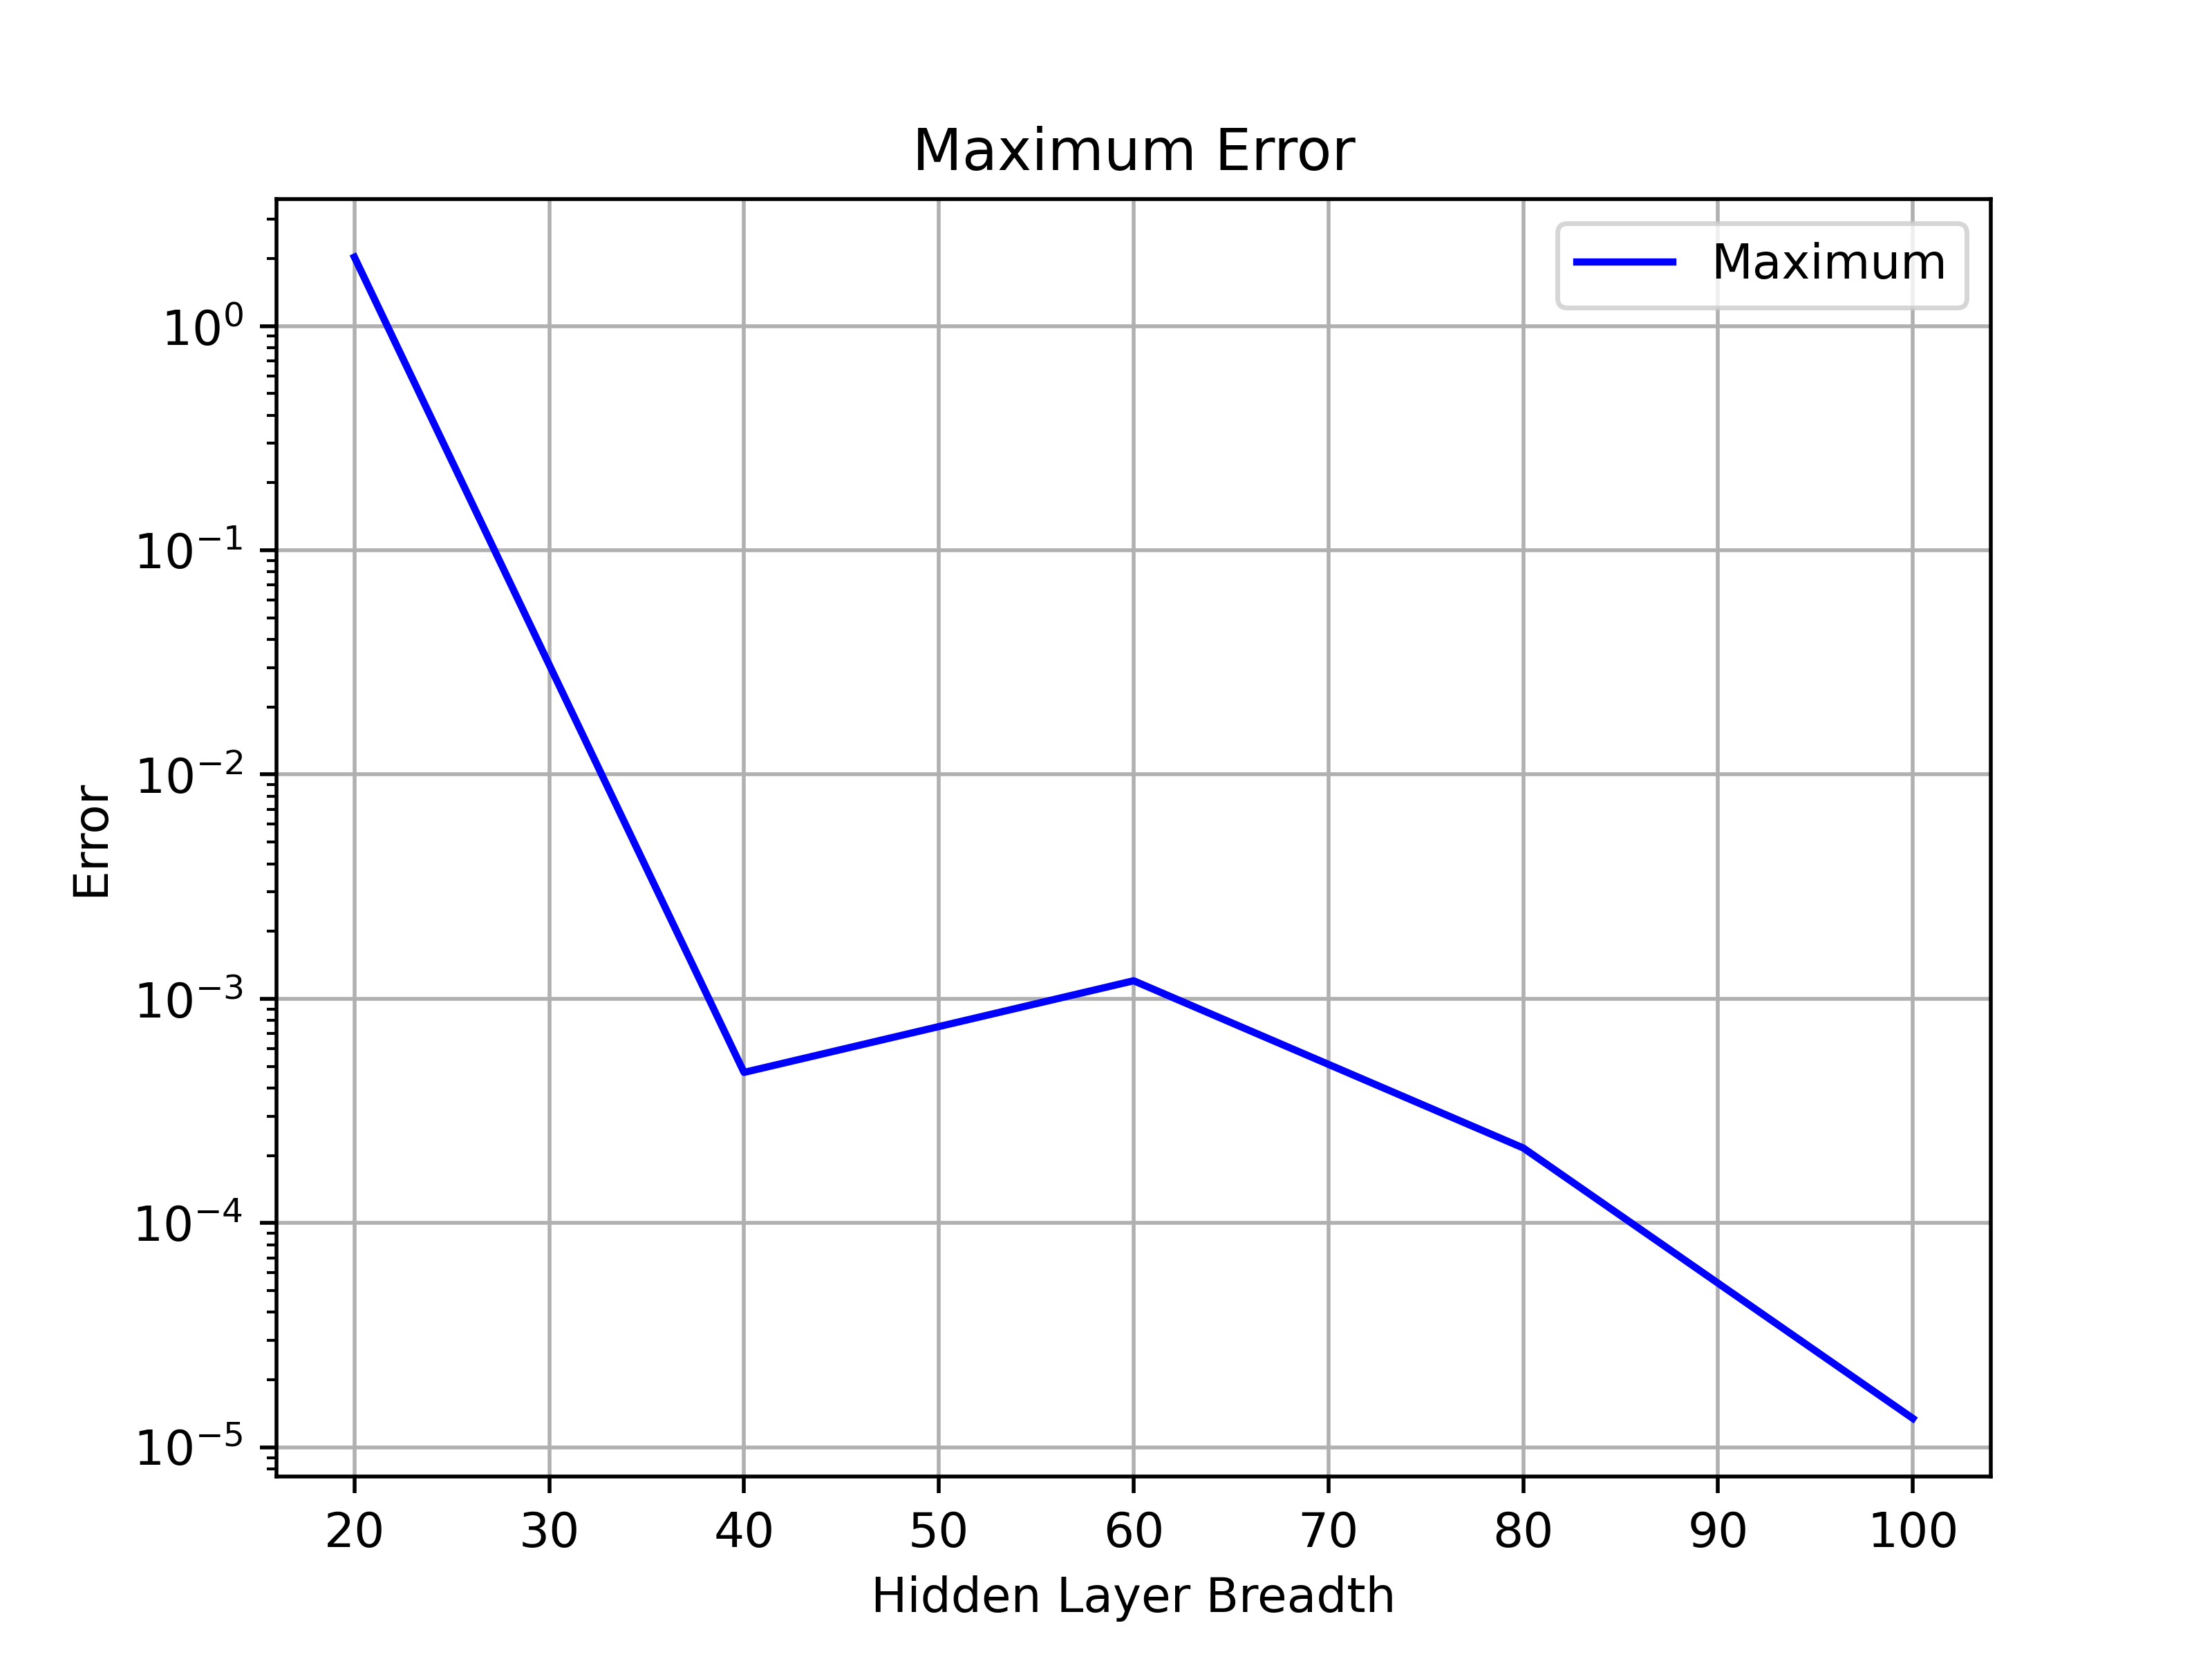
\includegraphics[scale=\size]{breadthMax.png}
%Seperator
%Seperator
%Seperator
\section{Appendix}
\begin{comment}
\end{comment}
The python script that was used to generate the solution plots is shown below,
\begin{lstlisting}[language=python]
#Author: Hans C. Suganda
import matplotlib.pyplot as plt
import numpy as np

#Reading from Files
data = np.genfromtxt("breadth20.dat")

#Parsing the titles
data = data[1::,:]

#Error
aveError = np.mean(data[:,3])
maxError = max(data[:,3])
print(maxError, aveError)

#Plotting Solutions Plot
plt.figure(1)
plt.plot(data[:,0], data[:,1], '-r', label='NN')
plt.plot(data[:,0], data[:,2], '-k', label='True')
plt.xlabel('x-value')
plt.ylabel('y-value')
plt.title('Solution Comparison')
plt.legend()
plt.grid()
plt.savefig('breadthsol20.png', dpi=500)

#Plotting Error
plt.figure(2)
plt.plot(data[:,0], data[:,3], '-r', label='Error')
plt.xlabel('x-value')
plt.ylabel('Error')
plt.title('Error Vs Length')
plt.legend()
plt.grid()
plt.savefig('breadtherr20.png', dpi=500)

plt.show()
\end{lstlisting}
$$$$
The python script that was used to generate the maximum error plot is shown below,
\begin{lstlisting}[language=python]
#Author: Hans C. Suganda
import matplotlib.pyplot as plt
import numpy as np

#Reading from Files
data = np.genfromtxt("breadth.txt")

#Generate x-axis
x = np.linspace(100,20,5)

#Plotting Mean Error
plt.figure(1)
plt.semilogy(x, data[:,1], '-r', label='Average')
plt.xlabel('Hidden Layer Breadth')
plt.ylabel('Error')
plt.title('Average Error')
plt.legend()
plt.grid()
plt.savefig('breadthMean.png', dpi=500)

#Plotting Maximum Error
plt.figure(2)
plt.semilogy(x, data[:,0],'-b', label='Maximum')
plt.xlabel('Hidden Layer Breadth')
plt.ylabel('Error')
plt.title('Maximum Error')
plt.legend()
plt.grid()
plt.savefig('breadthMax.png', dpi=500)

plt.show()
\end{lstlisting}
%Seperator
%Seperator
%Seperator
\end{center}

\end{document}
